% \documentclass[12pt, openright, twoside, a4paper, english, brazil]{USPSC-classe/USPSC}
\documentclass[12pt, a4paper]{report}
\usepackage[english, brazilian]{babel}
\usepackage{graphicx} % Required for inserting images
\usepackage[utf8]{inputenc} % Para caracteres especiais
\usepackage[dvipsnames]{xcolor}
\usepackage{amsmath, amsthm, amssymb}
\usepackage{csquotes}
\usepackage[table]{xcolor}
\usepackage{float}
\usepackage{color}
\usepackage{comment}
\usepackage{tikz}
\usepackage{url}
\usepackage{verbatim}
\usepackage{booktabs, multirow} % for borders and merged ranges
\usepackage{changepage,threeparttable} % for wide tables
%\usepackage{lscape}
\usepackage{pdflscape}
\usepackage{caption, subcaption}
\usepackage[alf, abnt-emphasize=bf]{abntex2cite}




\newcommand{\lgray}{\cellcolor{lightgray}}
\newcommand{\gray}{\cellcolor{gray}}

\newcommand{\corA}{Gray}
\newcommand{\corB}{DarkOrchid}
\newcommand{\corC}{LimeGreen}
\newcommand{\corD}{Mahogany}
\newcommand{\corE}{OrangeRed}
\newcommand{\corF}{PineGreen}
\newcommand{\corG}{Apricot}
\newcommand{\corH}{BurntOrange}
\newcommand{\corI}{WildStrawberry}
\newcommand{\corJ}{NavyBlue}
\newcommand{\corK}{Violet}
\newcommand{\corL}{Bittersweet}
\newcommand{\corM}{CadetBlue}
\newcommand{\corN}{OliveGreen}
\newcommand{\corO}{RoyalPurple}
\newcommand{\corP}{Sepia}
\newcommand{\corQ}{BrickRed}
\newcommand{\corR}{Fuchsia}
\newcommand{\corS}{MidnightBlue}
\newcommand{\corT}{Periwinkle}
\newcommand{\corU}{RedViolet}
\newcommand{\corV}{SkyBlue}
\newcommand{\corW}{Thistle}

\begin{comment}
\addbibresource{bib.bib}

\instituicao{Universidade de São Paulo \\ Instituto de Ciências Matemáticas e de Computação}

\titulo{Implementação e comparação entre métodos heurísticos para a
resolução do problema de corte de itens irregulares em faixa}

\autor{Nina Cunha Pinheiro}

\orientador{Prof\textsuperscript{a}. Dr\textsuperscript{a}. Marina Andretta}

\preambulo{Monografia apresentada ao Instituto de Ciências Matemáticas e de Computação...}

\local{São Carlos}

\data{2026}


\begin{document}

\imprimircapa

\imprimirfolhaderosto

\maketitle

\begin{center}
TCC relativo ao período de setembro de 2024 a agosto de 2025, referente ao projeto de iniciação científica do Programa Unificado de Bolsas vigente no mesmo período.
\end{center}

\textcolor{red}{alterar parte de relatório final para TCC}

\textual
\end{comment}



\begin{document}

\title{Implementação e comparação entre métodos heurísticos}
\author{Nina Cunha Pinheiro}
\maketitle


\section{Introdução}


Otimização é uma área da matemática que busca resolver problemas de alta complexidade almejando encontrar a melhor solução que formos capazes para aquele problema, chamada solução ótima. A modelagem de problemas, por sua vez, pretende traduzir problemas do mundo real para a linguagem matemática, para conseguirmos futuramente analisá-los e, por exemplo, otimizá-los.

Problemas de corte e empacotamento são problemas otimização que buscam encaixar itens em um dado recipiente, de forma a minimizar desperdício de espaço a ser ocupado. Eles podem ser aplicações de problemas da vida real como corte de tecidos na indústria têxtil, corte de itens na automobilística, na indústria de calçados e até na disposição de itens em um contêiner para transporte. 

Nesse trabalho estudamos o problema de corte de itens irregulares em faixa, que consiste em posicionar itens irregulares em uma faixa, sem sobreposição, de forma a minimizar o comprimento usado da faixa. Estudamos também ferramentas para resolver esse problema, como NFPs, IFPs, a heurística construtiva {\it Bottom-Left} e a meta-heurística {\it BRKGA}.

\textcolor{red}{adicionar referências de trabalhos relacionados}

Na Seção~\ref{sec:irregular} mostramos o problema de corte de itens irregulares em faixa e explicamos principalmente as ferramentas utilizadas para garantir que os itens não se sobreponham e permaneçam no interior da faixa. Na Seção~\ref{sec:BL} detalhamos a heurística construtiva {\it Bottom-Left} implementada para resolvermos o problema apresentado na Seção~\ref{sec:irregular}, juntamente com alguns resultados de seus testes na Seção~\ref{sec:experimentosbl}. Na Seção~\ref{sec:BRKGA} detalhamos o funcionamento e implementação da meta-heurística {\it BRKGA} para a resolução do mesmo problema e analisamos os resultados obtidos na Seção~\ref{sec:experimentosBRKGA}. Na Seção~\ref{sec:comp}, comparamos os resultados dos experimentos numéricos de ambas as heurísticas e por fim, na Seção~\ref{sec:cons_finais}, apontamos as considerações finais e possibilidades de trabalhos futuros.

\section{Formulação de um problema de corte de itens irregulares} \label{sec:irregular}

Problemas de corte ou empacotamento são aqueles em que se deve organizar uma série de objetos em um recipiente de forma a minimizar desperdício. Como forma de resolução, inicialmente o problema é interpretado e modelado em linguagem matemática. Em seguida, pode ser resolvido de forma exata, encontrando uma solução ótima, ou aproximada, com uma solução boa o suficiente para as especificações, utilizada para diminuir os gastos com tempo e capacidade de processamento provindas da primeira.

Ao longo desse trabalho queremos encontrar soluções possíveis e relativamente boas para o problema que consiste em posicionar $m$ itens irregulares (representados por polígonos), cada um com determinado número de cópias (quantas vezes um mesmo item deve ser alocado), em uma faixa de comprimento infinito (um retângulo com um lado de tamanho fixo e o outro que se estende o quanto for necessário), sem sobreposição, de forma a minimizar o comprimento da região da faixa utilizada. Observe na Figura~\ref{fig:f1} um exemplo de uma solução desse problema de corte, mais detalhes são apresentados na Seção~\ref{sec:experimentosbl}.

\begin{figure}[H]
    \centering
    \begin{tikzpicture}[scale=0.16]
          % item 0 copia 0 
        \filldraw [fill= \corA]  (34.402,22.754) -- (37.652,24.379) -- (40.903,22.754) -- (40.903,17.878) -- (37.652,16.253) -- (34.402,17.878) -- cycle;
        
          % item 0 copia 1 
        \filldraw [fill= \corB]  (35.919,9.183) -- (39.169,10.808) -- (42.420,9.183) -- (42.420,4.307) -- (39.169,2.682) -- (35.919,4.307) -- cycle;
        
          % item 0 copia 2 
        \filldraw [fill= \corC]  (37.842,16.348) -- (41.093,17.973) -- (44.343,16.348) -- (44.343,11.472) -- (41.093,9.847) -- (37.842,11.472) -- cycle;
        
          % item 0 copia 3 
        \filldraw [fill= \corD]  (41.282,22.754) -- (44.533,24.379) -- (47.783,22.754) -- (47.783,17.878) -- (44.533,16.253) -- (41.282,17.878) -- cycle;
        
          % item 1 copia 0 
        \filldraw [fill= \corE]  (0.000,19.503) -- (4.876,17.878) -- (6.501,14.628) -- (6.501,13.002) -- (3.251,13.002) -- (0.000,16.253) -- cycle;
        
          % item 1 copia 0 
        \filldraw [fill= \corE]  (0.000,19.503) -- (1.625,21.129) -- (6.501,21.129) -- (4.876,17.878) -- cycle;
        
          % item 1 copia 1 
        \filldraw [fill= \corF]  (3.251,6.501) -- (8.126,4.876) -- (9.752,1.625) -- (9.752,0.000) -- (6.501,0.000) -- (3.251,3.251) -- cycle;
        
          % item 1 copia 1 
        \filldraw [fill= \corF]  (3.251,6.501) -- (4.876,8.126) -- (9.752,8.126) -- (8.126,4.876) -- cycle;
        
          % item 1 copia 2 
        \filldraw [fill= \corG]  (5.688,19.503) -- (10.564,17.878) -- (12.190,14.628) -- (12.190,13.002) -- (8.939,13.002) -- (5.688,16.253) -- cycle;
        
          % item 1 copia 2 
        \filldraw [fill= \corG]  (5.688,19.503) -- (7.314,21.129) -- (12.190,21.129) -- (10.564,17.878) -- cycle;
        
          % item 1 copia 3 
        \filldraw [fill= \corH]  (8.939,6.501) -- (13.815,4.876) -- (15.440,1.625) -- (15.440,0.000) -- (12.190,0.000) -- (8.939,3.251) -- cycle;
        
          % item 1 copia 3 
        \filldraw [fill= \corH]  (8.939,6.501) -- (10.564,8.126) -- (15.440,8.126) -- (13.815,4.876) -- cycle;
        
          % item 2 copia 0 
        \filldraw [fill= \corI]  (13.002,21.129) -- (16.253,21.129) -- (17.878,19.503) -- (17.878,16.253) -- (16.253,14.628) -- (13.002,14.628) -- (11.377,16.253) -- (11.377,19.503) -- cycle;
        
          % item 2 copia 1 
        \filldraw [fill= \corJ]  (13.815,14.628) -- (17.065,14.628) -- (18.691,13.002) -- (18.691,9.752) -- (17.065,8.126) -- (13.815,8.126) -- (12.190,9.752) -- (12.190,13.002) -- cycle;
        
          % item 2 copia 2 
        \filldraw [fill= \corK]  (16.253,8.126) -- (19.503,8.126) -- (21.129,6.501) -- (21.129,3.251) -- (19.503,1.625) -- (16.253,1.625) -- (14.628,3.251) -- (14.628,6.501) -- cycle;
        
          % item 2 copia 3 
        \filldraw [fill= \corL]  (19.503,18.691) -- (22.754,18.691) -- (24.379,17.065) -- (24.379,13.815) -- (22.754,12.190) -- (19.503,12.190) -- (17.878,13.815) -- (17.878,17.065) -- cycle;
        
          % item 3 copia 0 
        \filldraw [fill= \corM]  (23.404,2.926) -- (20.153,1.300) -- (21.779,4.551) -- cycle;
        
          % item 3 copia 0 
        \filldraw [fill= \corM]  (23.404,7.801) -- (26.655,9.427) -- (25.029,6.176) -- cycle;
        
          % item 3 copia 0 
        \filldraw [fill= \corM]  (20.153,9.427) -- (23.404,7.801) -- (25.029,6.176) -- (26.655,1.300) -- (23.404,2.926) -- (21.779,4.551) -- cycle;
        
          % item 3 copia 1 
        \filldraw [fill= \corN]  (26.655,13.490) -- (23.404,11.865) -- (25.029,15.115) -- cycle;
        
          % item 3 copia 1 
        \filldraw [fill= \corN]  (26.655,18.366) -- (29.905,19.991) -- (28.280,16.740) -- cycle;
        
          % item 3 copia 1 
        \filldraw [fill= \corN]  (23.404,19.991) -- (26.655,18.366) -- (28.280,16.740) -- (29.905,11.865) -- (26.655,13.490) -- (25.029,15.115) -- cycle;
        
          % item 3 copia 2 
        \filldraw [fill= \corO]  (28.744,6.408) -- (25.494,4.783) -- (27.119,8.034) -- cycle;
        
          % item 3 copia 2 
        \filldraw [fill= \corO]  (28.744,11.284) -- (31.995,12.909) -- (30.370,9.659) -- cycle;
        
          % item 3 copia 2 
        \filldraw [fill= \corO]  (25.494,12.909) -- (28.744,11.284) -- (30.370,9.659) -- (31.995,4.783) -- (28.744,6.408) -- (27.119,8.034) -- cycle;
        
          % item 3 copia 3 
        \filldraw [fill= \corP]  (31.693,17.878) -- (28.442,16.253) -- (30.068,19.503) -- cycle;
        
          % item 3 copia 3 
        \filldraw [fill= \corP]  (31.693,22.754) -- (34.944,24.379) -- (33.318,21.129) -- cycle;
        
          % item 3 copia 3 
        \filldraw [fill= \corP]  (28.442,24.379) -- (31.693,22.754) -- (33.318,21.129) -- (34.944,16.253) -- (31.693,17.878) -- (30.068,19.503) -- cycle;
        
          % item 4 copia 0 
        \filldraw [fill= \corQ]  (47.296,3.251) -- (45.670,4.876) -- (50.546,8.126) -- cycle;
        
          % item 4 copia 0 
        \filldraw [fill= \corQ]  (45.670,4.876) -- (42.420,6.501) -- (42.420,8.126) -- (50.546,8.126) -- cycle;
        
          % item 4 copia 0 
        \filldraw [fill= \corQ]  (50.546,8.126) -- (50.546,0.000) -- (48.921,0.000) -- (47.296,3.251) -- cycle;
        
          % item 4 copia 1 
        \filldraw [fill= \corR]  (49.219,10.781) -- (47.594,12.406) -- (52.470,15.657) -- cycle;
        
          % item 4 copia 1 
        \filldraw [fill= \corR]  (47.594,12.406) -- (44.343,14.032) -- (44.343,15.657) -- (52.470,15.657) -- cycle;
        
          % item 4 copia 1 
        \filldraw [fill= \corR]  (52.470,15.657) -- (52.470,7.530) -- (50.844,7.530) -- (49.219,10.781) -- cycle;
        
          % item 4 copia 2 
        \filldraw [fill= \corS]  (52.659,15.467) -- (51.034,17.093) -- (55.910,20.343) -- cycle;
        
          % item 4 copia 2 
        \filldraw [fill= \corS]  (51.034,17.093) -- (47.783,18.718) -- (47.783,20.343) -- (55.910,20.343) -- cycle;
        
          % item 4 copia 2 
        \filldraw [fill= \corS]  (55.910,20.343) -- (55.910,12.217) -- (54.284,12.217) -- (52.659,15.467) -- cycle;
        
          % item 4 copia 3 
        \filldraw [fill= \corT]  (56.749,19.503) -- (55.124,21.129) -- (60.000,24.379) -- cycle;
        
          % item 4 copia 3 
        \filldraw [fill= \corT]  (55.124,21.129) -- (51.874,22.754) -- (51.874,24.379) -- (60.000,24.379) -- cycle;
        
          % item 4 copia 3 
        \filldraw [fill= \corT]  (60.000,24.379) -- (60.000,16.253) -- (58.375,16.253) -- (56.749,19.503) -- cycle;
        
          % item 5 copia 0 
        \filldraw [fill= \corU]  (6.501,13.002) -- (9.752,8.126) -- (3.251,8.126) -- cycle;
        
          % item 5 copia 1 
        \filldraw [fill= \corV]  (29.038,4.876) -- (32.289,0.000) -- (25.788,0.000) -- cycle;
        
          % item 5 copia 2 
        \filldraw [fill= \corW]  (33.620,14.535) -- (36.871,9.659) -- (30.370,9.659) -- cycle;
        
          % item 5 copia 3 
        \filldraw [fill= \corA]  (33.798,7.488) -- (37.049,2.612) -- (30.548,2.612) -- cycle;
        
          % item 6 copia 0 
        \filldraw [fill= \corB]  (0.000,3.251) -- (3.251,3.251) -- (3.251,0.000) -- (0.000,0.000) -- cycle;
        
          % item 6 copia 1 
        \filldraw [fill= \corC]  (0.000,6.501) -- (3.251,6.501) -- (3.251,3.251) -- (0.000,3.251) -- cycle;
        
          % item 6 copia 2 
        \filldraw [fill= \corD]  (0.000,9.752) -- (3.251,9.752) -- (3.251,6.501) -- (0.000,6.501) -- cycle;
        
          % item 6 copia 3 
        \filldraw [fill= \corE]  (0.000,13.002) -- (3.251,13.002) -- (3.251,9.752) -- (0.000,9.752) -- cycle;
        
           \draw[blue, very thick] (72.00, 0) -- (0,0) -- (0,24.38) -- (72.00, 24.38);
        
           \draw[dotted, very thick] (60.00, 0) -- (60.00,24.38);
    \end{tikzpicture}
    \caption{Exemplo de um problema de corte de itens irregulares em faixa. Em azul temos a faixa infinita e a linha vertical pontilhada é o comprimento alcançado.}
    \label{fig:f1}
\end{figure}


O problema de corte em faixa reflete o dilema de muitas indústrias, como a têxtil, ao recortar modelos de roupa de um rolo de tecido, ou a automobilística, recortando itens de carro em uma chapa de metal. Caso um polígono sobreponha outro os itens recortados se tornam inúteis quando o problema é aplicado à vida real, como nestes casos industriais, que é um dos motivos pelo qual não pode haver sobreposição de itens.

Dessa forma, é imprescindível estar atento se na alocação final não haja dois itens que estão ocupando um mesmo espaço e se todos se encontram no interior do recipiente - a solução seria inutilizável caso contrário. Em desafios bidimensionais, em que os itens são polígonos irregulares, com os quais vamos trabalhar, para averiguar que tais necessidades são atendidas utilizamos os métodos {\it Inner-Fit Polygon} (IFP) e {\it No-Fit Polygon} (NFP). Existem outros métodos para a verificação, como os encontrados em \cite{geometry}. Para usar tanto o IFP quanto o NFP, utilizamos algum ponto $P$ do item para localizá-lo, dado como ponto de referência e cuja posição final indica quanto os outros pontos do item serão deslocados.

O IFP de um item $X$ é o polígono dado por toda área do recipiente onde o ponto de referência de $X$ pode ser colocado de forma que este item esteja contido por completo no recipiente. No problema com o qual estamos trabalhando o recipiente é a faixa de comprimento infinito, um retângulo de altura $A$ determinada e comprimento $C$ a ser minimizado, com o ponto inferior esquerdo posicionado em $(0,0)$.


\begin{figure} [H]
    \centering
    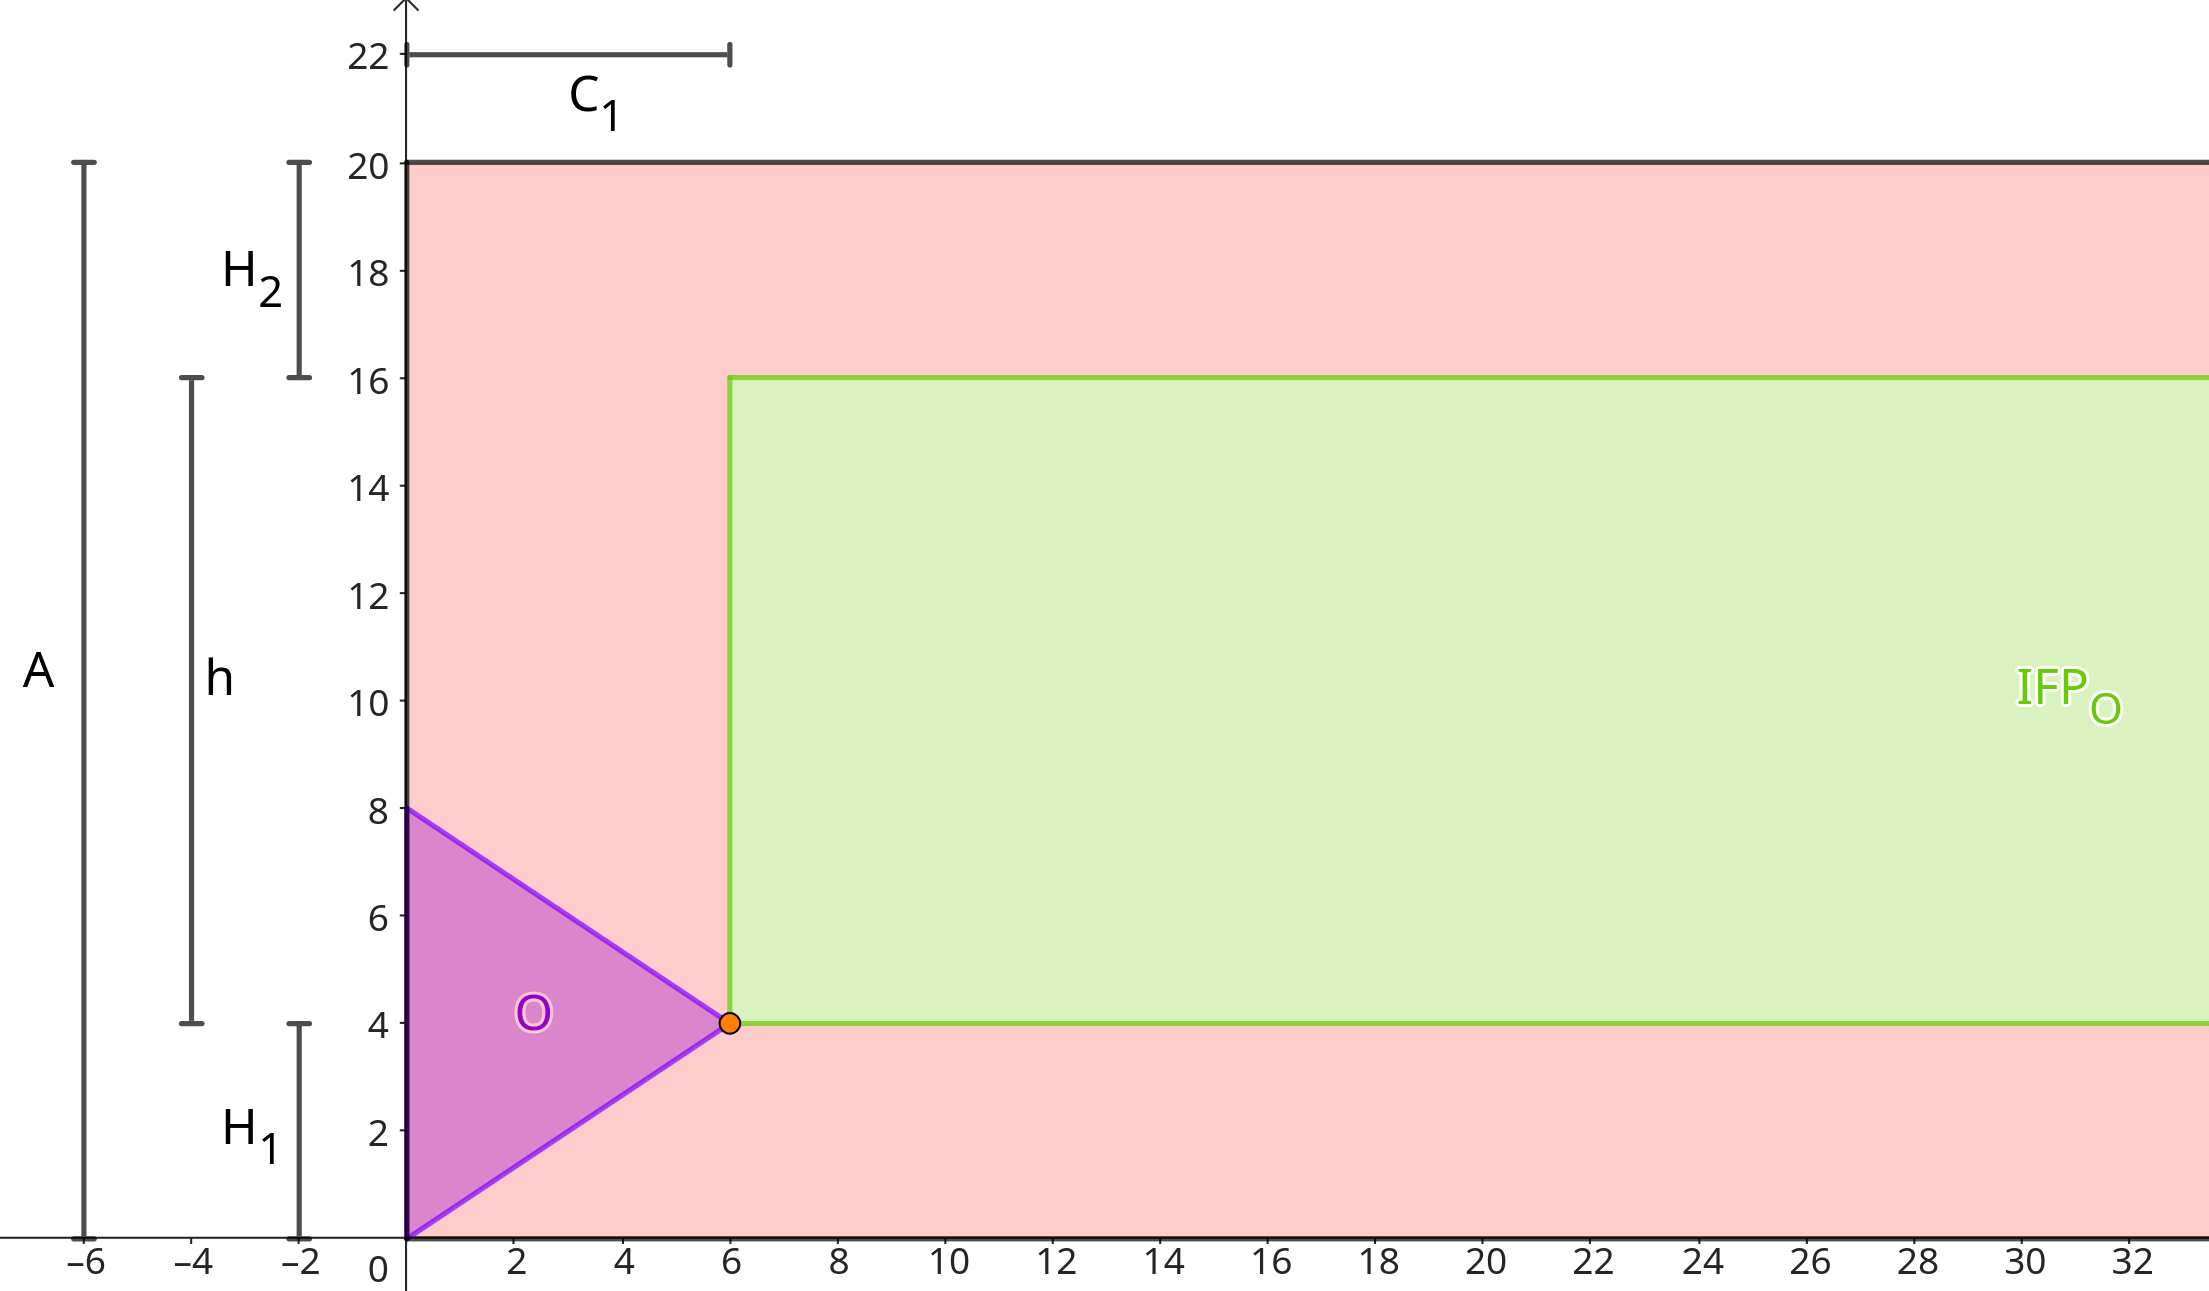
\includegraphics[width=.67\textwidth]{imagens_bl/IFPo.png}
    \caption{A área em verde é o IFP do polígono $O$.}
    \label{fig:f2}
\end{figure}

No exemplo da Figura~\ref{fig:f2}, o retângulo delimitado em preto é a faixa e queremos posicionar $O$ em seu interior. O $IFP_O$ está representado na figura pela área em verde e o ponto de referência $P$ é o em destaque laranja. Na figura, $H_1$ e $H_2$ representam, respectivamente, as distâncias entre $P$ e o ponto mais baixo de $O$ e entre $P$ e o ponto mais alto de $O$, e $h$ é a distância vertical restante para posicionar $P$. Além disso, $P$ só pode ser colocado horizontalmente à direita de $C_1$, distância entre $P$ e o ponto mais à esquerda de $O$. No desenho, $O$ estaria alocado no ponto mais à esquerda e abaixo possível.

Agora que analisamos a relação de $O$ com o recipiente, considere que queremos entender a interação entre os polígonos $M$ e $O$ presentes na Figura~\ref{fig:f3a}, para garantir que um não irá sobrepor o outro. Uma forma de fazer isso é manter $M$ parado e, garantindo que $O$ encoste nele o tempo todo, transladar $O$ ao seu redor, trançando o caminho feito pelo ponto de referência de $O$. O polígono formado por esse caminho é o que chamamos de {\it No-Fit Polygon (NFP)} e seu interior indica onde haverá sobreposição entre os dois, se colocarmos o ponto de referência de $O$. Caso o ponto de referência esteja no exterior do NFP, $O$ e $M$ não se encostarão.

Ao longo desse trabalho, chamamos de $NFP_{MO}$ aquele em que $M$ está fixo e $O$ translada ao seu redor, como observado na Figura~\ref{fig:f3b}. É importante notar que seu desenho poderá ser diferente do $NFP_{OM}$, o NFP gerado se alterarmos qual polígono translada e qual está fixo.

\begin{figure} [h]
    \centering
    \begin{subfigure}{.42\textwidth}
        \centering
        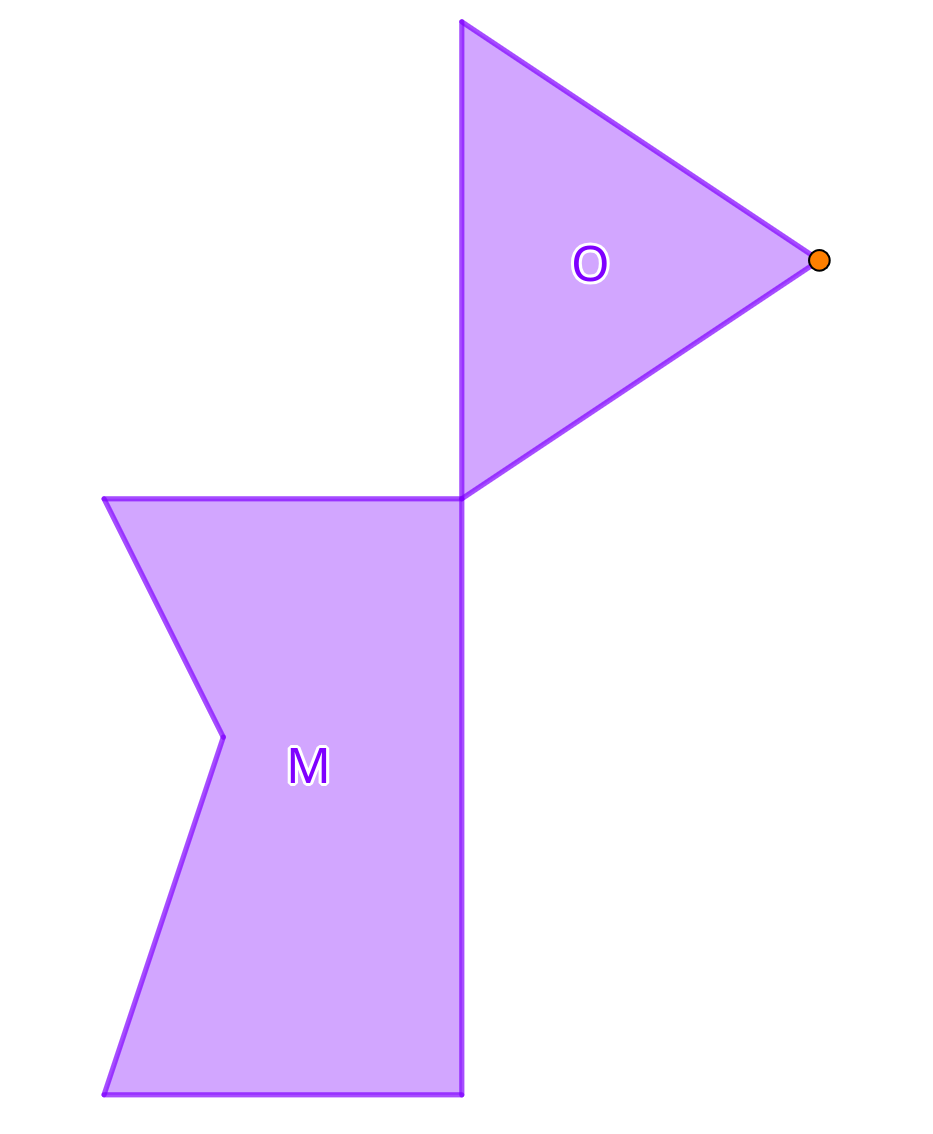
\includegraphics[width=\textwidth]{imagens_bl/O transl.png}
        \caption{$O$ transladando $M$.}
        \label{fig:f3a}
    \end{subfigure}
    \begin{subfigure}{.42\textwidth}
        \centering
        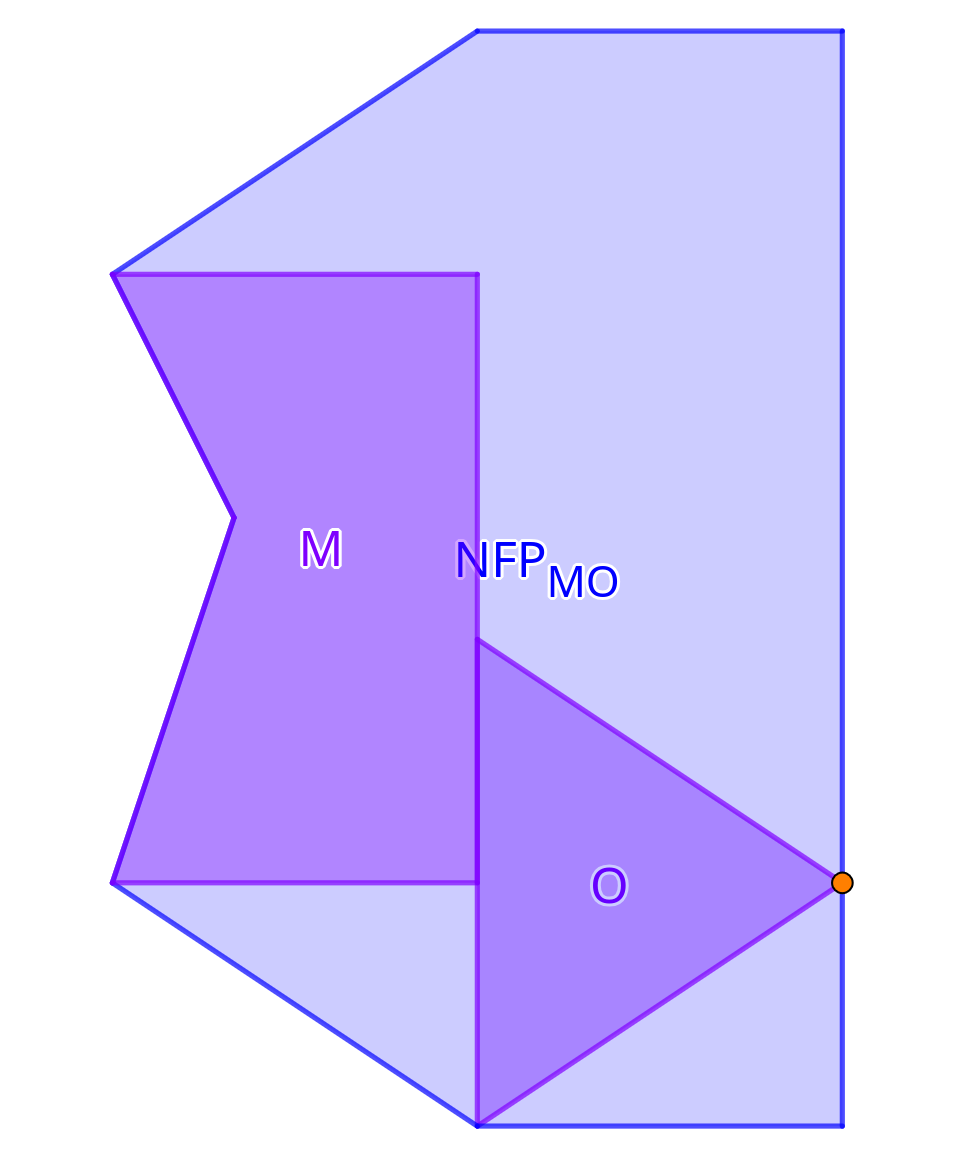
\includegraphics[width=\textwidth]{imagens_bl/M completo.png}
        \caption{$O$ transladando $M$ - $NFP_{MO}$.}
        \label{fig:f3b}
    \end{subfigure}
    \caption{O polígono $O$ sendo transladado ao redor de $M$ e o caminho feito pelo seu ponto de referência (em laranja) resultando no $NFP_{MO}$.}
    \label{fig:f3}
\end{figure}


Existem diversas maneiras de construir NFPs, como pode ser visto em \cite{irregular}. A mais intuitiva é a que acabamos de apresentar, transladando um em torno do outro, garantindo que estejam encostados e traçando a fronteira a partir do ponto de referência do polígono transladado. Vale destacar que, no nosso problema, a orientação dos polígonos é fixa, ou seja, eles não rotacionam.

Os algoritmos para calcular NFPs de polígonos convexos são mais simples, enquanto os para cálculo de não convexos são bem mais complicados. Portanto, quando um polígono (ou ambos) não é convexo, iremos decompô-lo em polígonos convexos menores (que chamamos de partes), para facilitar os cálculos, e o NFP será montado a partir da translação de cada parte separadamente. O NFP final de itens não convexos é constituído de partes que se sobrepõem e é importante citar que o item apenas estará em uma posição válida se ele não estiver no interior de nenhuma das partes.

\begin{figure}[H]
    \centering
    \begin{subfigure}{.24\textwidth}
        \centering
        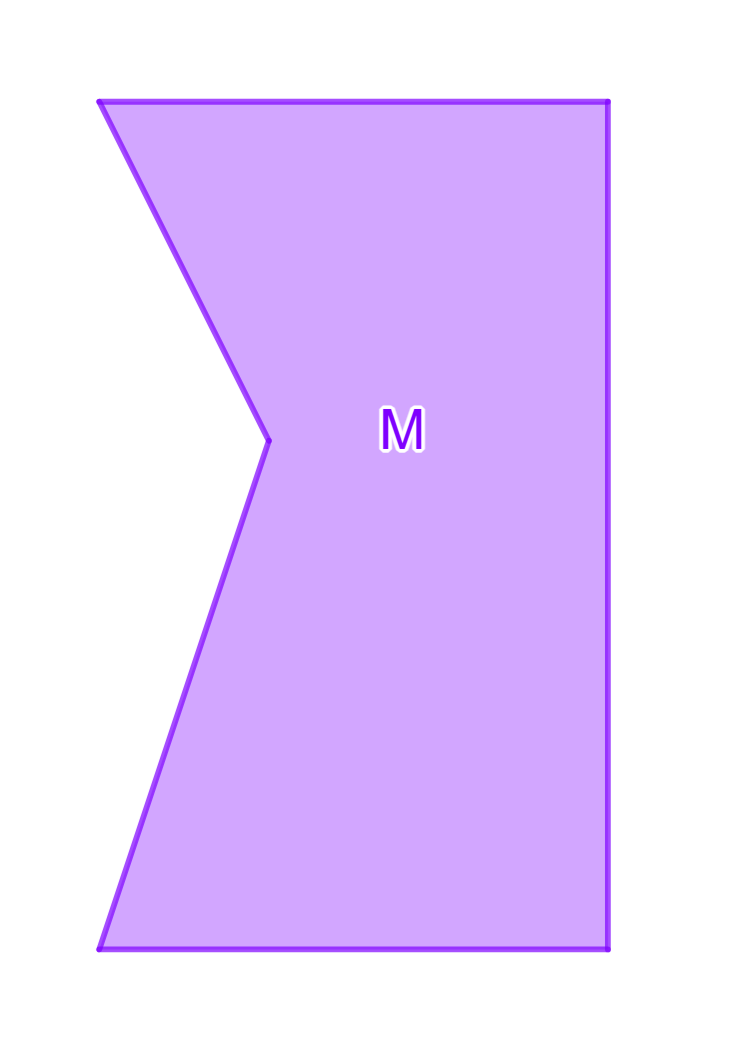
\includegraphics[width=\textwidth]{imagens_bl/M_solo.png}
        \caption{Polígono $M$ não convexo.}
        \label{fig:f4a}
    \end{subfigure}
    \hspace{1cm}
    \begin{subfigure}{.24\textwidth}
        \centering
        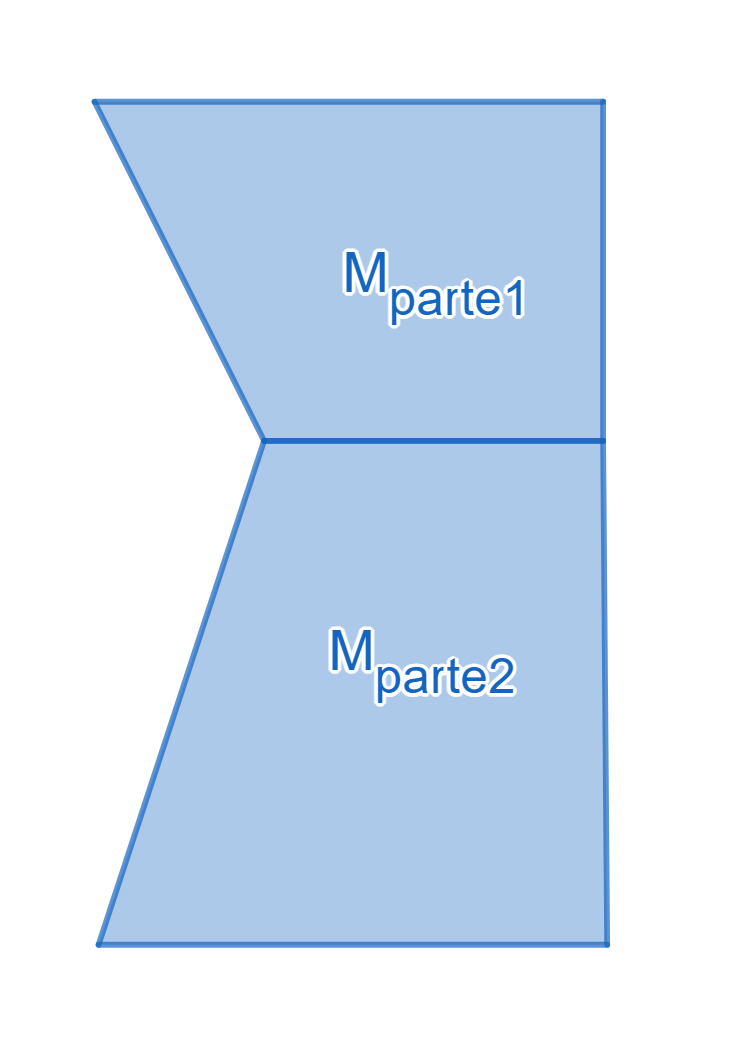
\includegraphics[width=\textwidth]{imagens_bl/M_12.png}
        \caption{Partes 1 e 2 convexas de $M$.}
        \label{fig:f4b}
    \end{subfigure}
    \caption{Polígono $M$ separado em duas partes por não ser convexo.}
    \label{fig:f4}
\end{figure}

Perceba que o polígono $M$ apresentado anteriormente não é convexo. Para construir o $NFP_{MO}$, podemos decompô-lo ele em dois polígonos convexos, como possível observar nas Figuras~\ref{fig:f4a} e~\ref{fig:f4b}, e vamos construir o NFP de $O$ com relação às partes 1 e 2 do polígono $M$. Nas Figuras~\ref{fig:f5a} e~\ref{fig:f5b} temos $O$ transladando cada parte de $M$. Observe que deve ser feito um ajuste final no posicionamento de cada parte do NFP ao juntá-las, tendo em mente qual a posição de uma parte em relação à outra. Na Figura~\ref{fig:f6a} temos a junção das partes e na Figura~\ref{fig:f6b} temos o $NFP_{MO}$ por essa montagem, cujo contorno exterior podemos observar ser exatamente o mesmo da Figura~\ref{fig:f3b}.

\begin{figure}[H]
    \centering
    \begin{subfigure}{.48\textwidth}
        \centering
        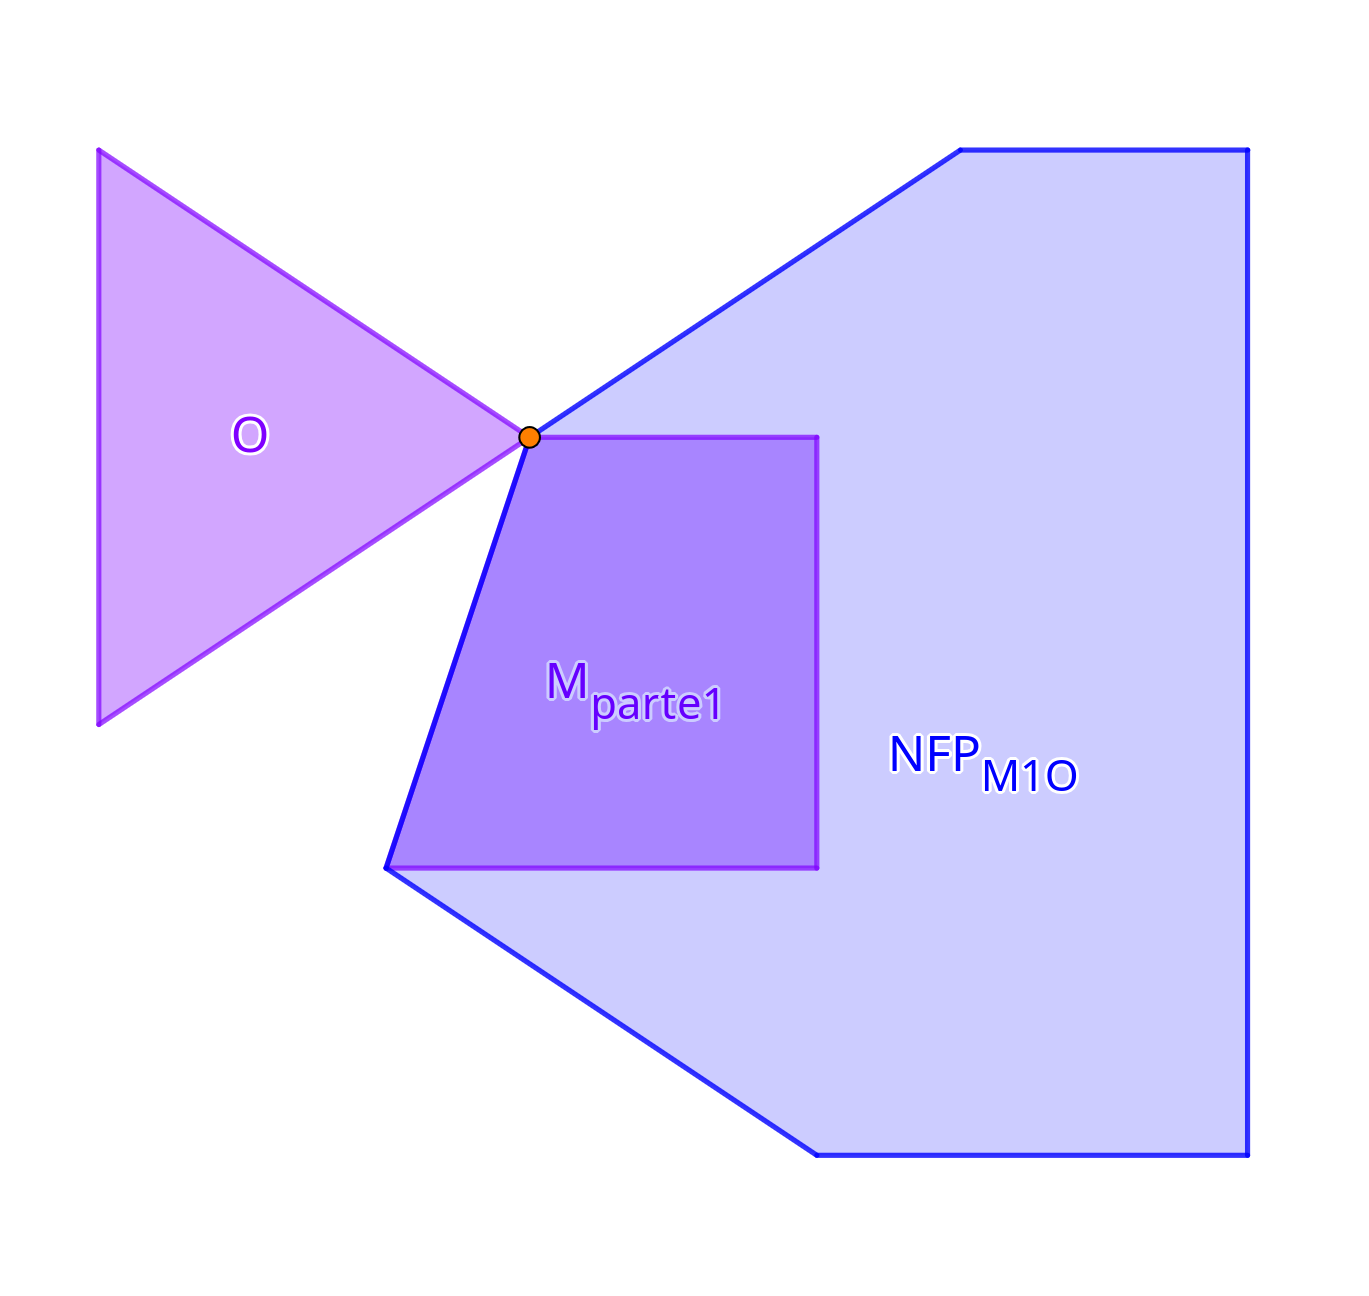
\includegraphics[width=\textwidth]{imagens_bl/NFPm1o.png}
        \caption{$O$ transladando $M_{parte1}$ - $NFP_{M_1O}$.}
        \label{fig:f5a}
    \end{subfigure}
    \hfill
    \begin{subfigure}{.48\textwidth}
        \centering
        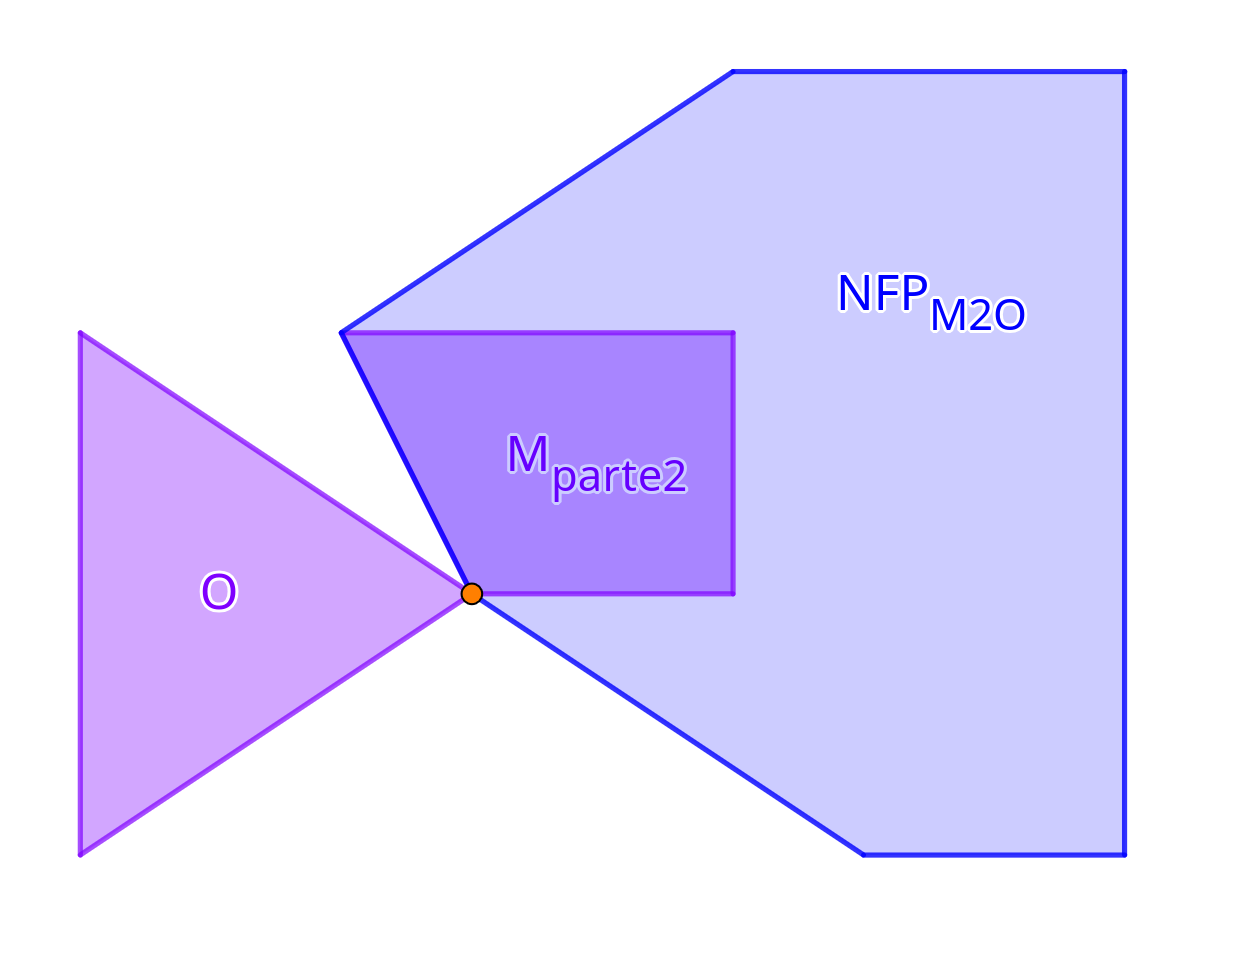
\includegraphics[width=\textwidth]{imagens_bl/NFPm2o.png}
        \caption{$O$ transladando $M_{parte2}$ - $NFP_{M_2O}$.}
        \label{fig:f5b}
    \end{subfigure} 
    \caption{Montagem das duas partes do $NFP_{MO}$.}
    \label{fig:f5}  
\end{figure}



\begin{figure}[H]
    \centering
    \begin{subfigure}{.49\textwidth}
        \centering
        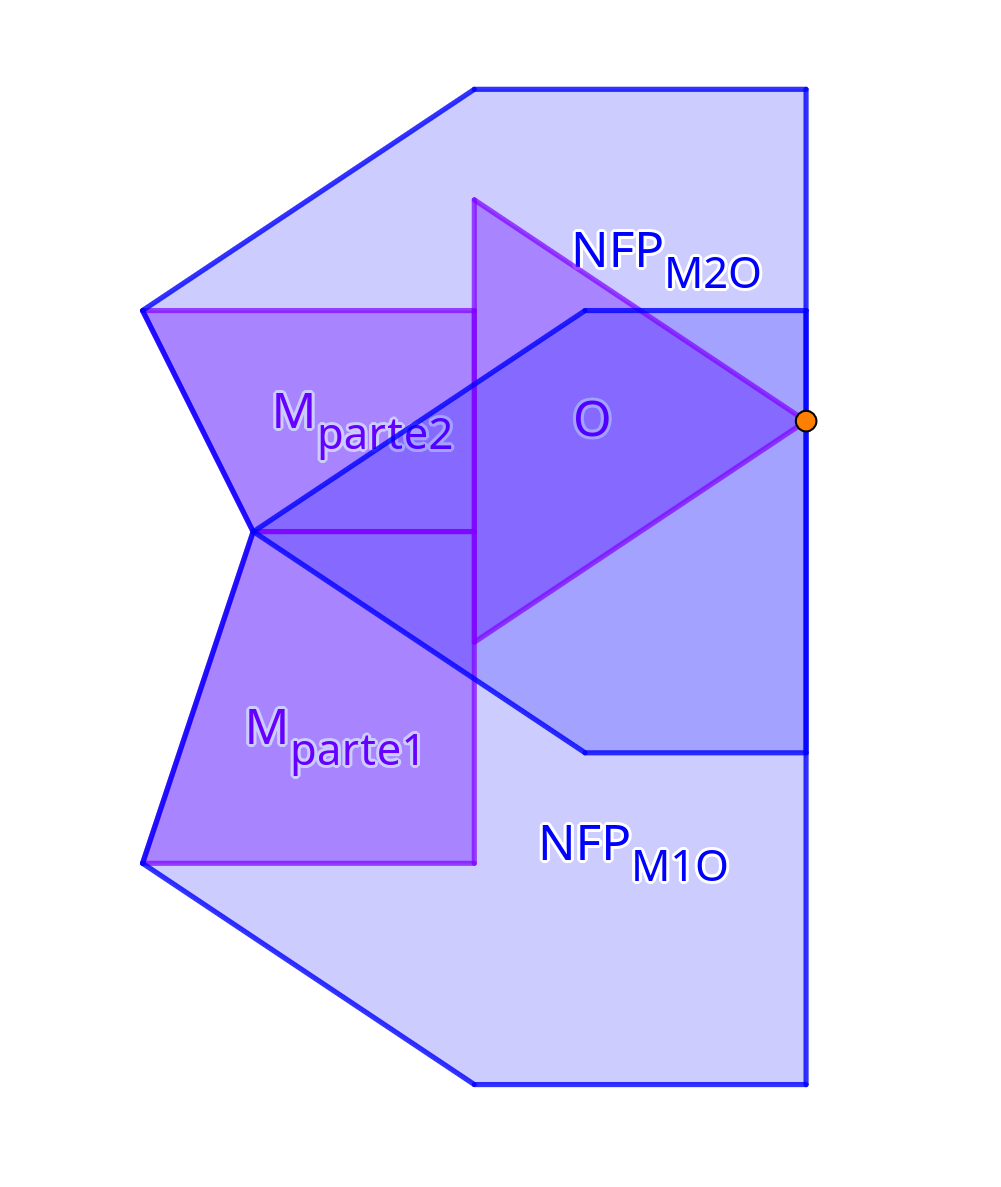
\includegraphics[width=.93\textwidth]{imagens_bl/NFPmo e M.png}
        \caption{Partes de $M$, $O$ e as partes de $NFP_{MO}$.}
        \label{fig:f6a}
    \end{subfigure}
    \hfill
    \begin{subfigure}{.41\textwidth}
        \centering
        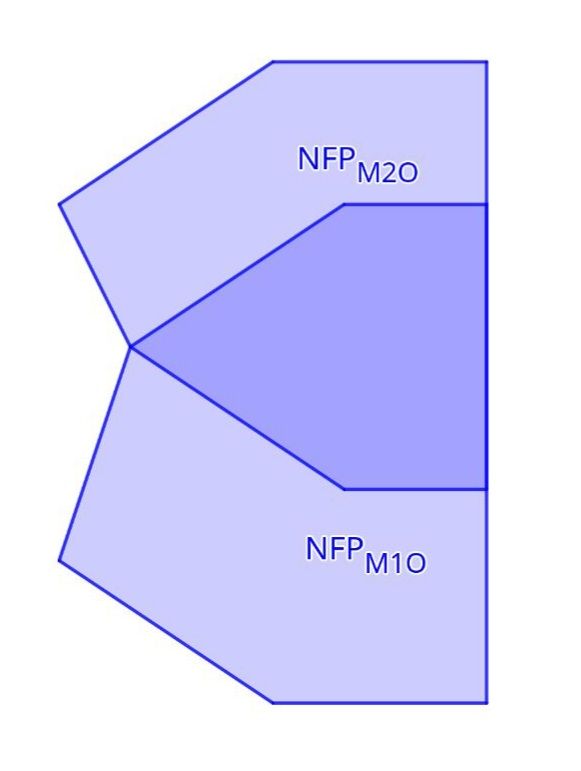
\includegraphics[width=\textwidth]{imagens_bl/NFPmo_partes.jpg}
        \caption{NFP a partir das duas partes.}
        \label{fig:f6b}
    \end{subfigure}
    \caption{Junção das duas partes do $NFP_{MO}$.}
    \label{fig:f6}
\end{figure}

Na próxima seção vamos colocar todas as ferramentas apresentadas em uso para implementar uma heurística que resolva o problema de cortar itens irregulares como esses, convexos e não convexos, em faixa.

\section{Heurística construtiva para resolver o problema de corte de itens irregulares} \label{sec:BL}

Uma heurística é uma forma de encontrar uma solução suficientemente boa para um problema de otimização, diminuindo os gastos computacionais e de tempo que seriam gastos para encontrar uma solução ótima. Dada uma lista de polígonos ordenados segundo algum critério, a heurística {\it Bottom-Left}, estudada por meio de \cite{irregular}, consiste em alocar um polígono de cada vez no ponto mais à esquerda possível da faixa e, caso haja mais de um ponto, mais abaixo. Dessa forma, é uma heurística simples para problemas de empacotamento, que iremos aplicar para resolver o problema citado na Seção \ref{sec:irregular}.

Utilizando como exemplo a Figura~\ref{fig:f7}, temos os polígonos já conhecidos $M$ e $O$ e um quadrado $N$ de lado 6, na faixa de altura $A = 20$. A ordem de posicionamento escolhida é alfabética e, dado que $M$ e $N$ já estão situados de acordo com a Figura~\ref{fig:f7} e o IFP de $O$ é o mesmo da Figura~\ref{fig:f2}, vamos alocar $O$ utilizando o $NFP_{MO}$, o $NFP_{NO}$ e o $IFP_O$.

\begin{figure}[H]
    \centering
    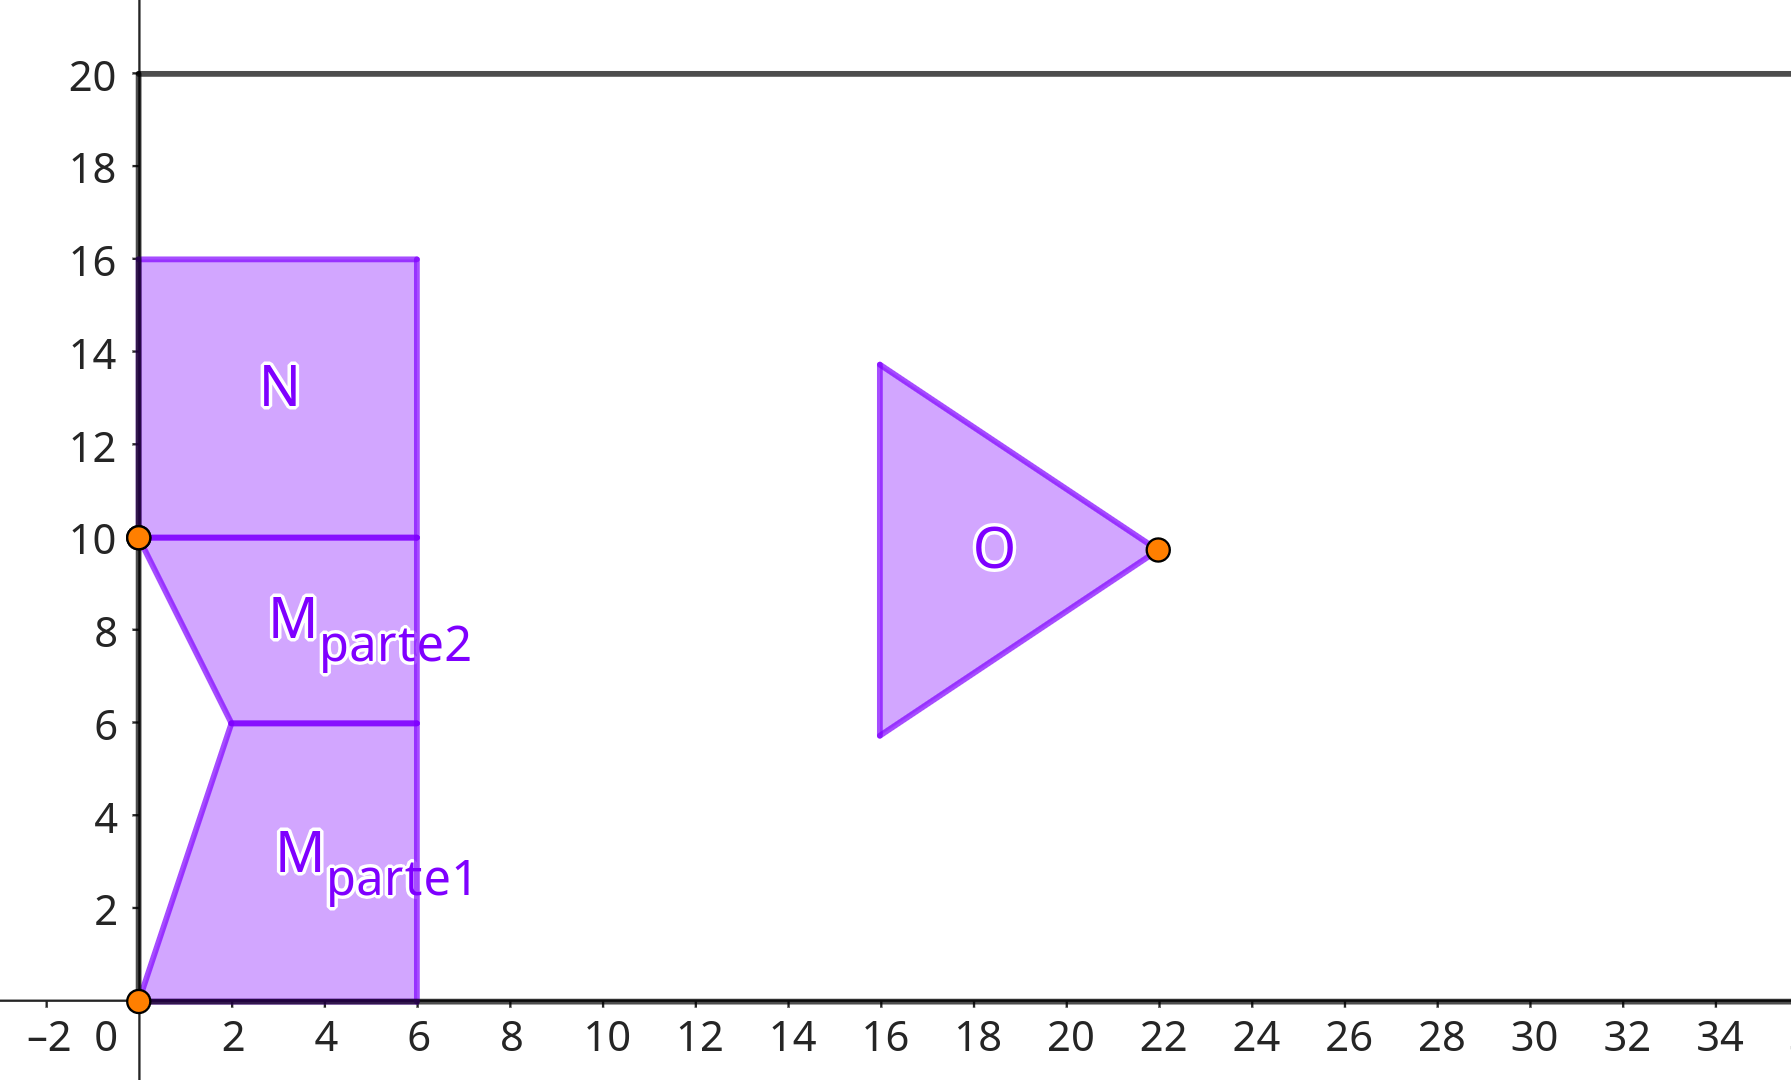
\includegraphics[width=.7\textwidth]{imagens_bl/Posicao.png}
    \caption{Polígonos $M$ e $N$ alocados na faixa e $O$ aguardando alocação.}
    \label{fig:f7}
\end{figure}


Uma maneira de encontrar as possíveis posições para alocar o polígono $O$ é calcular todas interseções das arestas entre $NFP_{MO}$, $NFP_{NO}$ e $IFP_O$ e remover as que não forem viáveis. Note que isso é prático pois, ao alocarmos um item, sempre é possível encaixá-lo melhor ao garantir que ele esteja encostado ao menos em duas arestas (sejam elas de itens ou da fronteira do recipiente).

Observe na Figura~\ref{fig:f8} os NFPs deslocados baseados na alocação do seu respectivo polígono base e na Figura~\ref{fig:f9} todas as intersecções. Os pontos em vermelho são aqueles que estão na área proibida de alguma das restrições, ou seja, dentro de algum NFP ou no exterior do IFP. Ademais, podemos ver que entre os cinco pontos permitidos, que estão em verde, não existe um mais à esquerda (dado que todos tem mesma abscissa) e o mais abaixo é aquele onde $O$ deve ser posicionado (ponto $P_5$).

Na Figura~\ref{fig:f10} temos então o polígono $O$ em sua posição final de acordo com a heurística \textit{Bottom-Left}, em $P_5$.

\begin{figure} [H]
    \centering
    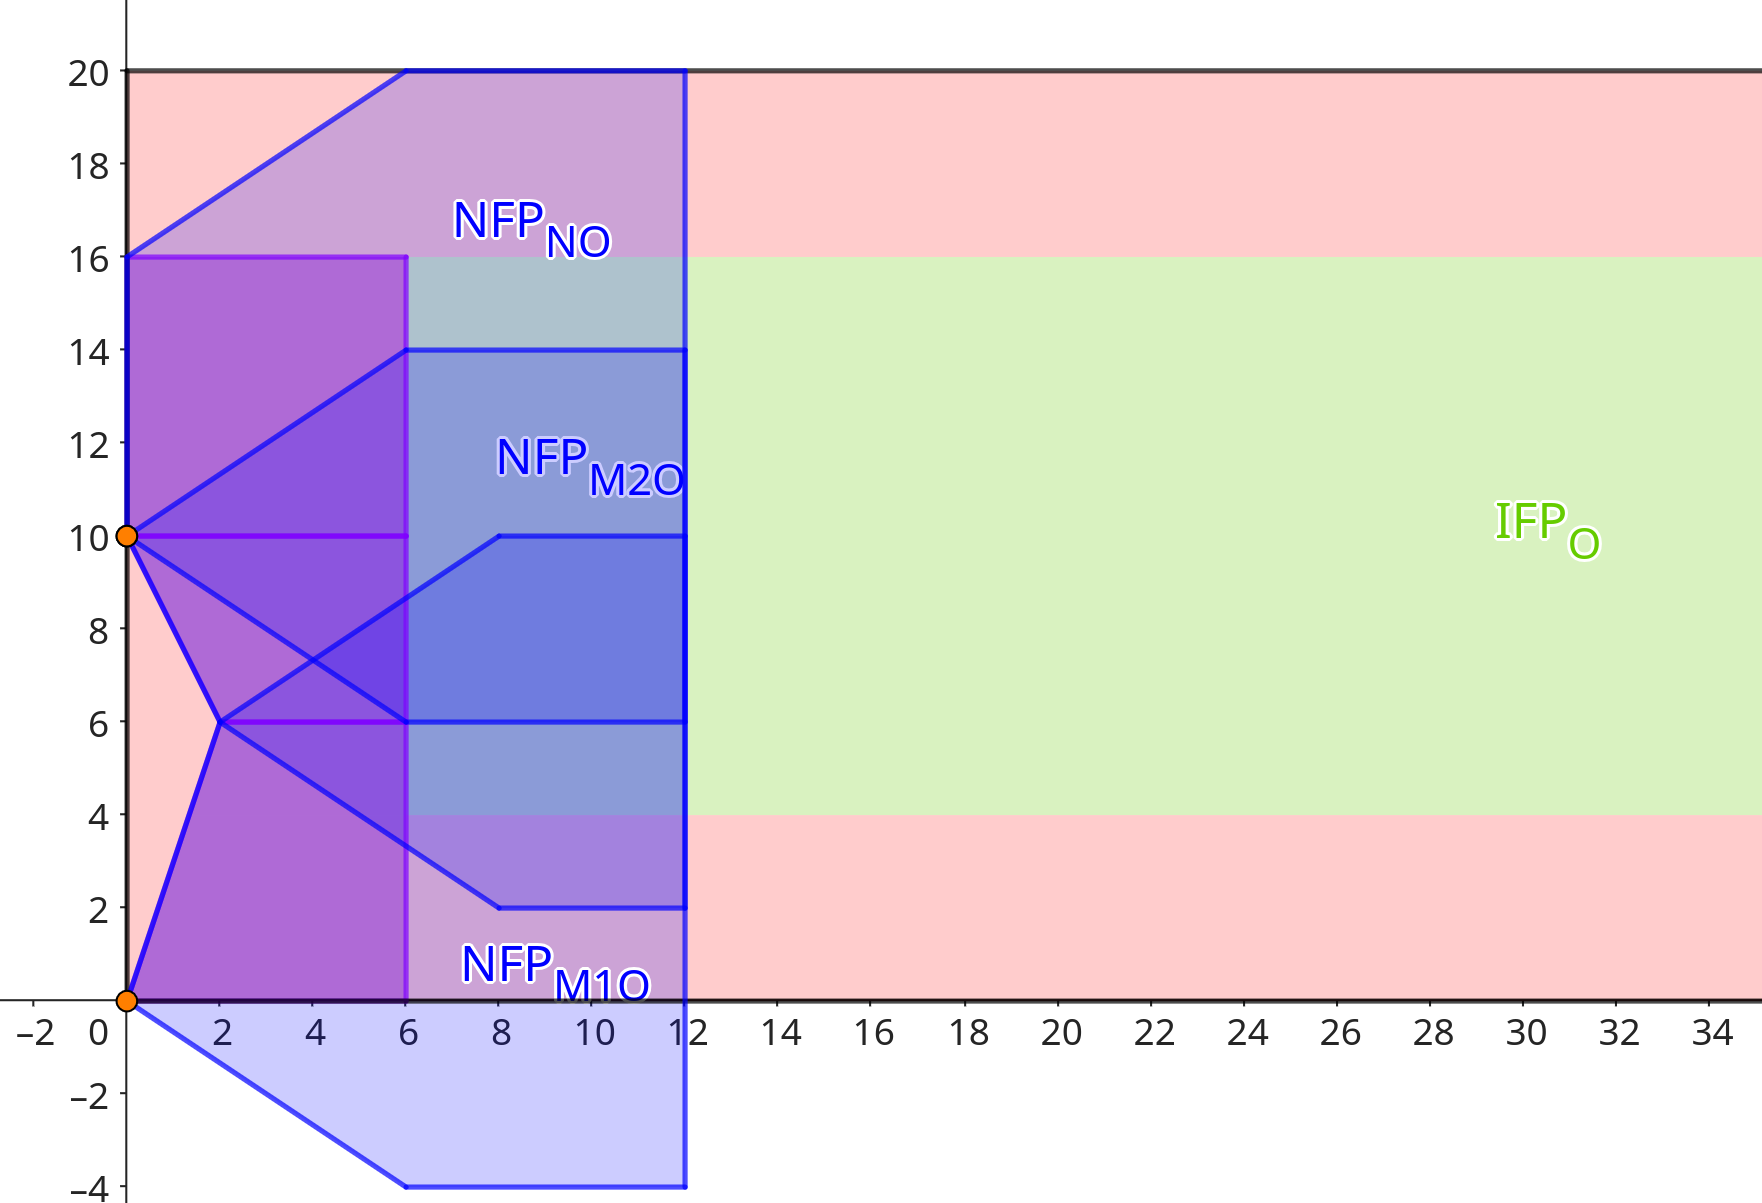
\includegraphics[width=.75\textwidth]{imagens_bl/Polig e NFP.png}
    \caption{Polígonos $M$ e $N$, com os respectivos NFPs em relação a $O$ (note que os NFPs estão posicionados para encaixar perfeitamente com o polígono fixo referente a ele). As intersecções gerarão os possíveis pontos para alocar o ponto de referência de $O$.}
    \label{fig:f8}
\end{figure}

\begin{figure} [H]
    \centering
    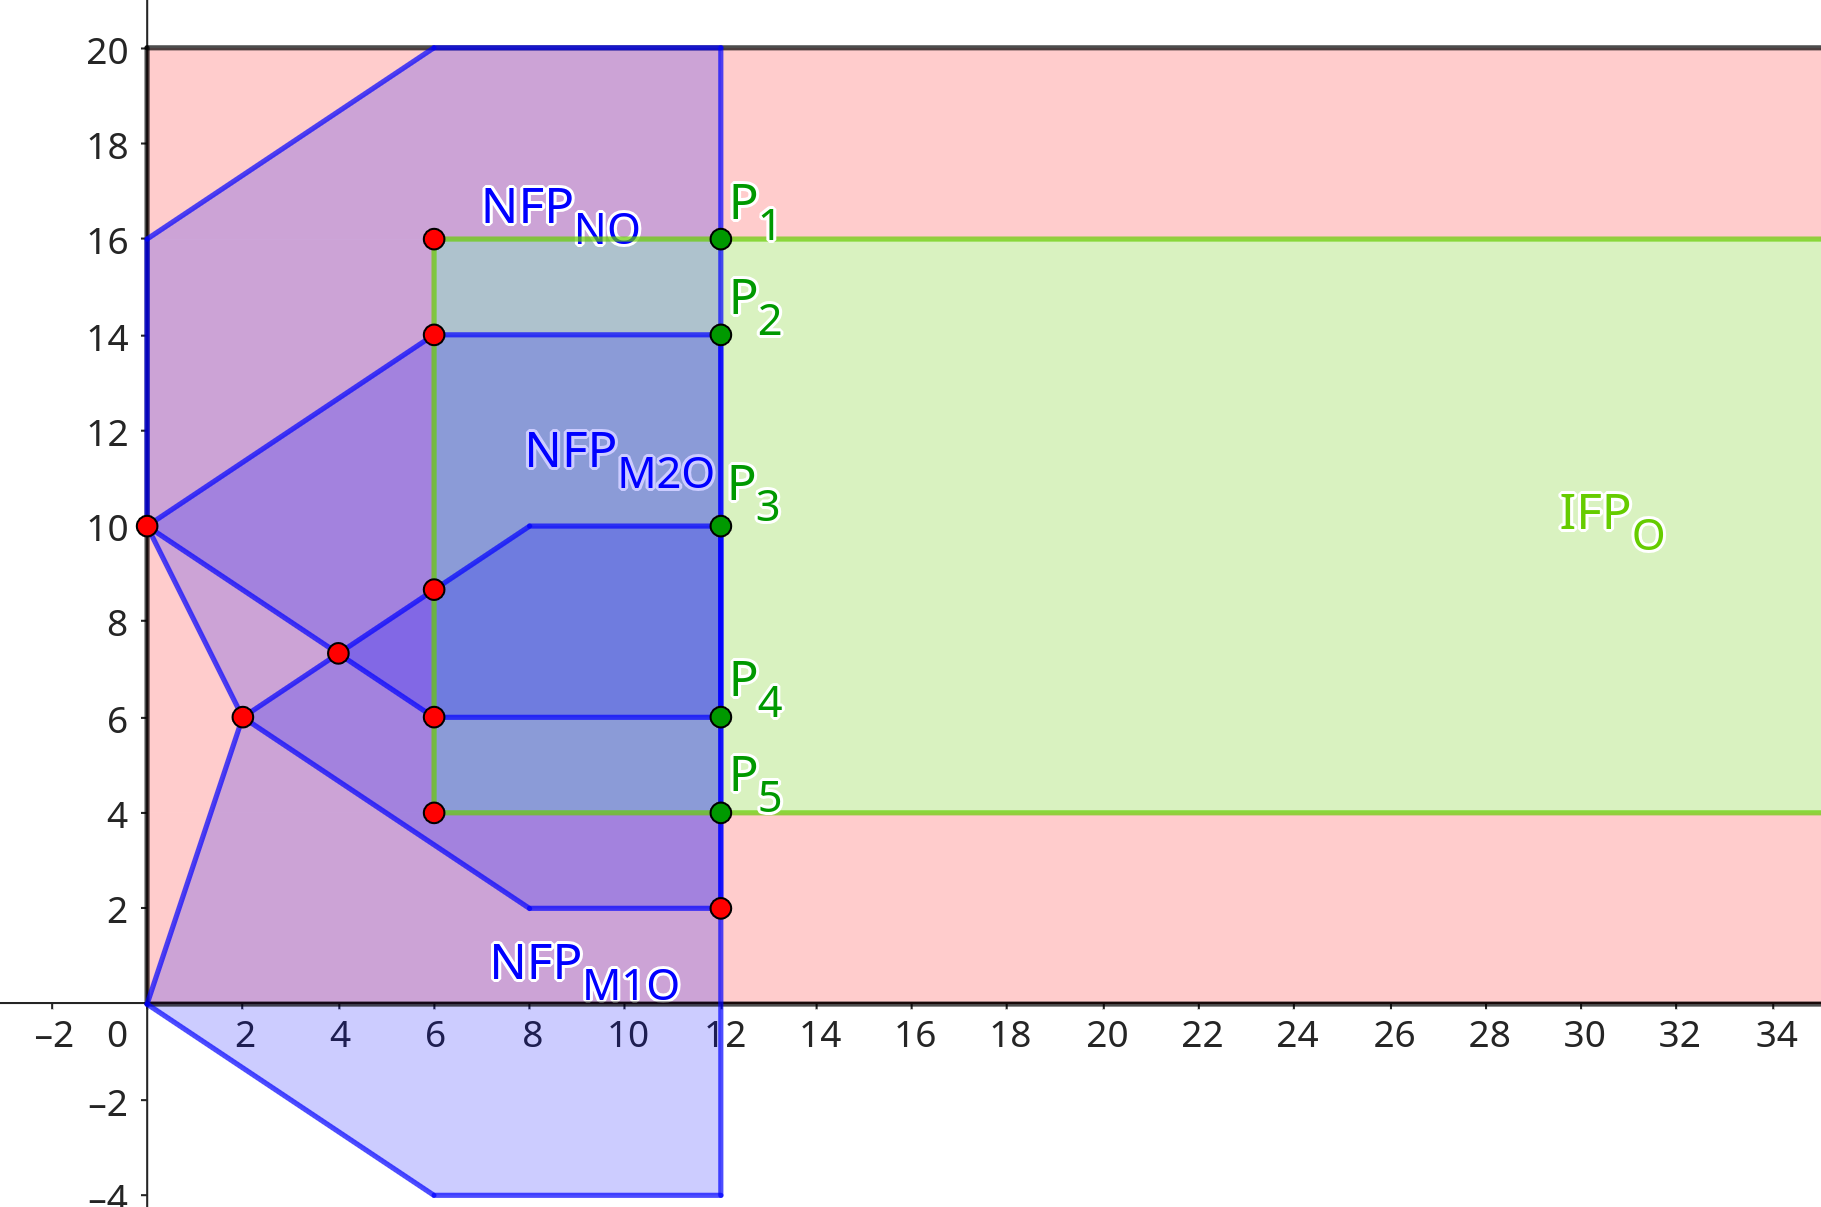
\includegraphics[width=.75\textwidth]{imagens_bl/NFP e pontos.png}
    \caption{$NFP_{M_1O}$, $NFP_{M_2O}$, $NFP_{NO}$ e os pontos de intersecção entre todos e o $IFP_O$, onde os pontos em vermelho são posições proibidas e os em verde são posições viáveis.}
    \label{fig:f9}
\end{figure}


\begin{figure} [H]
    \centering
    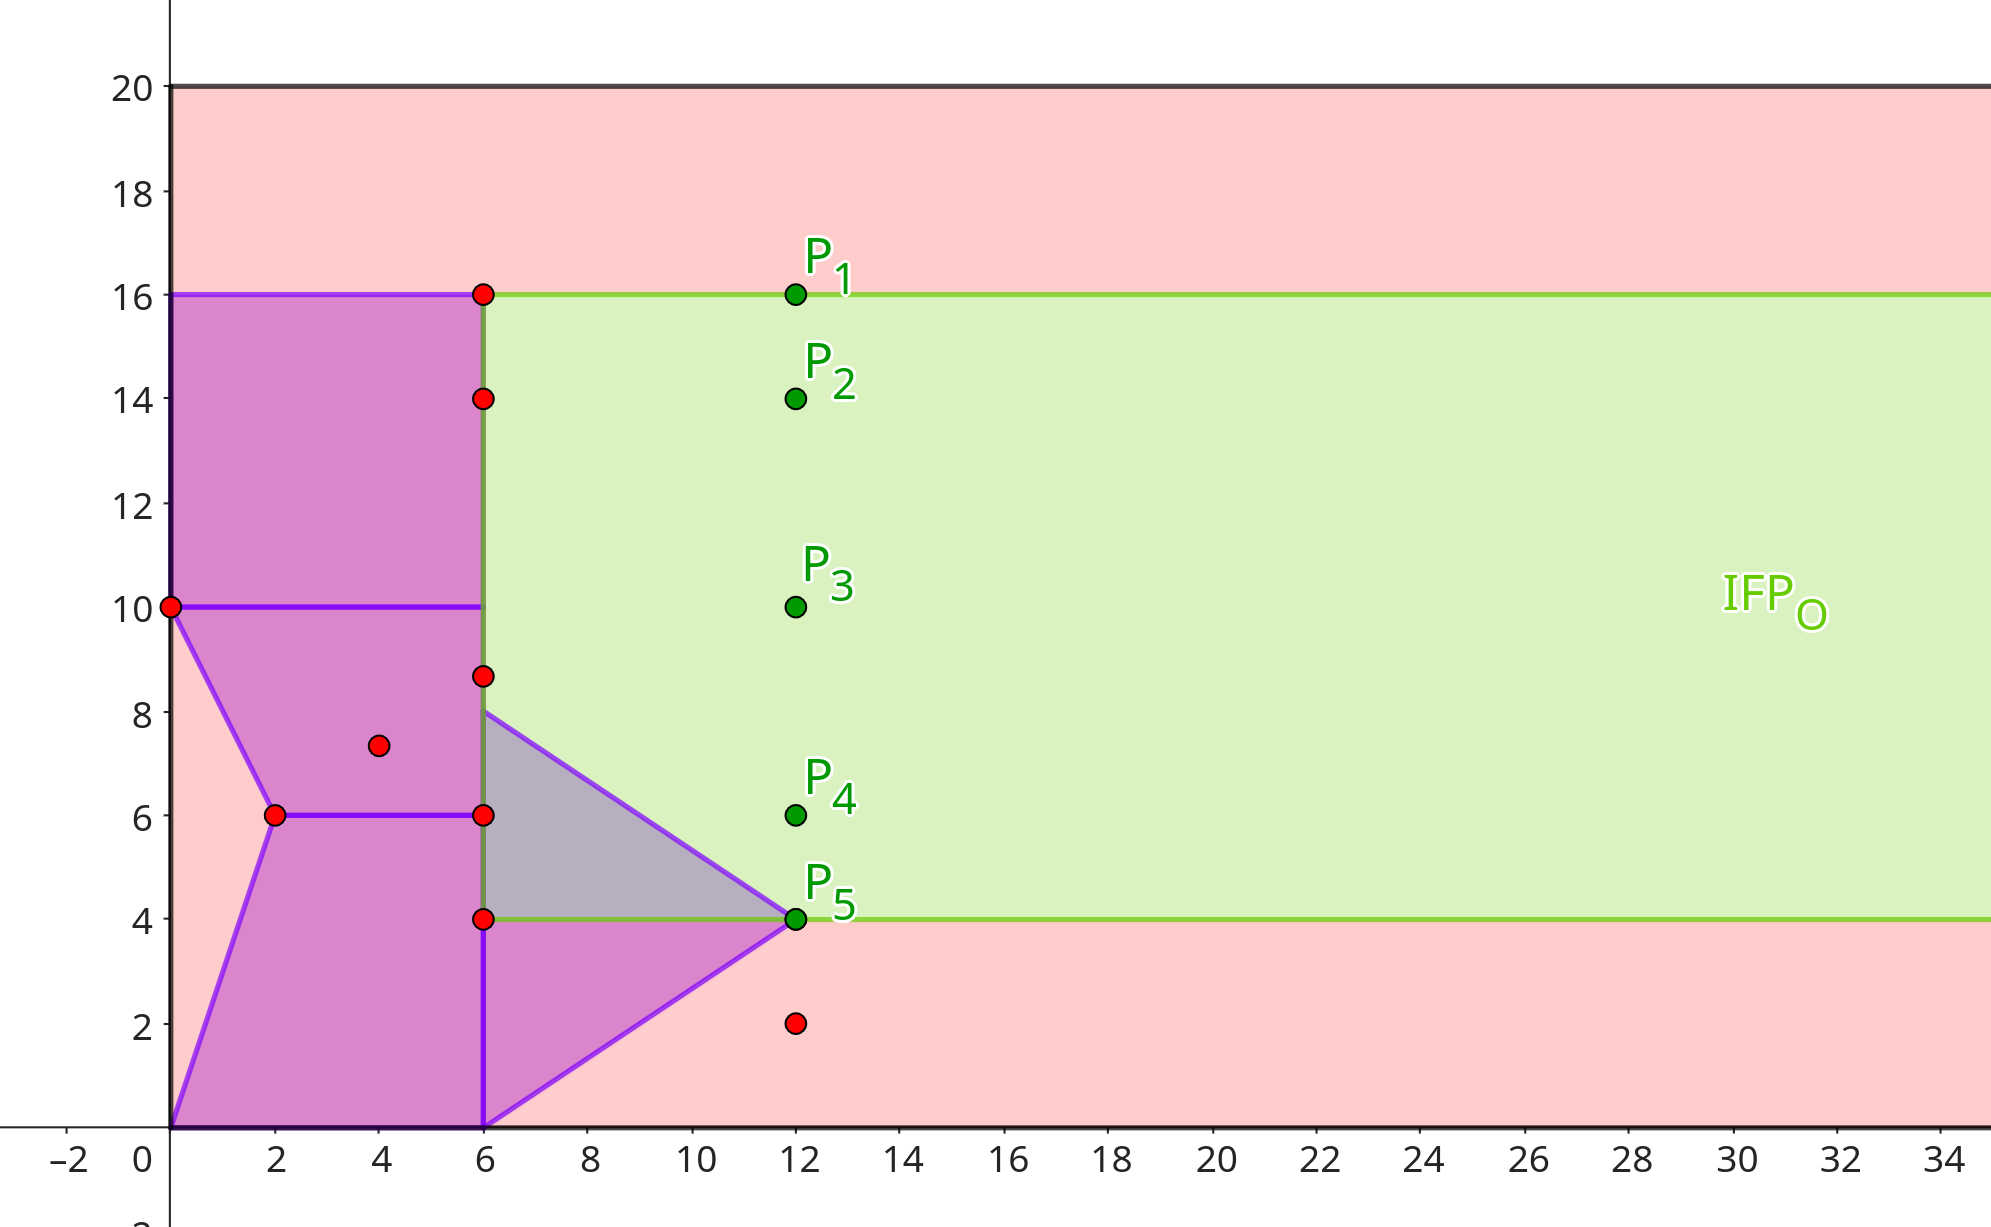
\includegraphics[width=.75\linewidth]{imagens_bl/pontosfin.png}
    \caption{Todos os pontos de intersecção de $O$ e a posição final onde foi alocado ($P_5$).}
    \label{fig:f10}
\end{figure}


Agora que temos todas as ferramentas de alocação bem sedimentadas, vamos para a resolução em si. Para resolver o problema de corte de itens irregulares em faixa foi implementado um código em linguagem C com a heurística {\it Bottom-Left}. O programa lê em um arquivo ``general\_data.txt'' a altura $A$ da faixa, o número $m$ de itens e $m$ linhas seguintes contendo o número de cópias de cada item. Em seguida, é lida uma lista de $m$ arquivos ``pieceX.txt'' que diz o número de partes do item $X$, representado por um número de 1 a $m$, e lista os vértices em sentido anti-horário para cada parte, considerando que o primeiro ponto da primeira parte é $(0,0)$, que é o ponto de referência de $X$.

Por último, o programa lê $m^2$ arquivos ``NFP\_i\_0\_j\_0.txt'' com as partes e vértices de cada NFP, construídos pensando no ponto de referência do item $i$ em $(0,0)$ e o item $j$ transladando ao seu redor, ambos com rotação de $0$ graus.

A estrutura de dados consiste em armazenar em uma estrutura referente a um item $X$ seu polígono, seus pontos extremos, o número de cópias, a lista de $NFP_{XJ}$ (onde $J = 1, \dots, m$), o vértice do ponto de referência em sua alocação final para cada cópia e uma variável auxiliar para numerar quantas cópias já foram alocadas.

Ainda no terminal, antes de executar o programa, é usado um {\it makefile} para compilar o programa e gerar um executável, especificando nele quais as instâncias a serem resolvidas e qual ordenação será utilizada para a {\it Bottom-Left}. As ordenações foram separadas em duas categorias que são combinadas na hora de aplicar: método e sentido da ordenação. O método é dado por um número de 1 a 6 que dita qual valor a ser observado para ordenar o itens, as opções são as seguintes:

\begin{enumerate}
    \item ordenação baseada na área do item;
    \item ordenação baseada na área do menor retângulo que contém o item;
    \item ordenação baseada no comprimento de cada item (diferença entre pontos extremos em relação ao eixo $X$);
    \item ordenação baseada na altura de cada item (diferença entre pontos extremos em relação ao eixo $Y$);
    \item ordenação baseada na divisão da área do item pela área do menor retângulo que o contém;
    \item ordenação baseada na divisão entre o comprimento (diferença entre pontos extremos em relação ao eixo $X$) e altura (diferença entre pontos extremos em relação ao eixo $Y$) de cada item.
\end{enumerate}

Em relação ao sentido da ordenação temos apenas dois valores possíveis: $1$ ordena o índice com valores dos cálculos do método de forma decrescente e $2$ de forma crescente. Então, após a leitura de dados, o programa passa pelas seguintes etapas:
\begin{enumerate}
    \item Ordena todos os itens (incluindo as cópias) utilizando a opção escolhida;
    \item Para cada item $a$, a partir da ordem do Passo 1:
    \begin{enumerate}
        \item Calcula o $IFP_a$;
        \item Verifica se o vértice inferior esquerdo do $IFP_a$ é válido (ou seja, se não está no interior de nenhum $NFP_{ai}$, com $i$ os itens já alocados na faixa);
        \item Em caso positivo, define $M$ (que guarda o melhor ponto para alocar um item $a$ a cada iteração) como esse e pula para o Passo 2.(e);
        \item Caso contrário:
        \begin{enumerate}
            \item Defina $M$ como um ponto de coordenadas $(g,0)$, em que $g$ é um valor muito grande que não pretendemos alcançar no comprimento da faixa (calculado, por exemplo, somando o comprimento de todos os itens a serem alocados);
            \item Calcula todas as intersecções duas a duas entre os $NFP_{ai}$ e $NFP_{aj}$, com $i$ e $j$ os itens já alocados na faixa;
            \item Calcula todas as intersecções entre os $NFP_{ai}$, com $i$ os itens já alocados na faixa, com o $IFP_a$;
            \item Para cada intersecção $I$ encontrada, se a coordenada $x$ de $I$ é menor do que a coordenada $x$ de $M$ (ou se a coordenada $x$ de $I$ é igual à coordenada $x$ de $M$ e a coordenada $y$ de $I$ é menor do que a coordenada $y$ de $M$), atualiza $M$ com o valor de $I$;
        \end{enumerate}
        \item Aloca o item $a$ no ponto $M$ da faixa.
    \end{enumerate}
\end{enumerate}

%Conforme cada ponto é calculado, sua validade só será averiguada se for mais à esquerda (ou tão à esquerda quanto e mais abaixo) que o último ponto dado como válido.

Por fim o programa imprime um arquivo em Latex utilizando a ferramenta {\it Tikz} do leiaute correspondente, em que o recipiente é representado em azul, o comprimento obtido é a linha vertical pontilhada e os itens são coloridos (itens não convexos são representados por suas partes convexas conectadas, de mesma cor). Imprime também as informações de comprimento mínimo alcançado e tempo de execução num único arquivo de texto para facilitar sua disposição em forma de tabela (como a da Seção \ref{sec:experimentosbl}).


\subsection{Experimentos numéricos} \label{sec:experimentosbl}


Para que fosse feito o teste do código, implementado em linguagem C, executamos a heurística {\it Bottom-Left} com todas as combinações de método e sentido de ordenação apresentadas na Seção~\ref{sec:BL}, totalizando doze variantes da heurística, chamadas de $BL_{MS}$, em que $M$ representa o método e $S$ o sentido da ordenação. As variações foram aplicadas em vinte e nove instâncias clássicas da literatura\footnote{\url{https://www.euro-online.org/websites/esicup/data-sets}, acessado em 20/02/2025.}, as presentes nas tabelas~\ref{tab:t1} e~\ref{tab:t2}.

Os experimentos foram executados em um computador de 8GB de memória, processador Intel® Core™ i5-8250U x 8 e Sistema Operacional Ubuntu 24.04.2 LTS. Tanto o código em C quanto os arquivos base das instâncias e todos os leiautes obtidos ao longo deste trabalho de Iniciação Científica podem ser acessados em \url{https://sites.icmc.usp.br/andretta/pinheiro-2025/}.


Os resultados obtidos foram divididos em duas tabelas~\ref{tab:t1} e~\ref{tab:t2}. A coluna ``Instância'' contém o nome de cada instância utilizada, a ``Itens'' retrata o número de itens da instância (incluindo as cópias de cada item). Em seguida, cada grupo de duas colunas representa o resultado da execução de uma combinação $BL_{MS}$, em que $M = \{1, 2, \dots, 6\}$ e $S = \{1, 2\}$. A coluna ``Comp'' representa o comprimento obtido para a instância pela heurística $BL_{MS}$ correspondente e a coluna ``T(s)'' apresenta o tempo em segundos que a heurística levou para resolver cada instância. O valor em destaque em cada linha é o menor valor entre todos os resultados para aquela instância. Na Tabela~\ref{tab:t1}, temos as 6 variações da heurística que apresentaram as maiores quantidades de instâncias para as quais se obteve melhores comprimentos, ordenadas da que obteve maior quantidade de melhores resultados para a que obteve menor quantidade. Na Tabela~\ref{tab:t2} estão as variantes restantes da heurística.

Como podemos observar na Tabela~\ref{tab:t1}, a ordenação dos itens de forma decrescente baseada no comprimento de cada um ($BL_{31}$) obteve o maior número de bons resultados (12 de 29 instâncias) e, assim como todas as variações, num tempo de execução muito pequeno para todas as instâncias. Para entender a disparidade existente entre as variações da heurística aplicadas a uma mesma instância, dividimos o menor valor de comprimento obtido para cada uma pelo maior. Assim, observamos a maior diferença de valores na instância {\it poly5A}, com razão $0,895$, e a menor na instância {\it poly1A}, com razão $0,715$. Ou seja, notamos que como nenhuma proporção resultou em $1$, variar a ordenação para aplicar a heurística gera resultados diferentes em todos os casos. Quando comparamos somente os resultados das heurísticas $BL_{31}$, $BL_{21}$, $BL_{52}$ e $BL_{11}$, as quatro com melhores resultados, a posição entre qual tem maior número de melhores resultados não foi alterada.





\begin{adjustwidth}{-2cm}{-2.5 cm}\centering\begin{threeparttable}[!htb]\centering
\renewcommand{\arraystretch}{1.2}%
    \caption{Resultados obtidos pelas 6 variações da heurística {\it Bottom-Left} que obtiveram maior quantidade de menores valores de solução.}
    \scriptsize{
        \begin{tabular}{|l|c|rr|rr|rr|rr|rr|rr|}\hline
        \multicolumn{1}{|c|}{} & \multicolumn{1}{c|}{} &  \multicolumn{2}{c|}{$BL_{31}$} & \multicolumn{2}{c|}{$BL_{21}$} & \multicolumn{2}{c|}{$BL_{52}$} &
        \multicolumn{2}{c|}{$BL_{11}$} &
        \multicolumn{2}{c|}{$BL_{12}$} &
        \multicolumn{2}{c|}{$BL_{22}$}\\
            Instância &Itens &Comp &T (s) &Comp &T (s) &Comp &T (s) &Comp &T (s) &Comp &T (s) &Comp &T (s) \\\hline
            albano &24  &\lgray11376,46 &0,42  &11818,58 &0,29  &13525,12 &0,36  &11818,58 &0,37  &14679,58 &0,42  &13959,22 &0,43 \\
            blaze1 &28  &\lgray28,67 &0,22  &31,20 &0,20  &34,34 &0,21  &30,35 &0,28  &32,14 &0,25  &36,67 &0,33 \\
            blaze2 &16  &\lgray21,50 &0,08  &22,10 &0,06  &25,29 &0,04  &\lgray21,50 &0,09  &22,50 &0,05  &24,93 &0,08 \\
            dagli &30  &75,47 &0,57  &73,33 &0,39  &89,92 &0,23  &\lgray67,69 &0,43  &86,35 &0,18  &78,40 &0,19 \\
            dighe1 &16  &\lgray146,96 &0,00  &167,06 &0,00  &165,75 &0,00  &163,26 &0,00  &203,00 &0,01  &187,03 &0,01 \\
            dighe2 &10  &\lgray145,56 &0,00  &163,23 &0,00  &165,16 &0,00  &154,30 &0,00  &182,78 &0,00  &166,79 &0,00 \\
            fu &12  &42,25 &0,00  &\lgray36,46 &0,00  &43,46 &0,00  &42,00 &0,00  &46,25 &0,00  &42,00 &0,00 \\
            jakobs1 &25  &14,00 &0,10  &\lgray13,00 &0,08  &17,00 &0,06  &\lgray13,00 &0,09  &16,00 &0,06  &17,75 &0,07 \\
            jakobs2 &25  &30,00 &0,21  &30,00 &0,17  &32,00 &0,17  &29,60 &0,16  &34,50 &0,09  &35,50 &0,10 \\
            mao &20  &\lgray2119,63 &0,53  &2289,22 &0,46  &2509,27 &0,46  &2305,08 &0,46  &2744,35 &0,90  &2721,25 &0,80 \\
            marques &24  &89,60 &0,32  &\lgray87,00 &0,28  &96,00 &0,26  &93,10 &0,33  &100,10 &0,29  &104,10 &0,35 \\
            poly1A &15  &\lgray18,10 &0,01  &20,18 &0,01  &22,56 &0,01  &22,05 &0,01  &23,10 &0,01  &25,29 &0,01 \\
            poly2A &30  &33,33 &0,10  &\lgray32,31 &0,09  &40,14 &0,09  &36,11 &0,11  &38,82 &0,09  &42,84 &0,10 \\
            poly2b &30  &\lgray35,25 &0,12  &35,96 &0,11  &41,01 &0,11  &37,07 &0,13  &44,34 &0,12  &42,82 &0,13 \\
            poly3A &45  &50,08 &0,39  &52,28 &0,35  &56,83 &0,31  &53,63 &0,38  &57,11 &0,32  &59,87 &0,38 \\
            poly3b &45  &45,68 &0,45  &\lgray45,29 &0,35  &51,14 &0,34  &48,42 &0,46  &55,76 &0,40  &51,36 &0,45 \\
            poly4A &60  &66,52 &0,86  &66,96 &0,82  &68,35 &0,73  &69,11 &0,95  &71,11 &0,74  &75,25 &0,96 \\
            poly4b &60  &\lgray55,97 &0,91  &56,99 &0,85  &61,77 &0,82  &60,25 &0,96  &66,49 &0,94  &67,83 &0,96 \\
            poly5A &75  &\lgray80,06 &1,74  &80,39 &1,55  &85,44 &1,48  &82,98 &1,95  &89,37 &1,60  &88,19 &1,90 \\
            poly5b &75  &69,28 &1,81  &\lgray67,52 &1,50  &70,99 &1,52  &71,56 &1,85  &79,25 &1,71  &74,98 &1,90 \\
            shapes0 &43  &67,00 &7,26  &68,50 &5,92  &\lgray66,00 &4,59  &68,50 &6,04  &74,00 &5,01  &74,00 &5,22 \\
            shapes1 &43  &67,00 &6,83  &68,50 &5,89  &\lgray66,00 &4,60  &68,50 &5,68  &74,00 &5,05  &74,00 &5,18 \\
            shirts &99  &68,56 &7,76  &68,04 &7,71  &\lgray67,05 &7,96  &68,04 &7,63  &79,85 &12,93  &79,85 &13,09 \\
            three &3  &7,00 &0,00  &7,00 &0,00  &7,00 &0,00  &6,67 &0,00  &\lgray6,20 &0,00  &6,67 &0,00 \\
            threep2 &6  &\lgray10,00 &0,00  &\lgray10,00 &0,00  &\lgray10,00 &0,00  &10,67 &0,00  &10,67 &0,00  &10,67 &0,00 \\
            threep2w9 &6  &9,27 &0,00  &9,27 &0,00  &9,27 &0,00  &9,67 &0,00  &\lgray8,60 &0,00  &9,00 &0,00 \\
            threep3 &9  &16,33 &0,00  &16,33 &0,00  &16,33 &0,00  &16,33 &0,00  &16,50 &0,00  &\lgray15,73 &0,00 \\
            threep3w9 &9  &14,00 &0,00  &14,00 &0,00  &14,00 &0,00  &12,17 &0,00  &13,30 &0,00  &\lgray11,60 &0,00 \\
            trousers &64  &\lgray281,21 &1,63  &283,60 &1,98  &305,89 &2,01  &283,60 &1,90  &345,93 &2,96  &365,00 &2,89 \\
            \hline
        \end{tabular}
    }
    \label{tab:t1}
\end{threeparttable}\end{adjustwidth}



\begin{adjustwidth}{-2 cm}{-2,5 cm}\centering\begin{threeparttable}[!htb]
\renewcommand{\arraystretch}{1.2}%
    \caption{Resultados obtidos pelas outras 6 variações da heurística {\it Bottom-Left}, que obtiveram menor quantidade de menores valores de solução.}
    \scriptsize{
        \begin{tabular}{|l|c|rr|rr|rr|rr|rr|rr|}\hline
        \multicolumn{1}{|c|}{} & \multicolumn{1}{c|}{} &  \multicolumn{2}{c|}{$BL_{41}$} & \multicolumn{2}{c|}{$BL_{42}$} & \multicolumn{2}{c|}{$BL_{32}$} &
        \multicolumn{2}{c|}{$BL_{61}$} &
        \multicolumn{2}{c|}{$BL_{51}$} &
        \multicolumn{2}{c|}{$BL_{62}$}\\
            Instância &Itens &Comp &T (s) &Comp &T (s) &Comp &T (s) &Comp &T (s) &Comp &T (s) &Comp &T (s) \\\hline
            albano &24  &12525,18 &0,35  &13393,84 &0,48  &12099,60 &0,39  &13337,91 &0,41  &12816,09 &0,40  &12753,27 &0,43 \\
            blaze1 &28  &29,75 &0,25  &36,89 &0,27  &36,92 &0,30  &32,52 &0,37  &33,75 &0,32  &31,13 &0,26 \\
            blaze2 &16  &22,10 &0,06  &24,93 &0,07  &\lgray21,50 &0,08  &24,93 &0,08  &24,70 &0,08  &22,10 &0,07 \\
            dagli &30  &79,77 &0,36  &75,71 &0,19  &82,06 &0,17  &87,49 &0,37  &72,49 &0,52  &78,71 &0,30 \\
            dighe1 &16  &147,11 &0,00  &173,48 &0,00  &206,93 &0,01  &177,55 &0,01  &187,75 &0,00  &172,14 &0,00 \\
            dighe2 &10  &170,53 &0,00  &184,74 &0,00  &161,33 &0,00  &178,23 &0,00  &156,36 &0,00  &190,73 &0,00 \\
            fu &12  &43,67 &0,00  &45,11 &0,00  &44,50 &0,00  &38,00 &0,00  &38,00 &0,00  &40,00 &0,00 \\
            jakobs1 &25  &15,00 &0,08  &17,00 &0,06  &17,75 &0,05  &15,00 &0,08  &14,00 &0,07  &15,00 &0,06 \\
            jakobs2 &25  &\lgray29,00 &0,14  &32,80 &0,10  &33,35 &0,10  &31,25 &0,09  &32,20 &0,13  &32,12 &0,10 \\
            mao &20  &2492,53 &0,43  &2509,62 &0,76  &2536,04 &0,85  &2562,07 &0,61  &2404,44 &0,76  &2665,23 &0,59 \\
            marques &24  &91,00 &0,36  &109,56 &0,31  &111,03 &0,33  &96,82 &0,26  &103,33 &0,30  &107,94 &0,34 \\
            poly1A &15  &19,94 &0,01  &19,53 &0,01  &25,31 &0,01  &19,08 &0,01  &21,61 &0,02  &21,42 &0,01 \\
            poly2A &30  &35,41 &0,10  &37,16 &0,11  &39,40 &0,10  &33,34 &0,11  &36,67 &0,16  &34,28 &0,10 \\
            poly2b &30  &36,45 &0,13  &40,64 &0,12  &42,81 &0,13  &37,64 &0,13  &36,46 &0,16  &40,66 &0,13 \\
            poly3A &45  &51,25 &0,33  &53,31 &0,44  &57,83 &0,38  &\lgray49,20 &0,40  &52,99 &0,53  &52,69 &0,31 \\
            poly3b &45  &50,15 &0,39  &52,23 &0,45  &51,33 &0,42  &45,87 &0,46  &50,57 &0,50  &52,15 &0,37 \\
            poly4A &60  &\lgray66,14 &0,79  &72,48 &1,18  &73,13 &1,08  &66,21 &1,03  &71,01 &1,35  &67,24 &0,74 \\
            poly4b &60  &63,00 &0,97  &63,94 &0,99  &64,84 &0,98  &57,35 &1,60  &59,73 &1,14  &61,63 &0,87 \\
            poly5A &75  &82,74 &1,55  &86,55 &2,15  &89,43 &2,00  &84,28 &1,89  &84,82 &2,84  &82,66 &1,63 \\
            poly5b &75  &71,78 &1,76  &77,18 &1,92  &77,13 &1,89  &68,97 &2,51  &72,43 &2,22  &75,56 &1,71 \\
            shapes0 &43  &77,00 &6,46  &71,00 &6,47  &68,50 &6,12  &67,00 &7,69  &70,00 &7,72  &79,00 &6,32 \\
            shapes1 &43  &77,00 &6,51  &71,00 &6,59  &68,50 &5,98  &67,00 &7,40  &70,00 &8,26  &79,00 &6,40 \\
            shirts &99  &69,08 &8,57  &80,53 &17,90  &77,43 &10,40  &74,77 &15,92  &78,05 &11,45  &67,71 &10,22 \\
            three &3  &6,60 &0,00  &6,67 &0,00  &6,67 &0,00  &6,40 &0,00  &6,67 &0,00  &6,60 &0,00 \\
            threep2 &6  &12,00 &0,00  &10,67 &0,00  &10,67 &0,00  &12,33 &0,00  &10,67 &0,00  &12,00 &0,00 \\
            threep2w9 &6  &10,50 &0,00  &9,00 &0,00  &9,67 &0,00  &9,25 &0,00  &9,67 &0,00  &10,50 &0,00 \\
            threep3 &9  &18,00 &0,00  &\lgray15,73 &0,00  &16,33 &0,00  &17,33 &0,00  &16,33 &0,00  &18,00 &0,00 \\
            threep3w9 &9  &13,00 &0,00  &\lgray11,60 &0,00  &12,17 &0,00  &13,00 &0,00  &12,17 &0,00  &13,00 &0,00 \\
            trousers &64  &287,00 &2,02  &348,76 &3,34  &342,72 &4,32  &284,23 &2,40  &312,27 &3,46  &322,40 &3,08 \\
            \hline
        \end{tabular}
    }
    \label{tab:t2}
\end{threeparttable}\end{adjustwidth}








\section{Meta-heurística para resolver o problema de corte de itens irregulares} \label{sec:BRKGA}

Como forma de tentar encontrar soluções mais próximas da ótima, estudamos a partir dos artigos~\cite{key} e~\cite{containers}, o algoritmo genético {\it Biased Random-Key Genetic Algorithm (BRKGA)}, com a intenção de implementar esta meta-heurística para resolver o problema tratado neste trabalho. Como o próprio nome diz, esse algoritmo se inspira em genética e conceitos do ramo da biologia. %Nele, cada resolução da instância é chamado de ``indivíduo'' e representado por um cromossomo, composto de uma sequência de $m$ chaves aleatórias $\in [0,1]$, em que $m$ é o número total de itens da instância.
Os principais elementos desse algoritmo são:
\begin{itemize}
    \item As {\bf chaves}, cada uma um valor $k \in [0,1]$;
    \item O {\bf cromossomo}, uma sequência de $m$ chaves atreladas a alguma característica específica do problema a ser resolvido, que também pode ser chamado de {\bf indivíduo};
    \item A função \textbf {\textit {fitness}}, que devolve um valor $f$ para cada indivíduo, utilizado para comparar indivíduos e analisar qual é melhor;
    \item A {\bf população}, composta por $I$ indivíduos;
    \item A {\bf elite}, uma parcela da população composta de $E$ indivíduos, aqueles com o melhor valor {\it fitness};
    \item O {\bf cruzamento}, um processo que a partir do cromossomo de dois indivíduos ``pais'' gera um novo indivíduo $i$, escolhendo aleatoriamente para cada item $x$ de $i$ uma chave advinda de um dos pais para atrelar a $x$. Dado que esse algoritmo genético é enviesado, como indicado pelo próprio nome, temos duas especificações:
    \begin{itemize}
        \item Um dos pais escolhidos é proveniente da elite, com o objetivo de obter características melhores, e o outro da não-elite, para possivelmente diversificar os resultados;
        \item Existe um viés fixo $b$ que, para cada chave de $i$, indica qual a chance de que ela seja proveniente do pai elite, enquanto $1-b$ é a chance de que origine do não-elite.
    \end{itemize}
    \item A {\bf mutação}, processo de criação de novos indivíduos, a partir da geração de novas chaves aleatórias.
    \item As {\bf gerações}, utilizadas criar uma nova população a partir da geração anterior, usando a elite, cruzamentos e mutações. 
\end{itemize}

Dessa forma, o algoritmo gera chaves para cada indivíduo, montando a população com $I$ desses, ordena os cromossomos de cada indivíduo, geralmente de forma crescente, e chama a função {\it fitness}, obtendo o valor $f$ de cada um e a partir disso escolhendo os $E$ indivíduos da elite. Em seguida, é elaborada uma nova geração composta por essa elite, $M$ novos indivíduos gerados por mutação e $C$ outros gerados do cruzamento enviesado. Dessa forma, são construídas novas gerações até que seja atingida uma condição de parada, que nesse caso determinamos como o máximo de $G$ gerações.

  
Nesse projeto, cada chave aleatória nos cromossomos foi associada a um item a ser alocado (ou seja, o total $m$ de chaves num cromossomo é o número total de itens da instância, incluindo as cópias). Este vetor de chaves foi ordenado de forma crescente, gerando uma ordenação para os itens. Então, a heurística {\it BL} foi aplicada usando os itens da ordenação dada por cada indivíduo para alocar os itens na faixa, resultando em um comprimento final utilizado como parâmetro $f$ do indivíduo.

Para exemplificar como o {\it fitness} $f$ é calculado para cada indivíduo, considere uma instância cujos itens são um triângulo retângulo (item $A$), um quadrado (item $B$) e um triângulo equilátero (item $C$), como na Figura~\ref{fig:f14}. Considere também que foi criado um indivíduo $1$, em que foi gerada uma chave aleatória para cada um desses itens, presentes na mesma figura. Podemos ver então, na Figura~\ref{fig:f15a} como fica a sequência do cromossomo de $1$ após a ordenação dos itens e chaves em ordem crescente, e em~\ref{fig:f15b} sua alocação por meio da {\it BL} baseada nessa ordem. O comprimento usado nesta alocação é o valor de $f$ para o indivíduo $1$. O mesmo vale para um indivíduo $2$, representado pelas chaves na Figura~\ref{fig:f16a} e sua ordenação em~\ref{fig:f16b}.


\begin{figure}[H]
    \centering
    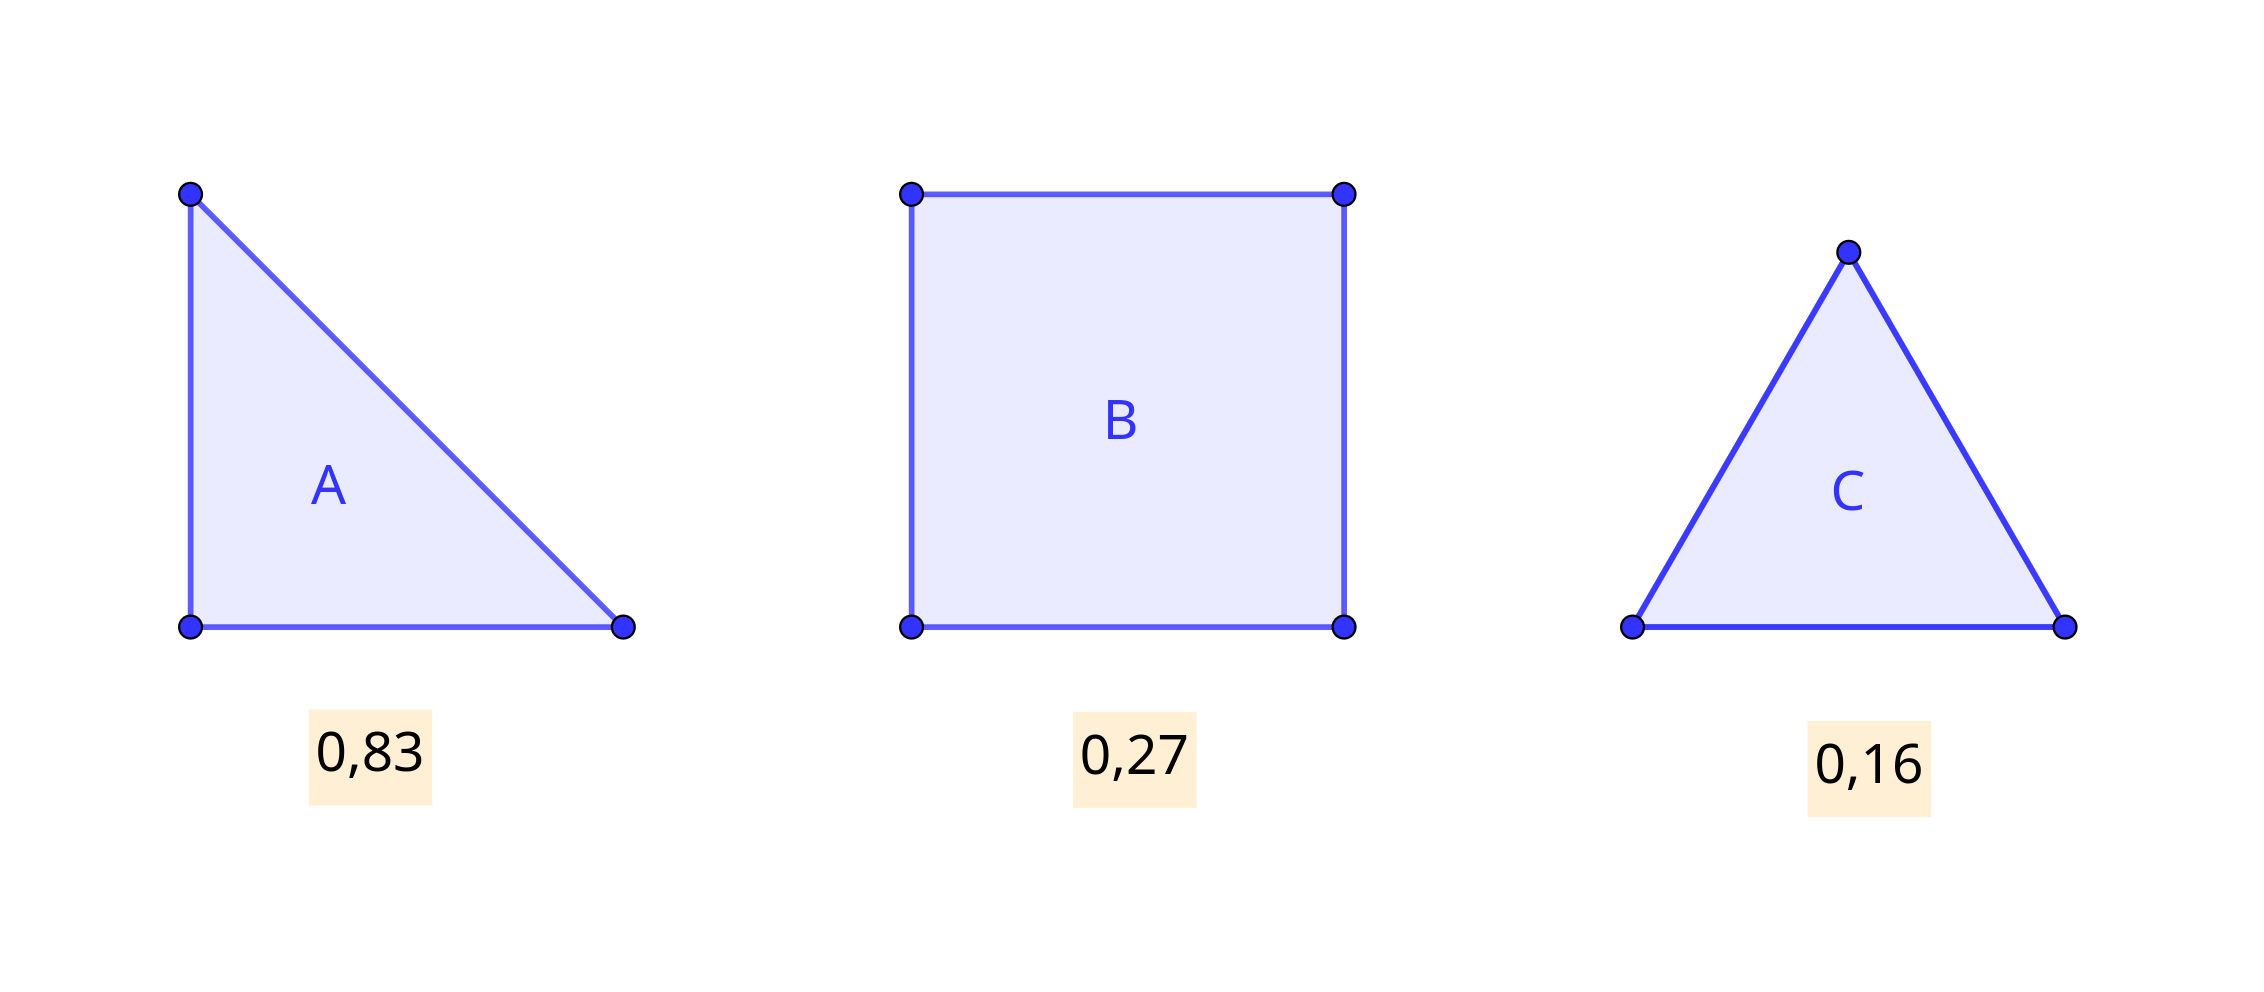
\includegraphics[width=0.58\linewidth]{imagens_brkga/ind1.png}
    \caption{Chaves aleatórias geradas para o primeiro indivíduo.}
    \label{fig:f14}
\end{figure}

\begin{figure}[H]
    \centering
    \begin{subfigure}{.58\textwidth}
        \centering
        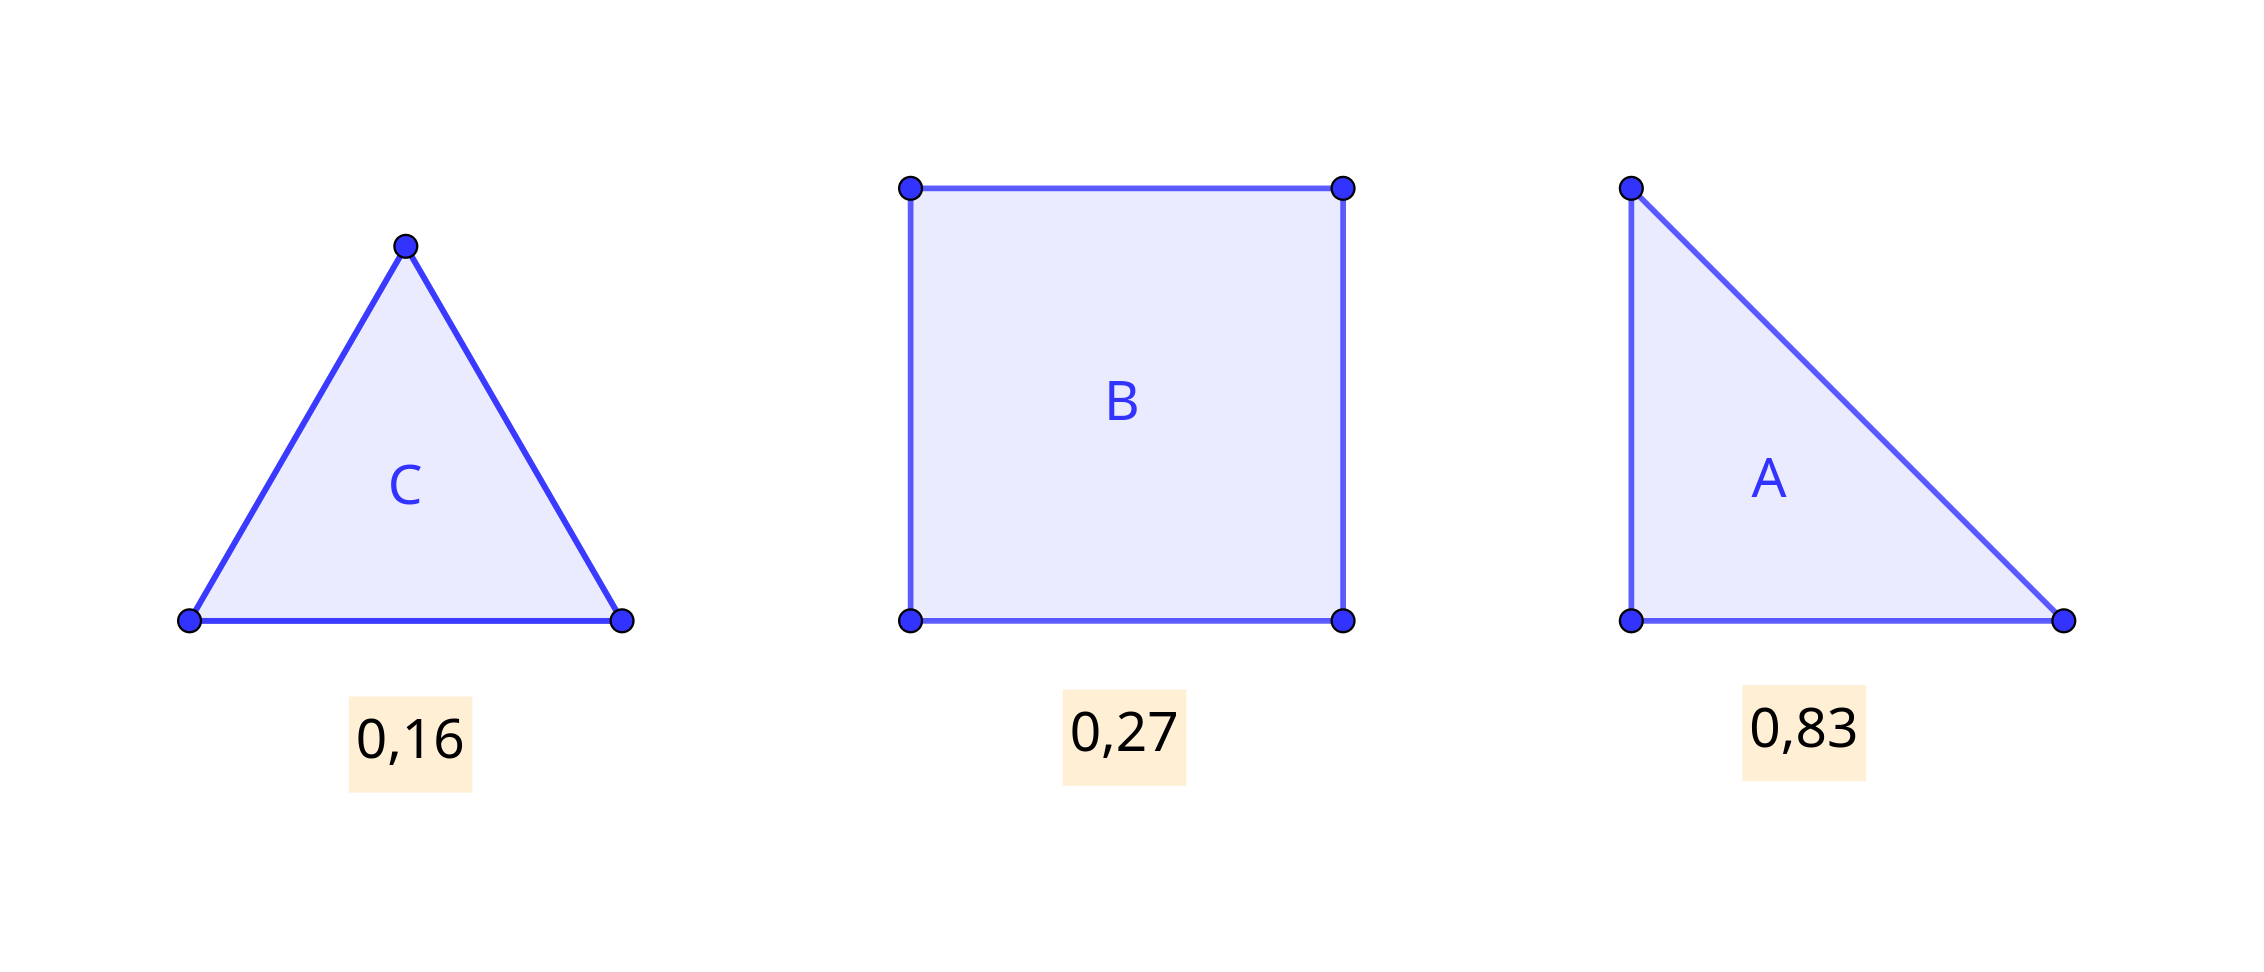
\includegraphics[width=\linewidth]{imagens_brkga/ind1_ord.png}
        \caption{}
        \label{fig:f15a}
    \end{subfigure}
    \hfill
    \begin{subfigure}{.33\textwidth}
        \centering
        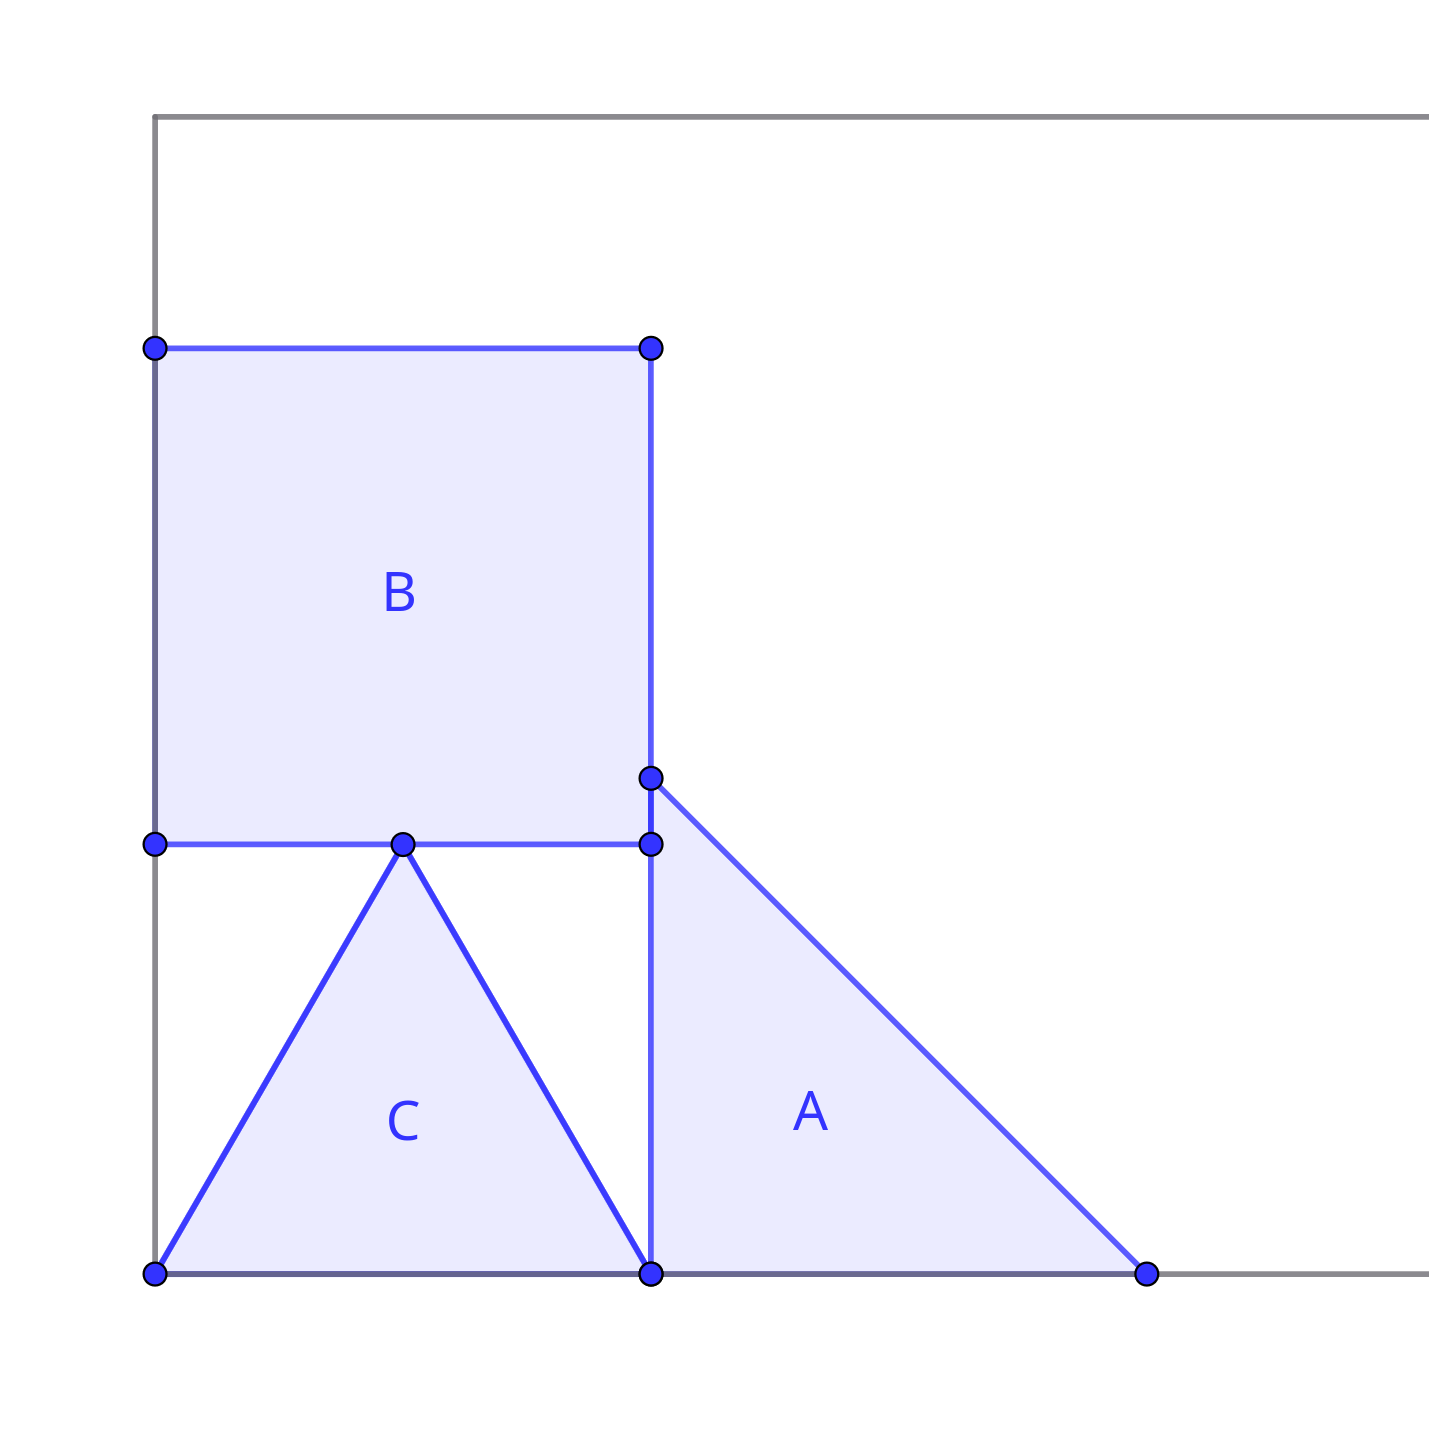
\includegraphics[width=\linewidth]{imagens_brkga/ind1_aloc.png}
        \caption{}
        \label{fig:f15b}
    \end{subfigure}
    \hfill
    \caption{Indivíduo $1$ ordenado conforme as chaves em ordem crescente em \,(a)\, e e sua alocação com base na {\it BL} seguindo tal ordenação em \,(b)\,.}
    \label{fig:f15}
\end{figure}

\begin{figure}[H]
    \centering
    \begin{subfigure}{.58\textwidth}
        \centering
        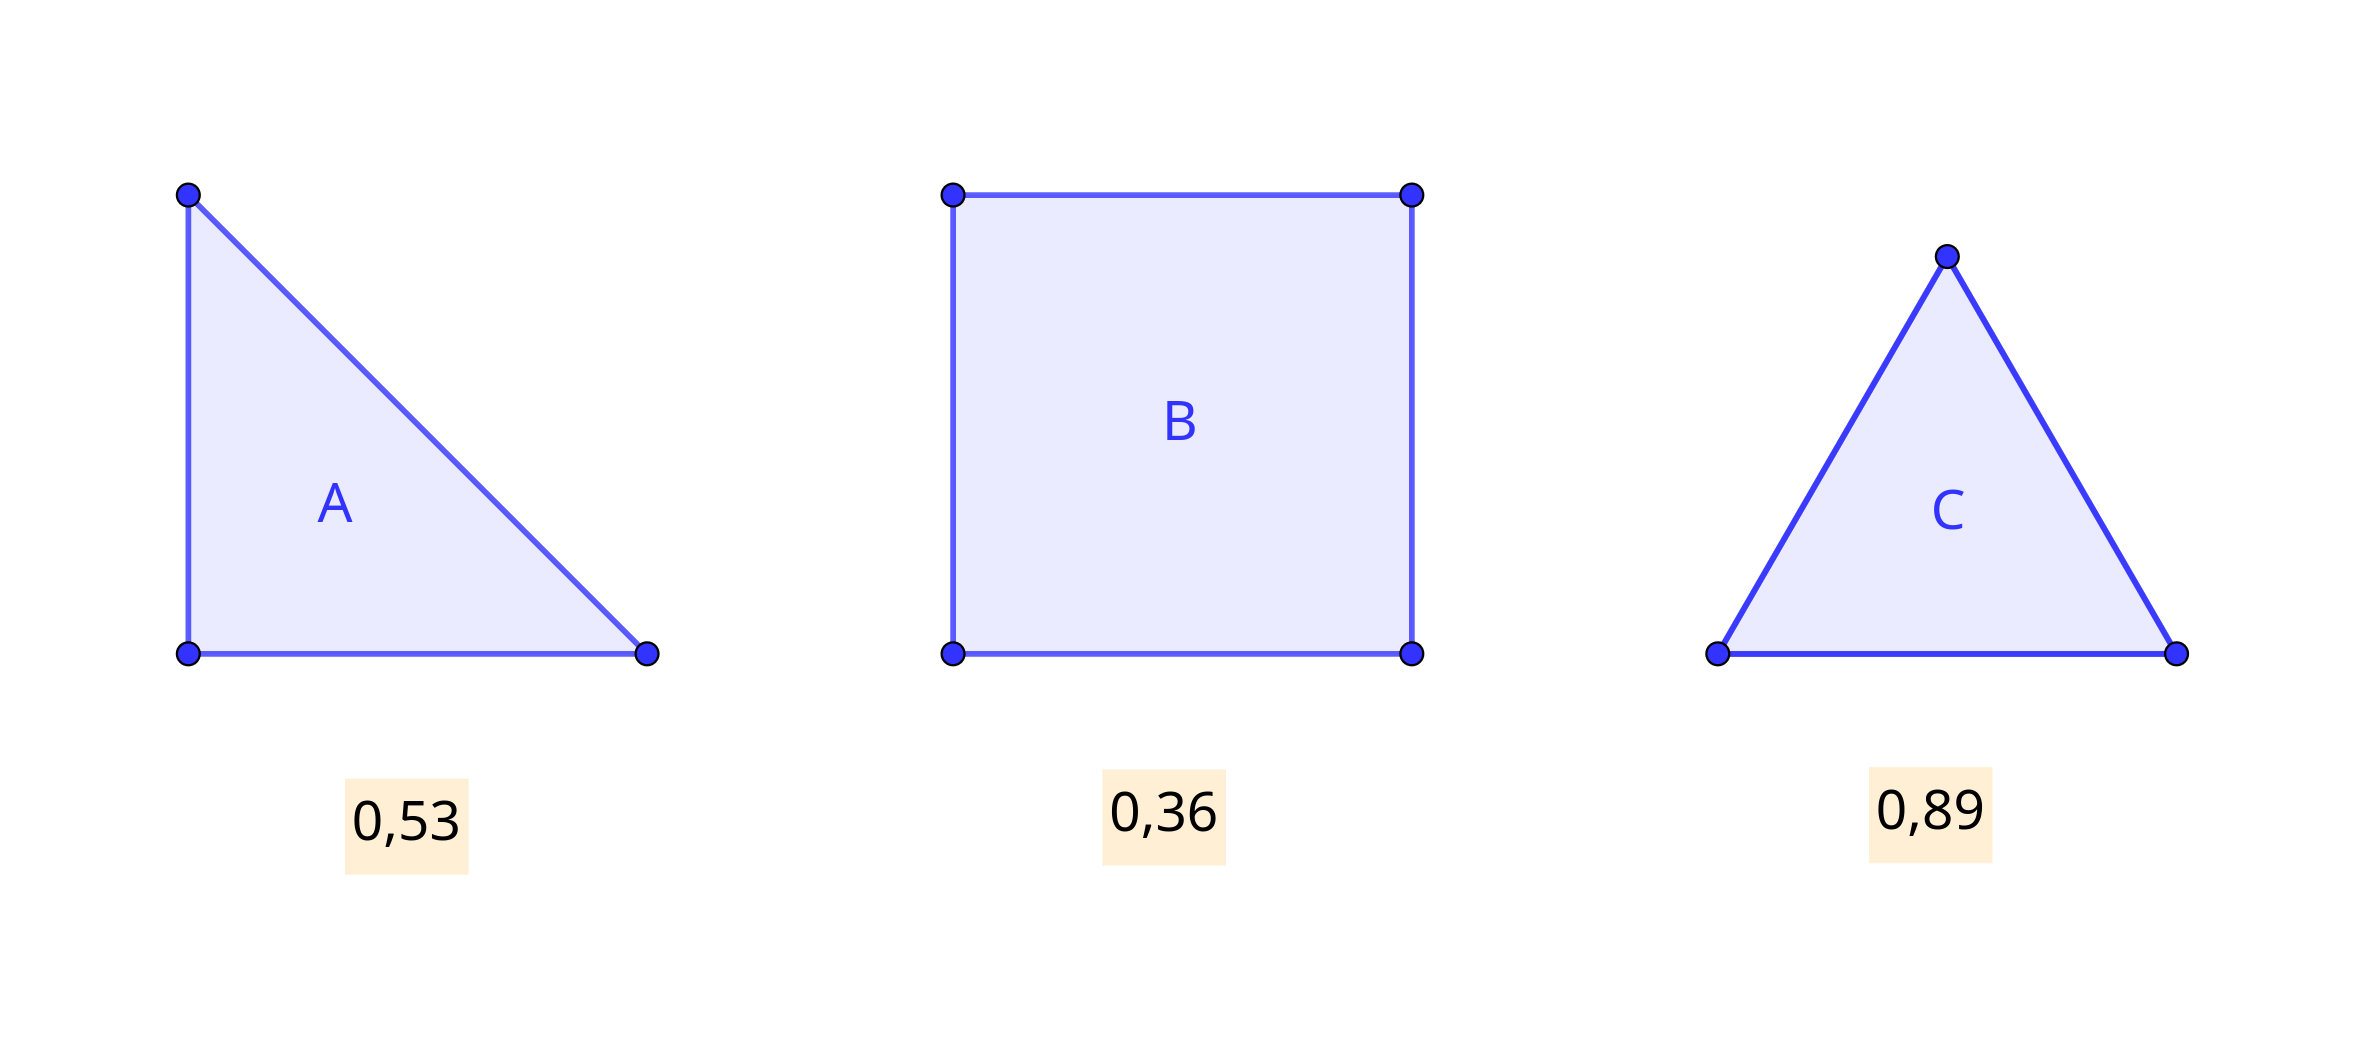
\includegraphics[width=\linewidth]{imagens_brkga/ind2.png}
        \caption{}
        \label{fig:f16a}
    \end{subfigure}
    \hfill
    \begin{subfigure}{.33\textwidth}
    \centering
        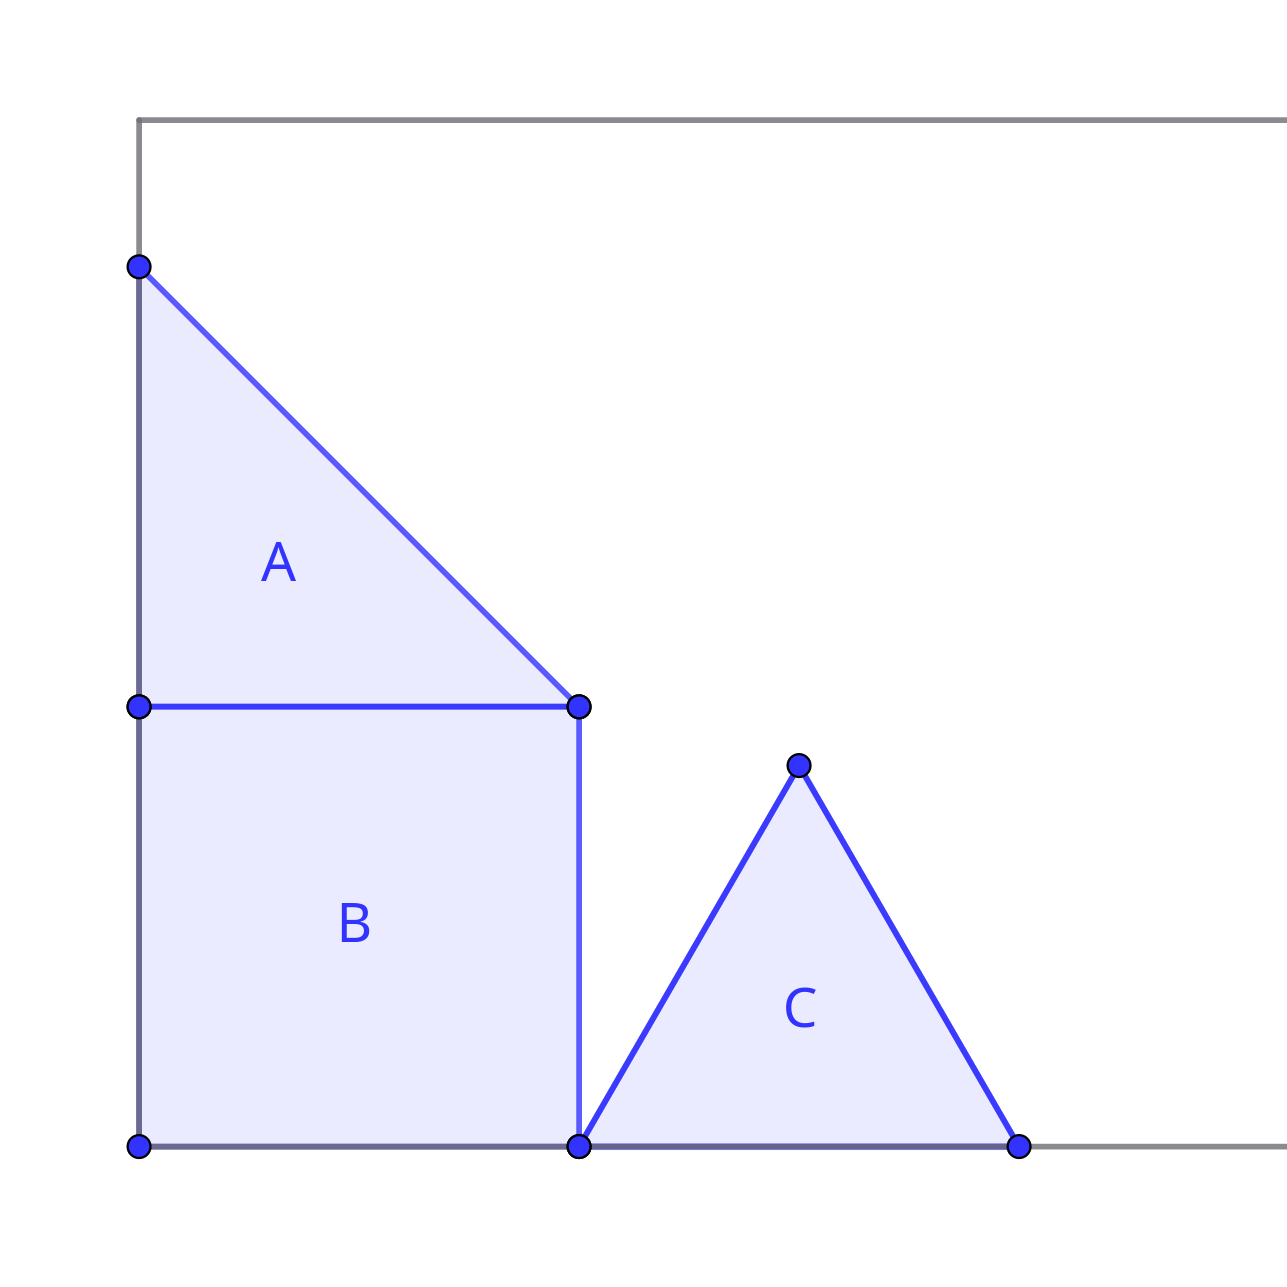
\includegraphics[width=\linewidth]{imagens_brkga/ind2_aloc.png}
        \caption{}
        \label{fig:f16b}
    \end{subfigure}
    \hfill
    \caption{Chaves do segundo indivíduo geradas em \,(a)\, e então sua alocação seguindo a {\it BL} após ordenar tais chaves, em \,(b)\,.}
    \label{fig:f16}
\end{figure}

Para exemplificar o cruzamento, usando o mesmo exemplo, o cromossomo de cada um dos pais é tomado em sua ordem original (ou seja, antes da ordenação de chaves) e para cada item do indivíduo novo é sorteado de qual indivíduo será proveniente a chave atrelada. Observe na Figura~\ref{fig:f17} o descendente $3$ criado a partir do cruzamento entre $1$ e $2$ e em~\ref{fig:f18} como fica então sua ordenação. Perceba que, embora os valores não sejam os mesmos, sua ordenação é a mesma do indivíduo $2$, ou seja, nem sempre o cruzamento gera indivíduos diferentes.

\begin{figure}[H]
    \centering
    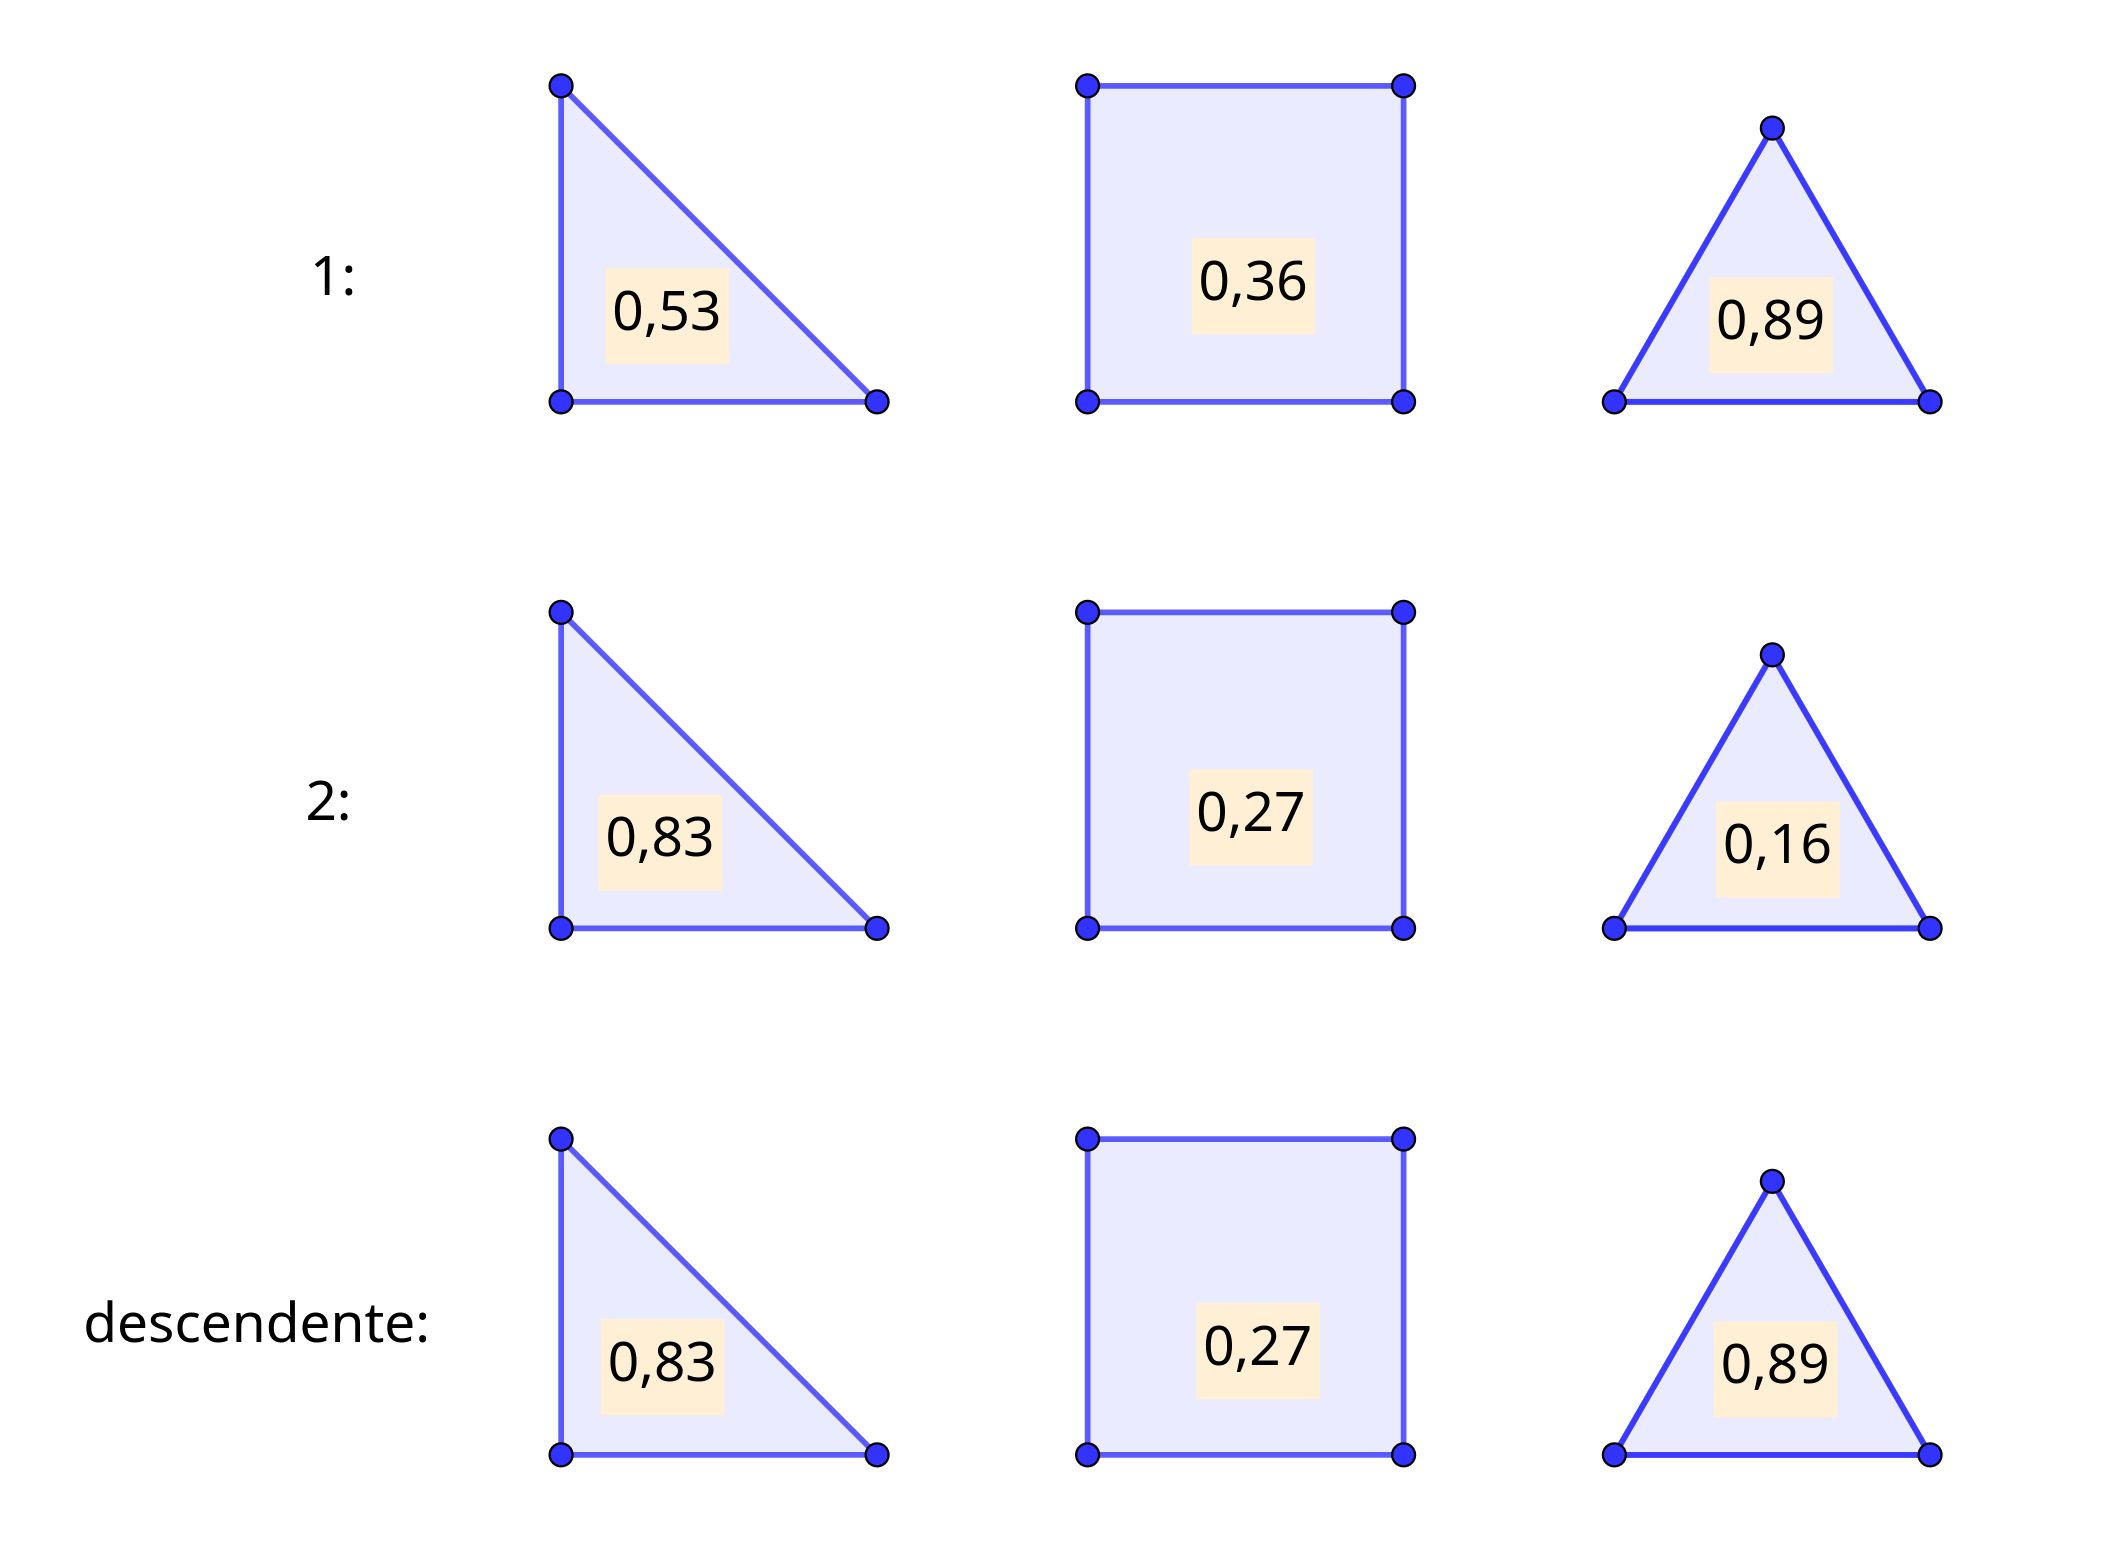
\includegraphics[width=0.58\linewidth]{imagens_brkga/cruzamento.png}
    \caption{Cruzamento entre indivíduos $1$ e $2$ gerando um descendente $3$.}
    \label{fig:f17}
\end{figure}

\begin{figure}[H]
    \centering
    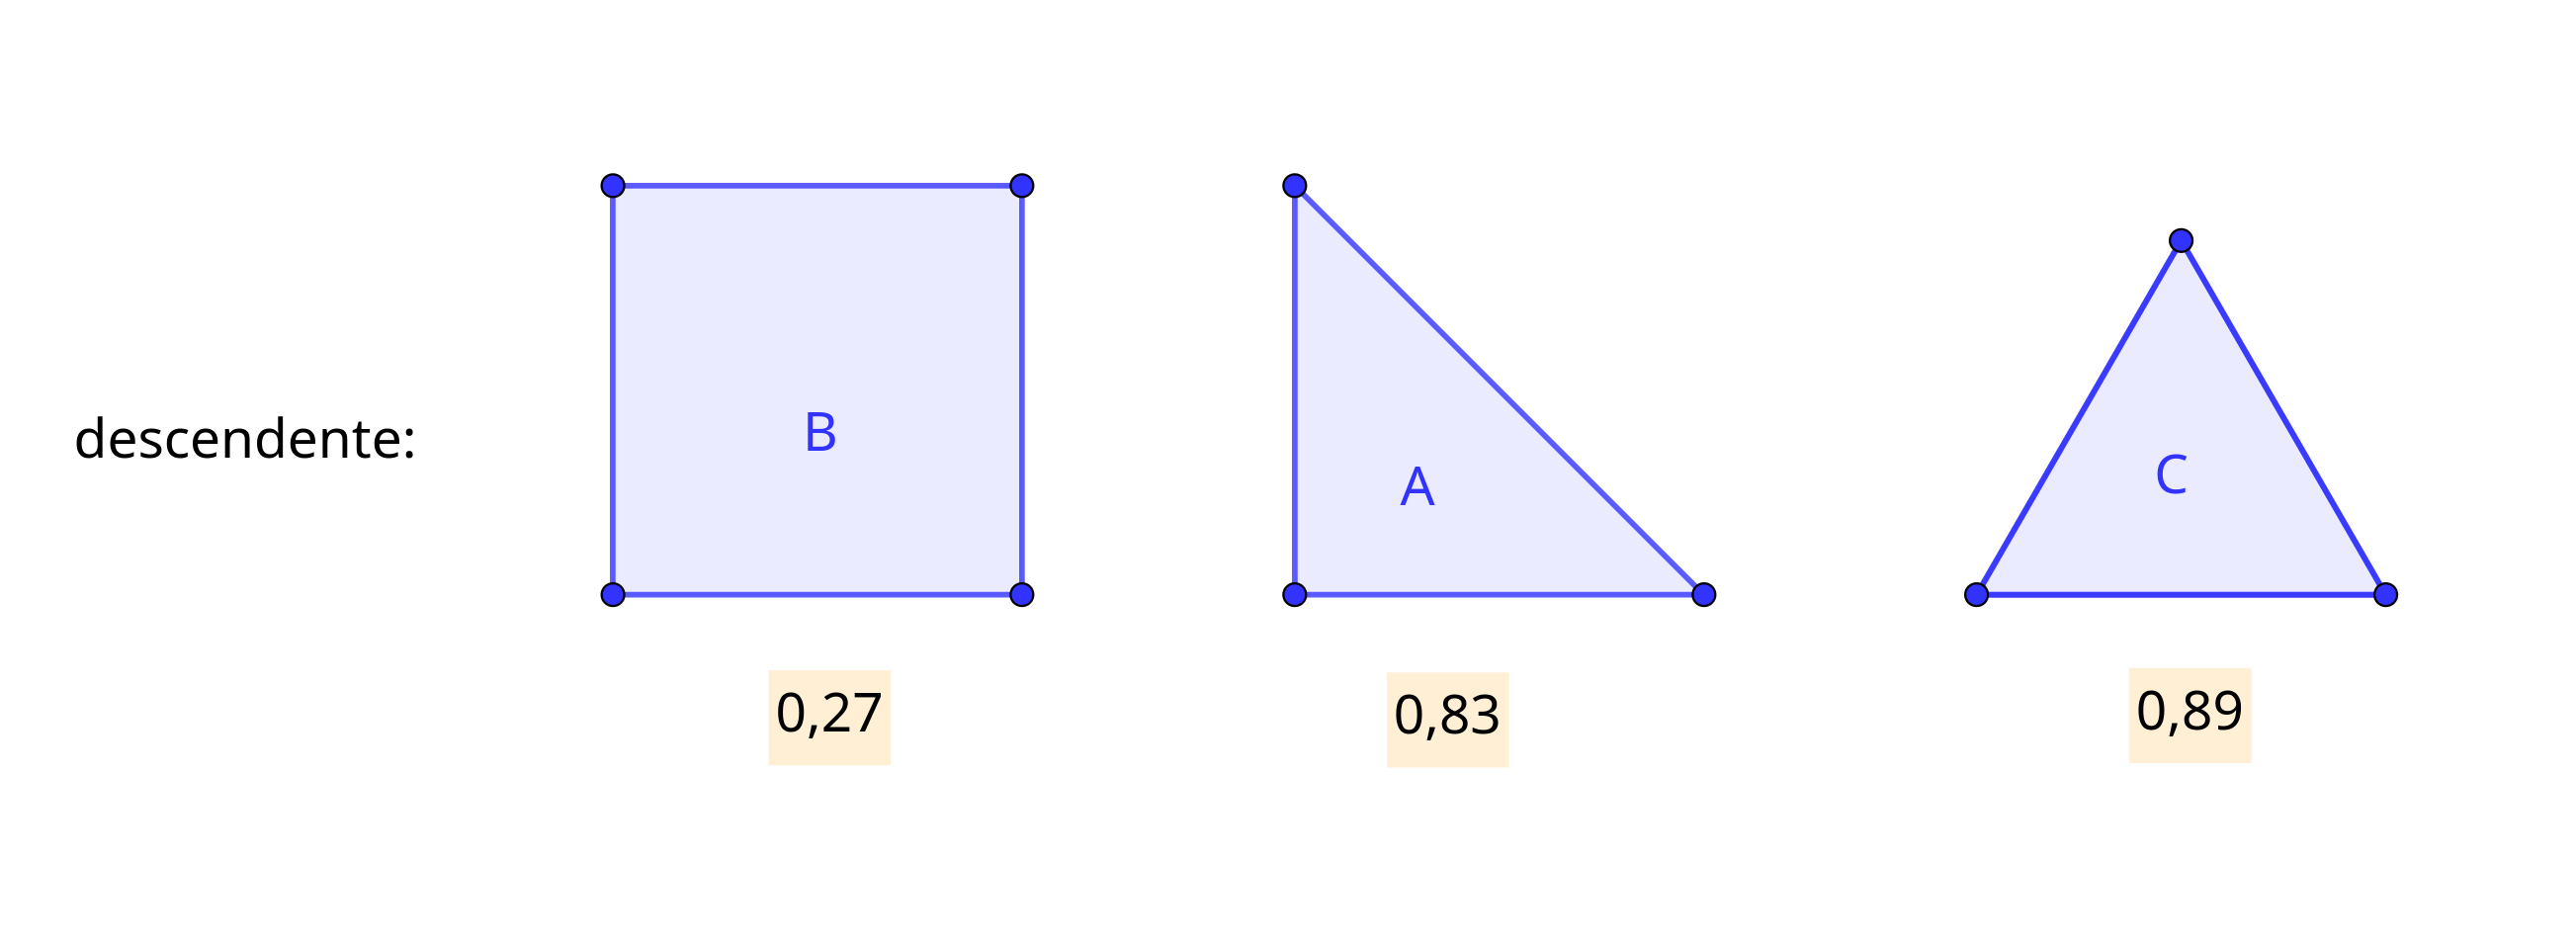
\includegraphics[width=0.68\linewidth]{imagens_brkga/desc.png}
    \caption{Ordenação final do descendente $3$, com chaves ordenadas em ordem crescente.}
    \label{fig:f18}
\end{figure}


Implementamos a {\it BRKGA} em linguagem C, com as mesmas especificações de leitura feitas para a implementação da {\it BL}, especificadas na Seção~\ref{sec:BL}.%, porém ao invés de um arquivo ``makefile'' utilizado para a execução, é utilizado um arquivo ``comando.sh'' onde cada linha é o comando de execução com a instância a ser rodada e 
Os valores dos parâmetros $I$, $G$, $E$, $C$ e $b$ são passados para o programa no momento de sua execução. A estrutura de dados dos itens e {\it NFPs} também é a mesma apresentada na implementação da {\it BL}.

Em relação à estrutura de dados específica para o algoritmo genético, temos a população que armazena os valores referentes à quantidade de indivíduos $E$ da elite, $M$ da mutação e $C$ do cruzamento, o viés $b$ do cruzamento, $G$ da quantidade de gerações totais, $I$ total de indivíduos na população, além de um ponteiro para o vetor fixo de indivíduos ao longo das gerações e um ponteiro para um vetor ``lixo'' de indivíduos, utilizado para armazenar os indivíduos provenientes do cruzamento antes de colocá-los no vetor fixo.

Cada indivíduo é composto pelo seu {\it fitness}, um ponteiro para um vetor que armazena as chaves na ordem original de criação e um ponteiro para vetor dos itens, em que cada um armazena o número $x$ de um item e a chave $k$ associada a ele.

Após a leitura dos dados, o programa passa pelas etapas a seguir:
%que na primeira geração $4$ indivíduos tiveram chaves específicas provenientes de bons resultados para a aplicação na {\it BL}, e os outros $I - 4$ tiveram as chaves geradas aleatoriamente. As soluções em específico escolhidas para compor a população como esses $4$ indivíduos foram as melhores das $12$ composições de método-ordenação para a {\it BL} citadas em~\ref{sec:experimentosbl}, dadas pela $BL_{31}$, $BL_{21}$, $BL_{52}$ e $BL_{11}$.

\begin{enumerate}
    \item Constrói a primeira geração de $I$ indivíduos, sendo que $4$ indivíduos tem suas chaves selecionadas a partir das melhores ordenações para a {\it BL} (aquelas citadas na Seção~\ref{sec:experimentosbl}, dadas pela $BL_{31}$, $BL_{21}$, $BL_{52}$ e $BL_{11}$), enquanto os outros $I-4$ tem as chaves geradas aleatoriamente;
    \item Para cada indivíduo $i$, $i = 1, \dots, I$:
    \begin{enumerate}
        \item Ordena o cromossomo de $i$;
        \item Chama a {\it BL}, obtendo o {\it fitness} $f$ de $i$;
    \end{enumerate}
    \item Para cada geração $g$, $g = 1, \dots, G$:
    \begin{enumerate}
        \item Ordena os $E$ melhores indivíduos a partir do valor do {\it fitness} na elite;
        \item Gera $C$ indivíduos a partir do cruzamento de indivíduos elite e não-elite;
        \item Mantém a elite da geração $g-1$ e substitui os não-elite pelos $C$ advindos do cruzamento;
        \item Completa a população com $M$ indivíduos novos gerados por mutação, com chaves aleatórias;
        \item Para cada indivíduo $i$, $i = 1, \dots, (C+M) = 1, \dots, (I-E)$:
        \begin{enumerate}
            \item Ordena o cromossomo de $i$;
            \item Aplica a {\it BL} para calcular o {\it fitness} de $i$;
        \end{enumerate}
    \end{enumerate}
\end{enumerate}

Por fim o programa identifica qual o indivíduo com melhor {\it fitness} resultante e imprime em um arquivo Latex a partir da ferramenta {\it Tikz} o leiaute correspondente, em que o recipiente é representado em azul, o comprimento obtido é a linha vertical pontilhada e os itens são coloridos (itens não convexos são representados por suas partes convexas conectadas, de mesma cor). Imprime também as informações de comprimento mínimo alcançado e tempo de execução num único arquivo de texto para facilitar sua disposição em forma de tabela (como a da Seção \ref{sec:experimentosbl}).


\subsection{Experimentos numéricos} \label{sec:experimentosBRKGA}

A meta-heurística {\it BRKGA} utilizou como parâmetros $I = 100$, $E = 20$, $M = 10$, $C = 70$ e $G = 10$. Para cada instância executamos o {\it BRKGA} duas vezes, uma com $b = 0,7$ e outra com $b = 0,5$. Os experimentos foram feitas usando as mesmas vinte e nove instâncias clássicas da literatura\footnote{\url{https://www.euro-online.org/websites/esicup/data-sets/}, acessado em 14/08/2025.} da Seção~\ref{sec:experimentosbl}, executadas também no mesmo computador presente nesta.

Os resultados obtidos se encontram na Tabela~\ref{tab:t3}. A coluna ``Instância'' contém o nome de cada instância utilizada, a ``Itens'' retrata o número de itens da instância (incluindo as cópias de cada item). Em seguida, os grupos de duas colunas apresentam os resultado de cada execução da {\it BRKGA}, uma com viés $0,5$ e a outra com viés $0,7$. A coluna ``Comp'' representa o comprimento obtido para a instância pela $BRKGA$ correspondente, em que o valor em destaque em cada linha é o menor resultado obtido e a coluna ``T(s)'' apresenta o tempo em segundos que a heurística levou para resolver cada instância.


\begin{adjustwidth}{-2 cm}{-2,5 cm}\centering\begin{threeparttable}[!htb]
\renewcommand{\arraystretch}{1.2}%
    \caption{Resultados obtidos pelas duas variações da meta-heurística $BRKGA$, com viés de $0,5$ e $0,7$.}
    \scriptsize{
        \begin{tabular}{|l|c|rr|rr|}\hline
        \multicolumn{1}{|c|}{} & \multicolumn{1}{c|}{} &  \multicolumn{2}{c|}{$BRKGA$ - viés $0,5$} & \multicolumn{2}{c|}{$BRKGA$ - viés $0,7$}\\
        Instância &Itens &Comp &T (s) &Comp &T (s) \\\hline
        albano &24 &\lgray10768,74 &674,09 &10878,59 &637,40 \\
        blaze1 &28 &28,67 &405,20 &\lgray27,87 &402,13 \\
        blaze2 &16 &21,23 &86,83 &\lgray21,13 &87,11 \\
        dagli &30 &66,12 &597,12 &\lgray65,17 &655,30 \\
        dighe1 &16 &133,72 &6,79 &\lgray133,02 &6,69 \\
        dighe2 &10 &\lgray129,70 &2,33 &132,87 &2,31 \\
        fu &12 &35,97 &1,85 &\lgray35,14 &1,69 \\
        jakobs1 &25 &\lgray12,00 &108,46 &\lgray12,00 &111,80 \\
        jakobs2 &25 &28,00 &220,78 &\lgray27,50 &216,67 \\
        mao &20 &\lgray2031,75 &977,08 &2032,92 &982,93 \\
        marques &24 &84,75 &477,07 &\lgray83,00 &483,63 \\
        poly1A &15 &16,57 &19,08 &\lgray16,51 &18,22 \\
        poly2A &30 &\lgray31,90 &163,26 &31,96 &165,36 \\
        poly2b &30 &34,25 &201,48 &\lgray33,96 &199,96 \\
        poly3A &45 &\lgray47,06 &573,20 &47,15 &580,47 \\
        poly3b &45 &45,29 &691,01 &\lgray44,29 &681,84 \\
        poly4A &60 &\lgray62,36 &1353,01 &62,49 &1381,14 \\
        poly4b &60 &55,97 &1490,48 &\lgray55,79 &1497,29 \\
        poly5A &75 &\lgray77,10 &2624,35 &77,57 &2655,93 \\
        poly5b &75 &67,22 &2874,35 &\lgray67,07 &2847,81 \\
        shapes0 &43 &64,75 &9090,53 &\lgray64,00 &9049,48 \\
        shapes1 &43 &\lgray65,00 &9094,61 &\lgray65,00 &9295,66 \\
        shirts &99 &65,37 &15331,76 &\lgray64,77 &14867,72 \\
        three &3 &\lgray6,20 &0,04 &\lgray6,20 &0,05 \\
        threep2 &6 &\lgray9,33 &0,33 &\lgray9,33 &0,31 \\
        threep2w9 &6 &\lgray8,50 &0,31 &\lgray8,50 &0,32 \\
        threep3 &9 &14,00 &1,04 &\lgray13,53 &1,03 \\
        threep3w9 &9 &11,25 &1,09 &\lgray11,10 &0,97 \\
        trousers &64 &\lgray269,33 &3789,94 &271,47 &3627,32 \\
        \hline
        \end{tabular}
    }
    \label{tab:t3}
\end{threeparttable}\end{adjustwidth}


\vspace{15pt}


Os resultados nos levam a acreditar que o viés de $0,7$ aplicado no cruzamento entre indivíduos, ou seja, enviesar o resultado para aumentar a probabilidade de que cada chave do novo cromossomo proceda do indivíduo elite escolhido, obtém melhores soluções, ao menos para as instâncias apresentadas.


\section{Comparação entre métodos utilizados} \label{sec:comp}

A seguir, na Tabela~\ref{tab:t4} temos a comparação entre os dois resultados da {\it BRKGA} e os quatro melhores da {\it BL}. A coluna ``Instância'' contém o nome de cada instância utilizada, a ``Itens'' retrata o número de itens da instância (incluindo as cópias de cada item). Em seguida, os grupos de duas colunas apresentam os resultado de cada execução com o respectivo método utilizado no topo da coluna. A coluna ``Comp'' representa o comprimento obtido para a instância pela heurística correspondente, em que o valor em destaque em cada linha é o menor resultado obtido e a coluna ``T(s)'' apresenta o tempo em segundos que a heurística levou para resolver cada instância.

%\textcolor{red}{ATÉ AGORA ESTAVA FALANDO EM COMPRIMENTO, MAS A PARTIR DAQUI VIROU . DEIXA TUDO IGUAL.}

É possível perceber que em todas as instâncias o comprimento final obtida pela {\it BRKGA} foi melhor que todas da {\it BL} apresentadas, incluindo as outras oito variações que se encontram nas tabelas~\ref{tab:t1} e~\ref{tab:t2}. O único caso em que o resultado da {\it BRKGA} é igual a algum da {\it BL} é a instância {\it Three}, cuja solução $6,20$ já tinha sido obtida pela $BL_{12}$. Ainda assim, em muitos casos essa diferença é muito pequena e, ao levar em conta o fato de que o custo computacional e de tempo da {\it BRKGA} é em média 1500 vezes maior que os da {\it BL}, não é necessariamente recomendado seu uso.

\begin{adjustwidth}{-2.5 cm}{-2.5 cm}\centering\begin{threeparttable}[!htb]
\renewcommand{\arraystretch}{1.2}%
    \caption{Resultados obtidos pelas duas variações da $BRKGA$ e os quatro melhores da $BL$.}
    \scriptsize{
    \begin{tabular}{|l|c|rr|rr|rr|rr|rr|rr|}\hline
        \multicolumn{1}{|c|}{} & \multicolumn{1}{c|}{} &\multicolumn{2}{c|}{$BRKGA$ - bias $0.5$} &\multicolumn{2}{c|}{$BRKGA$ - bias $0.7$} &\multicolumn{2}{c|}{$BL_{31}$} &\multicolumn{2}{c|}{$BL_{21}$} &\multicolumn{2}{c|}{$BL_{52}$} &\multicolumn{2}{c|}{$BL_{11}$} \\
        Instância & Itens &Comp &T (s) &Comp &T (s) &Comp &T (s) &Comp &T (s) &Comp &T (s) &Comp &T (s) \\\hline
        albano &24 &\lgray10768.74 &674.09 &10878.59 &637.40 &11376.46 &0.42 &11818.58 &0.29 &13525.12 &0.36 &11818.58 &0.37 \\
        blaze1 &28 &28.67 &405.20 &\lgray27.87 &402.13 &28.67 &0.22 &31.20 &0.20 &34.34 &0.21 &30.35 &0.28 \\
        blaze2 &16 &21.23 &86.83 &\lgray21.13 &87.11 &21.50 &0.08 &22.10 &0.06 &25.29 &0.04 &21.50 &0.09 \\
        dagli &30 &66.12 &597.12 &\lgray65.17 &655.30 &75.47 &0.57 &73.33 &0.39 &89.92 &0.23 &67.69 &0.43 \\
        dighe1 &16 &133.72 &6.79 &\lgray133.02 &6.69 &146.96 &0.00 &167.06 &0.00 &165.75 &0.00 &163.26 &0.00 \\
        dighe2 &10 &\lgray129.70 &2.33 &132.87 &2.31 &145.56 &0.00 &163.23 &0.00 &165.16 &0.00 &154.30 &0.00 \\
        fu &12 &35.97 &1.85 &\lgray35.14 &1.69 &42.25 &0.00 &36.46 &0.00 &43.46 &0.00 &42.00 &0.00 \\
        jakobs1 &25 &\lgray12.00 &108.46 &\lgray12.00 &111.80 &14.00 &0.10 &13.00 &0.08 &17.00 &0.06 &13.00 &0.09 \\
        jakobs2 &25 &28.00 &220.78 &\lgray27.50 &216.67 &30.00 &0.21 &30.00 &0.17 &32.00 &0.17 &29.60 &0.16 \\
        mao &20 &\lgray2031.75 &977.08 &2032.92 &982.93 &2119.63 &0.53 &2289.22 &0.46 &2509.27 &0.46 &2305.08 &0.46 \\
        marques &24 &84.75 &477.07 &\lgray83.00 &483.63 &89.60 &0.32 &87.00 &0.28 &96.00 &0.26 &93.10 &0.33 \\
        poly1A &15 &16.57 &19.07 &\lgray16.51 &18.22 &18.10 &0.01 &20.18 &0.01 &22.56 &0.01 &22.05 &0.01 \\
        poly2A &30 &\lgray31.94 &163.26 &31.96 &165.36 &33.33 &0.10 &32.31 &0.09 &40.14 &0.09 &36.11 &0.11 \\
        poly2b &30 &34.25 &201.48 &\lgray33.96 &199.96 &35.25 &0.12 &35.96 &0.11 &41.01 &0.11 &37.07 &0.13 \\
        poly3A &45 &\lgray47.06 &573.20 &47.15 &580.47 &50.08 &0.39 &52.28 &0.35 &56.83 &0.31 &53.63 &0.38 \\
        poly3b &45 &45.29 &691.00 &\lgray44.29 &681.84 &45.68 &0.45 &45.29 &0.35 &51.14 &0.34 &48.42 &0.46 \\
        poly4A &60 &\lgray62.36 &1353.01 &62.49 &1381.14 &66.52 &0.86 &66.96 &0.82 &68.35 &0.73 &69.11 &0.95 \\
        poly4b &60 &55.97 &1490.47 &\lgray55.79 &1497.29 &55.97 &0.91 &56.99 &0.85 &61.77 &0.82 &60.25 &0.96 \\
        poly5A &75 &\lgray77.10 &2624.35 &77.57 &2655.93 &80.06 &1.74 &80.39 &1.55 &85.44 &1.48 &82.98 &1.95 \\
        poly5b &75 &67.22 &2874.35 &\lgray67.07 &2847.80 &69.28 &1.81 &67.52 &1.50 &70.99 &1.52 &71.56 &1.85 \\
        shapes0 &43 &64.75 &9090.53 &\lgray64.00 &9049.48 &67.00 &7.26 &68.50 &5.92 &66.00 &4.59 &68.50 &6.04 \\
        shapes1 &43 &\lgray65.00 &9094.61 &\lgray65.00 &9295.66 &67.00 &6.83 &68.50 &5.89 &66.00 &4.60 &68.50 &5.68 \\
        shirts &99 &65.37 &15331.76 &\lgray64.77 &14867.72 &68.56 &7.76 &68.04 &7.71 &67.05 &7.96 &68.04 &7.63 \\
        three &3 &\lgray6.20 &0.04 &\lgray6.20 &0.05 &7.00 &0.00 &7.00 &0.00 &7.00 &0.00 &6.67 &0.00 \\
        threep2 &6 &\lgray9.33 &0.33 &\lgray9.33 &0.31 &10.00 &0.00 &10.00 &0.00 &10.00 &0.00 &10.67 &0.00 \\
        threep2w9 &6 &\lgray8.50 &0.31 &\lgray8.50 &0.32 &9.27 &0.00 &9.27 &0.00 &9.27 &0.00 &9.67 &0.00 \\
        threep3 &9 &14.00 &1.04 &\lgray13.53 &1.03 &16.33 &0.00 &16.33 &0.00 &16.33 &0.00 &16.33 &0.00 \\
        threep3w9 &9 &11.25 &1.09 &\lgray11.10 &0.97 &14.00 &0.00 &14.00 &0.00 &14.00 &0.00 &12.17 &0.00 \\
        trousers &64 &\lgray269.33 &3789.94 &271.47 &3627.32 &281.21 &1.63 &283.60 &1.98 &305.89 &2.01 &283.60 &1.90 \\
        \hline
    \end{tabular}
    }
    \label{tab:t4}
\end{threeparttable}\end{adjustwidth}

\vspace{15pt}


Observe nas figuras~\ref{fig:f11},~\ref{fig:f12},~\ref{fig:extra},~\ref{fig:f13} e~\ref{fig:f20} os leiautes obtidos na melhor e na pior alocação para a instância {\it fu} pela {\it BL}, a alocação desta obtida pela {\it BRKGA}, a melhor alocação obtida pela {\it BL} para a instância {\it blaze1} e a alocação desta pela {\it BRKGA}, com os respectivos comprimentos finais.

O exemplo utilizado na Seção~\ref{sec:irregular} ao explicar o problema, a Figura~\ref{fig:f1}, é o pior leiaute obtido para a instância {\it blaze1}, com comprimento final 36,92 e ordenação dos itens baseada na heurística $BL_{32}$ (ordenados de forma crescente pelo comprimento de cada item).


\begin{figure}[H]
    %\centering
    \begin{center}
    \hspace{0.24cm}
    \begin{tikzpicture}[scale=0.08]
          % item 0 copia 0 
        \filldraw [fill= \corA]  (20.263,23.882) -- (34.737,23.882) -- (34.737,38.355) -- (20.263,38.355) -- cycle;
        
          % item 0 copia 1 
        \filldraw [fill= \corB]  (34.737,23.882) -- (49.211,23.882) -- (49.211,38.355) -- (34.737,38.355) -- cycle;
        
          % item 2 copia 0 
        \filldraw [fill= \corC]  (14.474,40.526) -- (34.737,40.526) -- (34.737,53.553) -- (14.474,53.553) -- cycle;
        
          % item 3 copia 0 
        \filldraw [fill= \corD]  (32.505,13.750) -- (52.769,13.750) -- (42.637,23.882) -- cycle;
        
          % item 4 copia 0 
        \filldraw [fill= \corE]  (20.263,23.882) -- (20.263,10.855) -- (40.526,23.882) -- cycle;
        
          % item 5 copia 0 
        \filldraw [fill= \corF]  (0.000,0.000) -- (20.263,0.000) -- (20.263,20.263) -- (0.000,20.263) -- cycle;
        
          % item 6 copia 0 
        \filldraw [fill= \corG]  (34.737,38.355) -- (49.211,44.145) -- (49.211,51.382) -- (34.737,51.382) -- cycle;
        
          % item 7 copia 0 
        \filldraw [fill= \corH]  (44.688,0.000) -- (51.924,0.000) -- (51.924,13.026) -- (44.688,13.026) -- cycle;
        
          % item 8 copia 0 
        \filldraw [fill= \corI]  (0.000,20.263) -- (20.263,20.263) -- (20.263,40.526) -- cycle;
        
          % item 9 copia 0 
        \filldraw [fill= \corJ]  (0.000,34.737) -- (14.474,34.737) -- (14.474,49.211) -- (0.000,55.000) -- cycle;
        
          % item 10 copia 0 
        \filldraw [fill= \corK]  (33.470,13.750) -- (39.260,2.171) -- (45.049,13.750) -- cycle;
        
          % item 11 copia 0 
        \filldraw [fill= \corL]  (20.263,0.000) -- (40.526,0.000) -- (30.395,17.368) -- cycle;
        
           \draw[blue, very thick] (63.32, 0) -- (0,0) -- (0,55.00) -- (63.32, 55.00);
        
           \draw[dotted, very thick] (52.77, 0) -- (52.77,55.00);
    \end{tikzpicture}
    \end{center}
    \caption{Melhor resultado da instância {\it fu} pela {\it BL} (comprimento 36,46), obtido pela $BL_{21}$.}
    \label{fig:f11}
\end{figure}


\begin{figure}[H]
    %\centering
    %\vspace{2cm}
    \hspace{4.86cm}
    \begin{tikzpicture}[scale = 0.089]
          % item 0 copia 0 
        \filldraw [fill= \corA]  (18.054,9.081) -- (31.027,9.081) -- (31.027,22.054) -- (18.054,22.054) -- cycle;
        
          % item 0 copia 1 
        \filldraw [fill= \corB]  (28.865,22.054) -- (41.838,22.054) -- (41.838,35.027) -- (28.865,35.027) -- cycle;
        
          % item 2 copia 0 
        \filldraw [fill= \corC]  (28.865,35.027) -- (47.027,35.027) -- (47.027,46.703) -- (28.865,46.703) -- cycle;
        
          % item 3 copia 0 
        \filldraw [fill= \corD]  (0.000,22.054) -- (18.162,22.054) -- (9.081,31.135) -- cycle;
        
          % item 4 copia 0 
        \filldraw [fill= \corE]  (0.000,36.973) -- (0.000,25.297) -- (18.162,36.973) -- cycle;
        
          % item 5 copia 0 
        \filldraw [fill= \corF]  (41.838,13.838) -- (60.000,13.838) -- (60.000,32.000) -- (41.838,32.000) -- cycle;
        
          % item 6 copia 0 
        \filldraw [fill= \corG]  (0.000,36.973) -- (12.973,42.162) -- (12.973,48.649) -- (0.000,48.649) -- cycle;
        
          % item 7 copia 0 
        \filldraw [fill= \corH]  (0.000,10.378) -- (6.486,10.378) -- (6.486,22.054) -- (0.000,22.054) -- cycle;
        
          % item 8 copia 0 
        \filldraw [fill= \corI]  (10.703,29.514) -- (28.865,29.514) -- (28.865,47.676) -- cycle;
        
          % item 9 copia 0 
        \filldraw [fill= \corJ]  (31.027,0.000) -- (44.000,0.000) -- (44.000,12.973) -- (31.027,18.162) -- cycle;
        
          % item 10 copia 0 
        \filldraw [fill= \corK]  (0.000,10.378) -- (5.189,0.000) -- (10.378,10.378) -- cycle;
        
          % item 11 copia 0 
        \filldraw [fill= \corL]  (5.189,0.000) -- (23.351,0.000) -- (14.270,15.568) -- cycle;
        
           \draw[blue, very thick] (72.00, 0) -- (0,0) -- (0,49.30) -- (72.00, 49.30);
        
           \draw[dotted, very thick] (60.00, 0) -- (60.00,49.30);
    \end{tikzpicture}
    \caption{Pior resultado da instância {\it fu} (comprimento 46,25), obtido pela $BL_{12}$.}
    \label{fig:f12}
\end{figure}

\begin{figure}[H]
    \centering
    \hspace{0cm}
    \begin{tikzpicture}[scale = 0.079]
          % item 0 copia 0 
        \filldraw [fill= \corA]  (20.263,20.263) -- (34.737,20.263) -- (34.737,34.737) -- (20.263,34.737) -- cycle;
        
          % item 0 copia 1 
        \filldraw [fill= \corB]  (34.737,0.000) -- (49.211,0.000) -- (49.211,14.474) -- (34.737,14.474) -- cycle;
        
          % item 2 copia 0 
        \filldraw [fill= \corC]  (0.000,40.526) -- (20.263,40.526) -- (20.263,53.553) -- (0.000,53.553) -- cycle;
        
          % item 3 copia 0 
        \filldraw [fill= \corD]  (30.602,16.128) -- (50.865,16.128) -- (40.733,26.259) -- cycle;
        
          % item 4 copia 0 
        \filldraw [fill= \corE]  (0.000,40.526) -- (0.000,27.500) -- (20.263,40.526) -- cycle;
        
          % item 5 copia 0 
        \filldraw [fill= \corF]  (0.000,0.000) -- (20.263,0.000) -- (20.263,20.263) -- (0.000,20.263) -- cycle;
        
          % item 6 copia 0 
        \filldraw [fill= \corG]  (36.305,41.974) -- (50.779,47.763) -- (50.779,55.000) -- (36.305,55.000) -- cycle;
        
          % item 7 copia 0 
        \filldraw [fill= \corH]  (40.526,26.259) -- (47.763,26.259) -- (47.763,39.286) -- (40.526,39.286) -- cycle;
        
          % item 8 copia 0 
        \filldraw [fill= \corI]  (0.000,20.263) -- (20.263,20.263) -- (20.263,40.526) -- cycle;
        
          % item 9 copia 0 
        \filldraw [fill= \corJ]  (20.263,0.000) -- (34.737,0.000) -- (34.737,14.474) -- (20.263,20.263) -- cycle;
        
          % item 10 copia 0 
        \filldraw [fill= \corK]  (19.539,55.000) -- (25.329,43.421) -- (31.118,55.000) -- cycle;
        
          % item 11 copia 0 
        \filldraw [fill= \corL]  (20.263,34.737) -- (40.526,34.737) -- (30.395,52.105) -- cycle;
        
           \draw[blue, very thick] (61.04, 0) -- (0,0) -- (0,55.00) -- (61.04, 55.00);
        
           \draw[dotted, very thick] (50.86, 0) -- (50.86,55.00);
        
    \end{tikzpicture}
    %escala = 1.447
    %tempo = 1.685s
    \caption{Melhor resultado da instância {\it fu} (comprimento 35,14), obtido pela $BRKGA$.}
    \label{fig:extra}
\end{figure}



\begin{figure}[H]
    \centering
    \hspace{0.27cm}
    \begin{tikzpicture}[scale = 0.16]
          % item 0 copia 0 
        \filldraw [fill= \corA]  (43.256,29.302) -- (47.442,31.395) -- (51.628,29.302) -- (51.628,23.023) -- (47.442,20.930) -- (43.256,23.023) -- cycle;
        
          % item 0 copia 1 
        \filldraw [fill= \corB]  (45.837,8.372) -- (50.023,10.465) -- (54.209,8.372) -- (54.209,2.093) -- (50.023,0.000) -- (45.837,2.093) -- cycle;
        
          % item 0 copia 2 
        \filldraw [fill= \corC]  (46.842,18.335) -- (51.028,20.428) -- (55.214,18.335) -- (55.214,12.056) -- (51.028,9.963) -- (46.842,12.056) -- cycle;
        
          % item 0 copia 3 
        \filldraw [fill= \corD]  (51.628,26.407) -- (55.814,28.500) -- (60.000,26.407) -- (60.000,20.128) -- (55.814,18.035) -- (51.628,20.128) -- cycle;
        
          % item 1 copia 0 
        \filldraw [fill= \corE]  (10.465,18.837) -- (16.744,16.744) -- (18.837,12.558) -- (18.837,10.465) -- (14.651,10.465) -- (10.465,14.651) -- cycle;
        
          % item 1 copia 0 
        \filldraw [fill= \corE]  (10.465,18.837) -- (12.558,20.930) -- (18.837,20.930) -- (16.744,16.744) -- cycle;
        
          % item 1 copia 1 
        \filldraw [fill= \corF]  (10.465,29.302) -- (16.744,27.209) -- (18.837,23.023) -- (18.837,20.930) -- (14.651,20.930) -- (10.465,25.116) -- cycle;
        
          % item 1 copia 1 
        \filldraw [fill= \corF]  (10.465,29.302) -- (12.558,31.395) -- (18.837,31.395) -- (16.744,27.209) -- cycle;
        
          % item 1 copia 2 
        \filldraw [fill= \corG]  (17.791,18.837) -- (24.070,16.744) -- (26.163,12.558) -- (26.163,10.465) -- (21.977,10.465) -- (17.791,14.651) -- cycle;
        
          % item 1 copia 2 
        \filldraw [fill= \corG]  (17.791,18.837) -- (19.884,20.930) -- (26.163,20.930) -- (24.070,16.744) -- cycle;
        
          % item 1 copia 3 
        \filldraw [fill= \corH]  (17.791,29.302) -- (24.070,27.209) -- (26.163,23.023) -- (26.163,20.930) -- (21.977,20.930) -- (17.791,25.116) -- cycle;
        
          % item 1 copia 3 
        \filldraw [fill= \corH]  (17.791,29.302) -- (19.884,31.395) -- (26.163,31.395) -- (24.070,27.209) -- cycle;
        
          % item 2 copia 0 
        \filldraw [fill= \corI]  (23.023,8.372) -- (27.209,8.372) -- (29.302,6.279) -- (29.302,2.093) -- (27.209,0.000) -- (23.023,0.000) -- (20.930,2.093) -- (20.930,6.279) -- cycle;
        
          % item 2 copia 1 
        \filldraw [fill= \corJ]  (27.209,20.930) -- (31.395,20.930) -- (33.488,18.837) -- (33.488,14.651) -- (31.395,12.558) -- (27.209,12.558) -- (25.116,14.651) -- (25.116,18.837) -- cycle;
        
          % item 2 copia 2 
        \filldraw [fill= \corK]  (27.209,31.395) -- (31.395,31.395) -- (33.488,29.302) -- (33.488,25.116) -- (31.395,23.023) -- (27.209,23.023) -- (25.116,25.116) -- (25.116,29.302) -- cycle;
        
          % item 2 copia 3 
        \filldraw [fill= \corL]  (31.395,8.372) -- (35.581,8.372) -- (37.674,6.279) -- (37.674,2.093) -- (35.581,0.000) -- (31.395,0.000) -- (29.302,2.093) -- (29.302,6.279) -- cycle;
        
          % item 3 copia 0 
        \filldraw [fill= \corM]  (36.419,14.233) -- (32.233,12.140) -- (34.326,16.326) -- cycle;
        
          % item 3 copia 0 
        \filldraw [fill= \corM]  (36.419,20.512) -- (40.605,22.605) -- (38.512,18.419) -- cycle;
        
          % item 3 copia 0 
        \filldraw [fill= \corM]  (32.233,22.605) -- (36.419,20.512) -- (38.512,18.419) -- (40.605,12.140) -- (36.419,14.233) -- (34.326,16.326) -- cycle;
        
          % item 3 copia 1 
        \filldraw [fill= \corN]  (39.767,23.023) -- (35.581,20.930) -- (37.674,25.116) -- cycle;
        
          % item 3 copia 1 
        \filldraw [fill= \corN]  (39.767,29.302) -- (43.953,31.395) -- (41.860,27.209) -- cycle;
        
          % item 3 copia 1 
        \filldraw [fill= \corN]  (35.581,31.395) -- (39.767,29.302) -- (41.860,27.209) -- (43.953,20.930) -- (39.767,23.023) -- (37.674,25.116) -- cycle;
        
          % item 3 copia 2 
        \filldraw [fill= \corO]  (40.814,2.093) -- (36.628,0.000) -- (38.721,4.186) -- cycle;
        
          % item 3 copia 2 
        \filldraw [fill= \corO]  (40.814,8.372) -- (45.000,10.465) -- (42.907,6.279) -- cycle;
        
          % item 3 copia 2 
        \filldraw [fill= \corO]  (36.628,10.465) -- (40.814,8.372) -- (42.907,6.279) -- (45.000,0.000) -- (40.814,2.093) -- (38.721,4.186) -- cycle;
        
          % item 3 copia 3 
        \filldraw [fill= \corP]  (43.326,11.302) -- (39.140,9.209) -- (41.233,13.395) -- cycle;
        
          % item 3 copia 3 
        \filldraw [fill= \corP]  (43.326,17.581) -- (47.512,19.674) -- (45.419,15.488) -- cycle;
        
          % item 3 copia 3 
        \filldraw [fill= \corP]  (39.140,19.674) -- (43.326,17.581) -- (45.419,15.488) -- (47.512,9.209) -- (43.326,11.302) -- (41.233,13.395) -- cycle;
        
          % item 4 copia 0 
        \filldraw [fill= \corQ]  (6.279,4.186) -- (4.186,6.279) -- (10.465,10.465) -- cycle;
        
          % item 4 copia 0 
        \filldraw [fill= \corQ]  (4.186,6.279) -- (0.000,8.372) -- (0.000,10.465) -- (10.465,10.465) -- cycle;
        
          % item 4 copia 0 
        \filldraw [fill= \corQ]  (10.465,10.465) -- (10.465,0.000) -- (8.372,0.000) -- (6.279,4.186) -- cycle;
        
          % item 4 copia 1 
        \filldraw [fill= \corR]  (6.279,14.651) -- (4.186,16.744) -- (10.465,20.930) -- cycle;
        
          % item 4 copia 1 
        \filldraw [fill= \corR]  (4.186,16.744) -- (0.000,18.837) -- (0.000,20.930) -- (10.465,20.930) -- cycle;
        
          % item 4 copia 1 
        \filldraw [fill= \corR]  (10.465,20.930) -- (10.465,10.465) -- (8.372,10.465) -- (6.279,14.651) -- cycle;
        
          % item 4 copia 2 
        \filldraw [fill= \corS]  (6.279,25.116) -- (4.186,27.209) -- (10.465,31.395) -- cycle;
        
          % item 4 copia 2 
        \filldraw [fill= \corS]  (4.186,27.209) -- (0.000,29.302) -- (0.000,31.395) -- (10.465,31.395) -- cycle;
        
          % item 4 copia 2 
        \filldraw [fill= \corS]  (10.465,31.395) -- (10.465,20.930) -- (8.372,20.930) -- (6.279,25.116) -- cycle;
        
          % item 4 copia 3 
        \filldraw [fill= \corT]  (16.744,4.186) -- (14.651,6.279) -- (20.930,10.465) -- cycle;
        
          % item 4 copia 3 
        \filldraw [fill= \corT]  (14.651,6.279) -- (10.465,8.372) -- (10.465,10.465) -- (20.930,10.465) -- cycle;
        
          % item 4 copia 3 
        \filldraw [fill= \corT]  (20.930,10.465) -- (20.930,0.000) -- (18.837,0.000) -- (16.744,4.186) -- cycle;
        
          % item 5 copia 0 
        \filldraw [fill= \corU]  (4.186,6.279) -- (8.372,0.000) -- (0.000,0.000) -- cycle;
        
          % item 5 copia 1 
        \filldraw [fill= \corV]  (4.186,16.744) -- (8.372,10.465) -- (0.000,10.465) -- cycle;
        
          % item 5 copia 2 
        \filldraw [fill= \corW]  (4.186,27.209) -- (8.372,20.930) -- (0.000,20.930) -- cycle;
        
          % item 5 copia 3 
        \filldraw [fill= \corA]  (14.651,6.279) -- (18.837,0.000) -- (10.465,0.000) -- cycle;
        
          % item 6 copia 0 
        \filldraw [fill= \corB]  (26.163,12.558) -- (30.349,12.558) -- (30.349,8.372) -- (26.163,8.372) -- cycle;
        
          % item 6 copia 1 
        \filldraw [fill= \corC]  (54.209,4.186) -- (58.395,4.186) -- (58.395,0.000) -- (54.209,0.000) -- cycle;
        
          % item 6 copia 2 
        \filldraw [fill= \corD]  (54.209,8.372) -- (58.395,8.372) -- (58.395,4.186) -- (54.209,4.186) -- cycle;
        
          % item 6 copia 3 
        \filldraw [fill= \corE]  (55.214,12.558) -- (59.400,12.558) -- (59.400,8.372) -- (55.214,8.372) -- cycle;
        
           \draw[blue, very thick] (72.00, 0) -- (0,0) -- (0,31.40) -- (72.00, 31.40);
        
           \draw[dotted, very thick] (60.00, 0) -- (60.00,31.40);
    \end{tikzpicture}
    \caption{Melhor resultado da instância {\it blaze1} pela {\it BL} (comprimento 28,67), obtido pela $BL_{31}$.}
    \label{fig:f13}
\end{figure}


\begin{figure}[H]
    \begin{center}
    \hspace{0.01cm}
    \begin{tikzpicture}[scale = 0.156]
  % item 0 copia 0 
\filldraw [fill= \corA]  (34.306,29.856) -- (38.612,32.010) -- (42.919,29.856) -- (42.919,23.397) -- (38.612,21.244) -- (34.306,23.397) -- cycle;

  % item 0 copia 1 
\filldraw [fill= \corB]  (36.818,9.043) -- (41.124,11.196) -- (45.431,9.043) -- (45.431,2.584) -- (41.124,0.431) -- (36.818,2.584) -- cycle;

  % item 0 copia 2 
\filldraw [fill= \corC]  (41.483,19.809) -- (45.789,21.962) -- (50.096,19.809) -- (50.096,13.349) -- (45.789,11.196) -- (41.483,13.349) -- cycle;

  % item 0 copia 3 
\filldraw [fill= \corD]  (42.919,29.856) -- (47.225,32.010) -- (51.531,29.856) -- (51.531,23.397) -- (47.225,21.244) -- (42.919,23.397) -- cycle;

  % item 1 copia 0 
\filldraw [fill= \corE]  (10.766,19.378) -- (17.225,17.225) -- (19.378,12.919) -- (19.378,10.766) -- (15.072,10.766) -- (10.766,15.072) -- cycle;

  % item 1 copia 0 
\filldraw [fill= \corE]  (10.766,19.378) -- (12.919,21.531) -- (19.378,21.531) -- (17.225,17.225) -- cycle;

  % item 1 copia 1 
\filldraw [fill= \corF]  (10.766,30.144) -- (17.225,27.990) -- (19.378,23.684) -- (19.378,21.531) -- (15.072,21.531) -- (10.766,25.837) -- cycle;

  % item 1 copia 1 
\filldraw [fill= \corF]  (10.766,30.144) -- (12.919,32.297) -- (19.378,32.297) -- (17.225,27.990) -- cycle;

  % item 1 copia 2 
\filldraw [fill= \corG]  (18.301,19.378) -- (24.761,17.225) -- (26.914,12.919) -- (26.914,10.766) -- (22.608,10.766) -- (18.301,15.072) -- cycle;

  % item 1 copia 2 
\filldraw [fill= \corG]  (18.301,19.378) -- (20.455,21.531) -- (26.914,21.531) -- (24.761,17.225) -- cycle;

  % item 1 copia 3 
\filldraw [fill= \corH]  (18.301,30.144) -- (24.761,27.990) -- (26.914,23.684) -- (26.914,21.531) -- (22.608,21.531) -- (18.301,25.837) -- cycle;

  % item 1 copia 3 
\filldraw [fill= \corH]  (18.301,30.144) -- (20.455,32.297) -- (26.914,32.297) -- (24.761,27.990) -- cycle;

  % item 2 copia 0 
\filldraw [fill= \corI]  (23.684,8.612) -- (27.990,8.612) -- (30.144,6.459) -- (30.144,2.153) -- (27.990,0.000) -- (23.684,0.000) -- (21.531,2.153) -- (21.531,6.459) -- cycle;

  % item 2 copia 1 
\filldraw [fill= \corJ]  (27.990,21.531) -- (32.297,21.531) -- (34.450,19.378) -- (34.450,15.072) -- (32.297,12.919) -- (27.990,12.919) -- (25.837,15.072) -- (25.837,19.378) -- cycle;

  % item 2 copia 2 
\filldraw [fill= \corK]  (49.234,12.919) -- (53.541,12.919) -- (55.694,10.766) -- (55.694,6.459) -- (53.541,4.306) -- (49.234,4.306) -- (47.081,6.459) -- (47.081,10.766) -- cycle;

  % item 2 copia 3 
\filldraw [fill= \corL]  (52.249,21.531) -- (56.555,21.531) -- (58.708,19.378) -- (58.708,15.072) -- (56.555,12.919) -- (52.249,12.919) -- (50.096,15.072) -- (50.096,19.378) -- cycle;

  % item 3 copia 0 
\filldraw [fill= \corM]  (30.861,22.967) -- (26.555,20.813) -- (28.708,25.120) -- cycle;

  % item 3 copia 0 
\filldraw [fill= \corM]  (30.861,29.426) -- (35.167,31.579) -- (33.014,27.273) -- cycle;

  % item 3 copia 0 
\filldraw [fill= \corM]  (26.555,31.579) -- (30.861,29.426) -- (33.014,27.273) -- (35.167,20.813) -- (30.861,22.967) -- (28.708,25.120) -- cycle;

  % item 3 copia 1 
\filldraw [fill= \corN]  (33.373,2.153) -- (29.067,0.000) -- (31.220,4.306) -- cycle;

  % item 3 copia 1 
\filldraw [fill= \corN]  (33.373,8.612) -- (37.679,10.766) -- (35.526,6.459) -- cycle;

  % item 3 copia 1 
\filldraw [fill= \corN]  (29.067,10.766) -- (33.373,8.612) -- (35.526,6.459) -- (37.679,0.000) -- (33.373,2.153) -- (31.220,4.306) -- cycle;

  % item 3 copia 2 
\filldraw [fill= \corO]  (38.038,12.919) -- (33.732,10.766) -- (35.885,15.072) -- cycle;

  % item 3 copia 2 
\filldraw [fill= \corO]  (38.038,19.378) -- (42.344,21.531) -- (40.191,17.225) -- cycle;

  % item 3 copia 2 
\filldraw [fill= \corO]  (33.732,21.531) -- (38.038,19.378) -- (40.191,17.225) -- (42.344,10.766) -- (38.038,12.919) -- (35.885,15.072) -- cycle;

  % item 3 copia 3 
\filldraw [fill= \corP]  (55.024,23.684) -- (50.718,21.531) -- (52.871,25.837) -- cycle;

  % item 3 copia 3 
\filldraw [fill= \corP]  (55.024,30.144) -- (59.330,32.297) -- (57.177,27.990) -- cycle;

  % item 3 copia 3 
\filldraw [fill= \corP]  (50.718,32.297) -- (55.024,30.144) -- (57.177,27.990) -- (59.330,21.531) -- (55.024,23.684) -- (52.871,25.837) -- cycle;

  % item 4 copia 0 
\filldraw [fill= \corQ]  (6.459,4.306) -- (4.306,6.459) -- (10.766,10.766) -- cycle;

  % item 4 copia 0 
\filldraw [fill= \corQ]  (4.306,6.459) -- (0.000,8.612) -- (0.000,10.766) -- (10.766,10.766) -- cycle;

  % item 4 copia 0 
\filldraw [fill= \corQ]  (10.766,10.766) -- (10.766,0.000) -- (8.612,0.000) -- (6.459,4.306) -- cycle;

  % item 4 copia 1 
\filldraw [fill= \corR]  (6.459,15.072) -- (4.306,17.225) -- (10.766,21.531) -- cycle;

  % item 4 copia 1 
\filldraw [fill= \corR]  (4.306,17.225) -- (0.000,19.378) -- (0.000,21.531) -- (10.766,21.531) -- cycle;

  % item 4 copia 1 
\filldraw [fill= \corR]  (10.766,21.531) -- (10.766,10.766) -- (8.612,10.766) -- (6.459,15.072) -- cycle;

  % item 4 copia 2 
\filldraw [fill= \corS]  (6.459,25.837) -- (4.306,27.990) -- (10.766,32.297) -- cycle;

  % item 4 copia 2 
\filldraw [fill= \corS]  (4.306,27.990) -- (0.000,30.144) -- (0.000,32.297) -- (10.766,32.297) -- cycle;

  % item 4 copia 2 
\filldraw [fill= \corS]  (10.766,32.297) -- (10.766,21.531) -- (8.612,21.531) -- (6.459,25.837) -- cycle;

  % item 4 copia 3 
\filldraw [fill= \corT]  (17.225,4.306) -- (15.072,6.459) -- (21.531,10.766) -- cycle;

  % item 4 copia 3 
\filldraw [fill= \corT]  (15.072,6.459) -- (10.766,8.612) -- (10.766,10.766) -- (21.531,10.766) -- cycle;

  % item 4 copia 3 
\filldraw [fill= \corT]  (21.531,10.766) -- (21.531,0.000) -- (19.378,0.000) -- (17.225,4.306) -- cycle;

  % item 5 copia 0 
\filldraw [fill= \corU]  (4.306,6.459) -- (8.612,0.000) -- (0.000,0.000) -- cycle;

  % item 5 copia 1 
\filldraw [fill= \corV]  (4.306,17.225) -- (8.612,10.766) -- (0.000,10.766) -- cycle;

  % item 5 copia 2 
\filldraw [fill= \corW]  (4.306,27.990) -- (8.612,21.531) -- (0.000,21.531) -- cycle;

  % item 5 copia 3 
\filldraw [fill= \corA]  (15.072,6.459) -- (19.378,0.000) -- (10.766,0.000) -- cycle;

  % item 6 copia 0 
\filldraw [fill= \corB]  (45.431,4.306) -- (49.737,4.306) -- (49.737,0.000) -- (45.431,0.000) -- cycle;

  % item 6 copia 1 
\filldraw [fill= \corC]  (49.737,4.306) -- (54.043,4.306) -- (54.043,0.000) -- (49.737,0.000) -- cycle;

  % item 6 copia 2 
\filldraw [fill= \corD]  (54.043,4.306) -- (58.349,4.306) -- (58.349,0.000) -- (54.043,0.000) -- cycle;

  % item 6 copia 3 
\filldraw [fill= \corE]  (55.694,8.612) -- (60.000,8.612) -- (60.000,4.306) -- (55.694,4.306) -- cycle;

   \draw[blue, very thick] (72.00, 0) -- (0,0) -- (0,32.30) -- (72.00, 32.30);

   \draw[dotted, very thick] (60.00, 0) -- (60.00,32.30);

\end{tikzpicture}
%escala = 2.153
%tempo = 402.131s
    \caption{Melhor resultado da instância {\it blaze1} (comprimento 27,87), obtido pela $BRKGA$.}
    \label{fig:f20}
    \end{center}
\end{figure}




\section{Considerações Finais} \label{sec:cons_finais}

Este trabalho é a continuação de um Projeto de Iniciação Científica que consistiu em estudar otimização linear, nos casos contínuo e inteiro, focando na modelagem. Estudamos a partir de ~\cite{arenales} a modelagem de um problema de corte bidimensional regular, em que os itens são retângulos, para então entender como seria feita a resolução de um problema de corte de itens irregulares (polígonos convexos e não convexos) em faixa. 

No projeto atual, para resolução de tal problema, foi necessário estudar técnicas para verificar a sobreposição de itens (particularmente, o {\it No-Fit Polygon}) e dois métodos para resolução do problema, implementadas em linguagem C, a heurística construtiva {\it Bottom-Left} e a meta-heurística {\it BRKGA}. 

Foram utilizadas doze combinações diferentes de ordenação dos itens para então implementar a $BL$ e experimentos numéricos foram realizados com um conjunto de instâncias clássicas da literatura. Estes experimentos mostraram que a heurística foi capaz de encontrar soluções boas e ruins dependendo da ordenação, sendo as $BL_{31}$ e $BL_{21}$ as duas que obtiveram melhores resultados, porém todas em um tempo computacional muito pequeno. 

Foram utilizados também dois viés diferentes para a implementação da {\it BRKGA} nessas mesmas instâncias, cujos experimentos mostraram melhores soluções, como o esperado, porém com um gasto computacional muito alto, dificultando seu uso. Devido a isso, uma possível continuação desse trabalho é a tentativa de melhorar o código, além de implementar a rotação dos itens e realizar mais testes com outras instâncias, tentando obter melhores resultados da {\it BRKGA}.

\bibliography{bib}


\end{document}
